%!TEX root = ../../main.tex

% supp2

\section{Hyper-parameters}
\label{hps}

The function approximators used in every learned module
are two-layer multi-layer perceptrons, but the widths of their respective layers
differ.
We use layers of sizes 100-100 for the discriminator (from which the reward is formulated),
300-200 for the actor, and 400-300 for the critic, as they achieved the best overall
result across the environments of the suite in our early experiments.
Unless specifically stated otherwise,
the discriminator network uses spectral normalization \cite{Miyato2018-wc}
at every layer,
while the actor and critic networks both use layer normalization \cite{Ba2016-bs}
at every layer.
Every neural network is initialized via orthogonal initialization \cite{Saxe2013-rm}.
Each network has its own optimizer (\textit{cf.} \textsc{Section}~\ref{bridge}
for a complete description of the optimization problems the networks
of parameter $\varphi$, $\omega$, and $\theta$ are involved in,
along with the loss they optimize).
We use \textsc{Adam} \cite{Kingma2014-op} for each of them,
with respective learning rates reported in \textsc{Table}~\ref{hptable},
while the other parameters of the optimizer are left to the default
PyTorch \cite{Paszke2019-zf} values.
In practice, we replace the squared error loss involved in the loss optimized by the critic
(\textit{cf.} \textsc{eq}~\ref{omegaloss})
by the Huber loss, as is commonly done in temporal-difference learning
with function approximation and target networks \cite{Mnih2013-rb,Mnih2015-iy}.
As for the activations functions used in the neural networks,
we used ReLU non-linearities in both the actor and critic,
and used Leaky-ReLU \cite{Maas2013-dw} non-linearities with a leak of $0.1$ in the discriminator.
We used an \emph{online} version of batch normalization
(described earlier in \textsc{Section}~\ref{empres1})
to standardize the actor and critic observations before they are fed to them.
We do not use any learning rate scheduler, for any module.

\begin{table}[H]
\centering
\begin{tabular}{l|c}
\hline
Hyper-parameter&Selected Value \\
\hline\hline
\rowcolor{MyLightGray} Training steps per iteration&$2$ \\
Evaluation steps per iteration&$10$ \\
\rowcolor{MyLightGray} Evaluation frequency&$10$ \\
\hline
Actor learning rate&$2.5 \times 10^{-4}$ \\
\rowcolor{MyLightGray} Critic learning rate&$2.5 \times 10^{-4}$ \\
Actor clip norm&$40$ \\
\rowcolor{MyLightGray} Critic weight decay scale&$0$ \\
\hline
Rollout length&$2$ \\
\rowcolor{MyLightGray} Effective batch size&$1024$ \\
Discount factor $\gamma$&0.99 \\
\rowcolor{MyLightGray} Replay buffer $\mathcal{R}$ size&$100000$ \\
Exploration (\textit{cf.} \textsc{Section}~\ref{bridge})& $\sigma_a=0.2$, $\sigma_b=0.2$ \\
\rowcolor{MyLightGray} Param. noise update frequency&$50$ \\
Target update Polyak scale $\tau$&$0.005$ \\
\rowcolor{MyLightGray} Multi-step lookahead $n$&$10$ \\
\hline
Target smoothing - noise $\sigma$ \cite{Fujimoto2018-pe}&$0.2$ \\
\rowcolor{MyLightGray} Target smoothing - noise clip \cite{Fujimoto2018-pe}&$0.5$ \\
Actor update delay \cite{Fujimoto2018-pe}&$2$ \\
\hline
\rowcolor{MyLightGray} Reward training steps per iteration&$1$ \\
Agent training steps per iteration&$1$ \\
\rowcolor{MyLightGray} Discriminator learning rate&$5.0 \times 10^{-4}$ \\
Entropy regularization scale&$0.001$ \\
\rowcolor{MyLightGray} Positive label-smoothing&Real labels $\sim \operatorname{unif}(0.7,1.2)$ \\
\hline
Positive-Unlabeled \cite{Xu2019-uo} - coeff. $\eta$&$0.25$ \\
\hline
\end{tabular}
\caption{Hyper-parameters used in this work.
Unless explicitly stated otherwise, every method uses these.
The \emph{``effective''} batch size corresponds to the size of the mini-batch
\emph{aggregated} across parallel workers of the distributed architecture.
In our case, every worker --- of the grand total of $n=16$ workers ---
samples a mini-batch of size $64$ from its (individual) replay buffer,
resulting in an effective batch size of $64 \times 16 = 1024$.}
\label{hptable}
\end{table}

\section[%
Sequential Decision Making Under Uncertainty In Non-Stationary MDPs]{%
Sequential Decision Making Under Uncertainty In Non-Stationary Markov Decision Processes}
\label{nsmdps}
In \textsc{Section}~\ref{prelim}, we have defined $\mathbb{M}$ as a stationary MDP,
in line with a vast majority of works in RL.
Note, a stochastic process or a distribution is commonly said \emph{stationary} if
it remains unchanged when shifted in time.
While the stationarity assumption allows for the derivation of various theoretical guarantees
and is overall easier to deal with analytically,
it fails to explain the inner workings of complex realistic simulations,
and \textit{a fortiori} the real world.
One critical challenge incurred when modeling the world as a non-stationarity MDP is the
unavailability of convergence guarantees for standard practical RL methods.
Crucially, assuming stationarity in the dynamics $p$
is necessary for the Markov property to hold,
which is required for the convergence of Q-learning \cite{Watkins1989-ir}
algorithms \cite{Abdallah2016-pd}
like DQN \cite{Mnih2013-rb,Mnih2015-iy}.
As such, designing methods yielding agents that are robust against the non-stationarities
naturally occurring in their realistic environments
is a challenging yet timely milestone.
Methods equipping models against unforeseen changes in the data distribution,
a phenomenon qualified as \emph{concept drift} \cite{Schlimmer1986-nj},
are surveyed in \cite{Gama2014-wv} who dedicate the study to the supervised case.
In RL, a analysis of non-stationarity issues inherent to the Q-learning loss optimization
under function approximation \cite{Sutton1999-ii}
proposes qualitative and quantitative diagnostics along
with a new replay sampling method to alleviate the isolated weaknesses \cite{Fu2019-kb}.
Non-stationarities are characterized by how they manifest in time.
A distribution is \emph{switching} if abrupt changes, called \emph{change points},
occur while remaining stationarity
in-between, making it in effect piece-wise stationary
\cite{Da_Silva2006-gj,Jaksch2010-bf,Garivier2011-ax,Abdallah2016-pd,Gajane2018-ee,
Padakandla2019-mb,Auer2019-xz}.
The change points are either given by an oracle or discovered via change point detection
techniques.
Once exhibited, one can employ stationary methods individually on each segment.
A distribution is \emph{drifting} if it gradually changes at an unknown rate
\cite{Besbes2014-hm,Anava2016-qk,Luo2018-ib,Ortner2019-pw,Chen2019-gt,
Cheung2019-yq,Cheung2019-cu,Russac2019-da}.
The change can occur continually or as a slow transition between stationary plateaus,
making it considerably more difficult to deal with, theoretically and empirically.
In a non-stationary MDP,
the non-stationarities can manifest in the dynamics $p$
\cite{Nilim2005-rq,Da_Silva2006-gj,Xu2007-iq,Lim2013-ml,Abdallah2016-pd},
in the reward process $r$
\cite{Even-dar2005-rg,Dick2014-br},
or in both conjointly \cite{Yu2009-xp,Yu2009-yo,Abbasi-Yadkori2013-vd,Gajane2018-ee,
Padakandla2019-mb,Yu2019-sc,Lecarpentier2019-av}.
The adversarial bilevel optimization problem
--- guiding the adaptive tuning of the reward
for every policy update ---
present in this work
is reminiscent of the stream of research pioneered by \cite{Auer1995-mm}
in which the reward is generated by an omniscient \emph{adversary},
either arbitrarily or adaptively with potentially malevolent drive
\cite{Yu2009-xp,Yu2009-yo,Lim2013-ml,Gajane2018-ee,Yu2019-sc}.
Non-stationary environments are almost exclusively tackled from a theoretical perspective
in the literature (\textit{cf.} previous references in this section).
Specifically, in the \emph{drifting} case, the non-stationarities are traditionally dealt with
via the use of sliding windows.
The accompanying (dynamic) regret analyses all rely on strict assumptions.
In the switching case, one needs to know the number of occurring switches beforehand,
while in the drifting case, the change variation need be upper-bounded.
Specifically, \cite{Besbes2014-hm,Cheung2019-yq} assume the total change to be
upper-bounded by some preset variation budget,
while \cite{Cheung2019-cu} assumes the variations are uniformly bounded in time.
\cite{Ortner2019-pw} assumes that the \textit{incremental}
variation (as opposed to \textit{total} in \cite{Besbes2014-hm,Cheung2019-yq}) is upper-bounded
by a \textit{per-change} threshold.
Finally, in the same vein, \cite{Lecarpentier2019-av} posits \emph{regular evolution},
by making the assumption that both the transition and reward functions are Lipschitz-continuous
\textit{w.r.t.} time.

\section{Adaptive Policy Update based on Gradient Similarities}
\label{cossim}

\begin{figure}[H]
  \center
  \begin{subfigure}[t]{0.49\textwidth}
    \center\scalebox{0.15}[0.15]{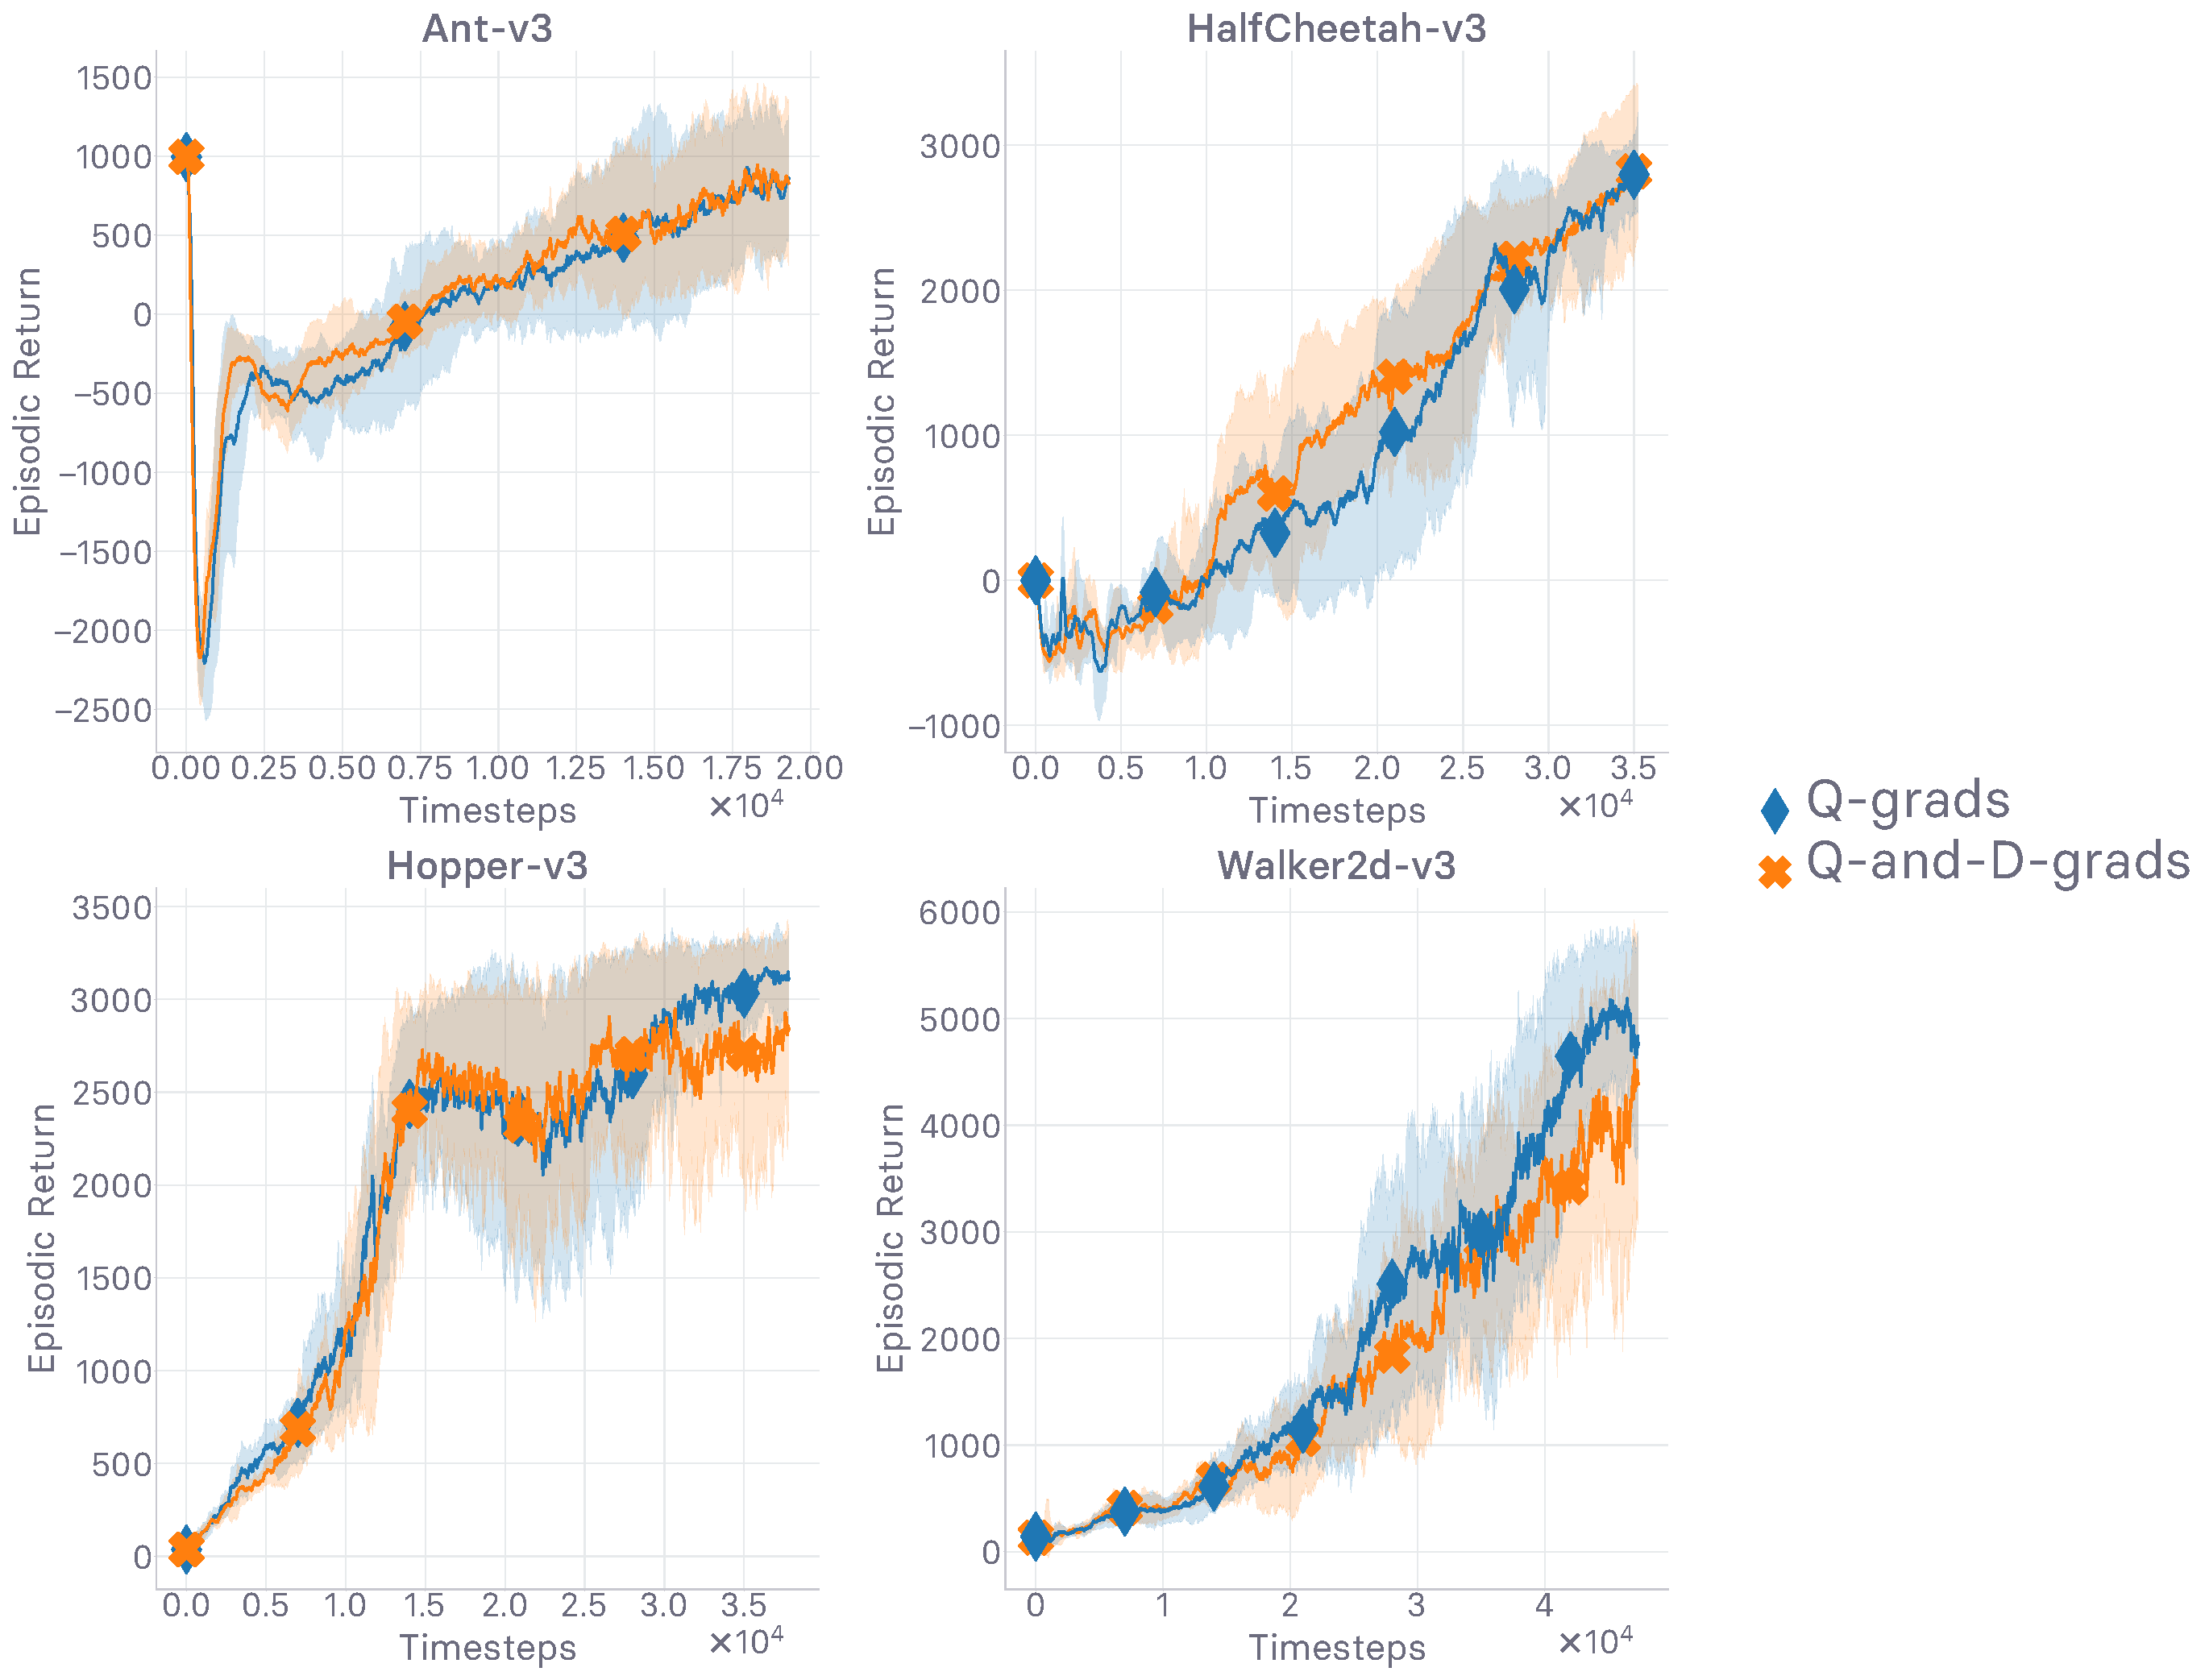
\includegraphics{Plots/fig12_ada_4envs/plots_eval_env_ret_plot.pdf}}
    \caption{Evolution of return values \textit{(higher is better)}}
  \end{subfigure}
  \begin{subfigure}[t]{0.49\textwidth}
    \center\scalebox{0.15}[0.15]{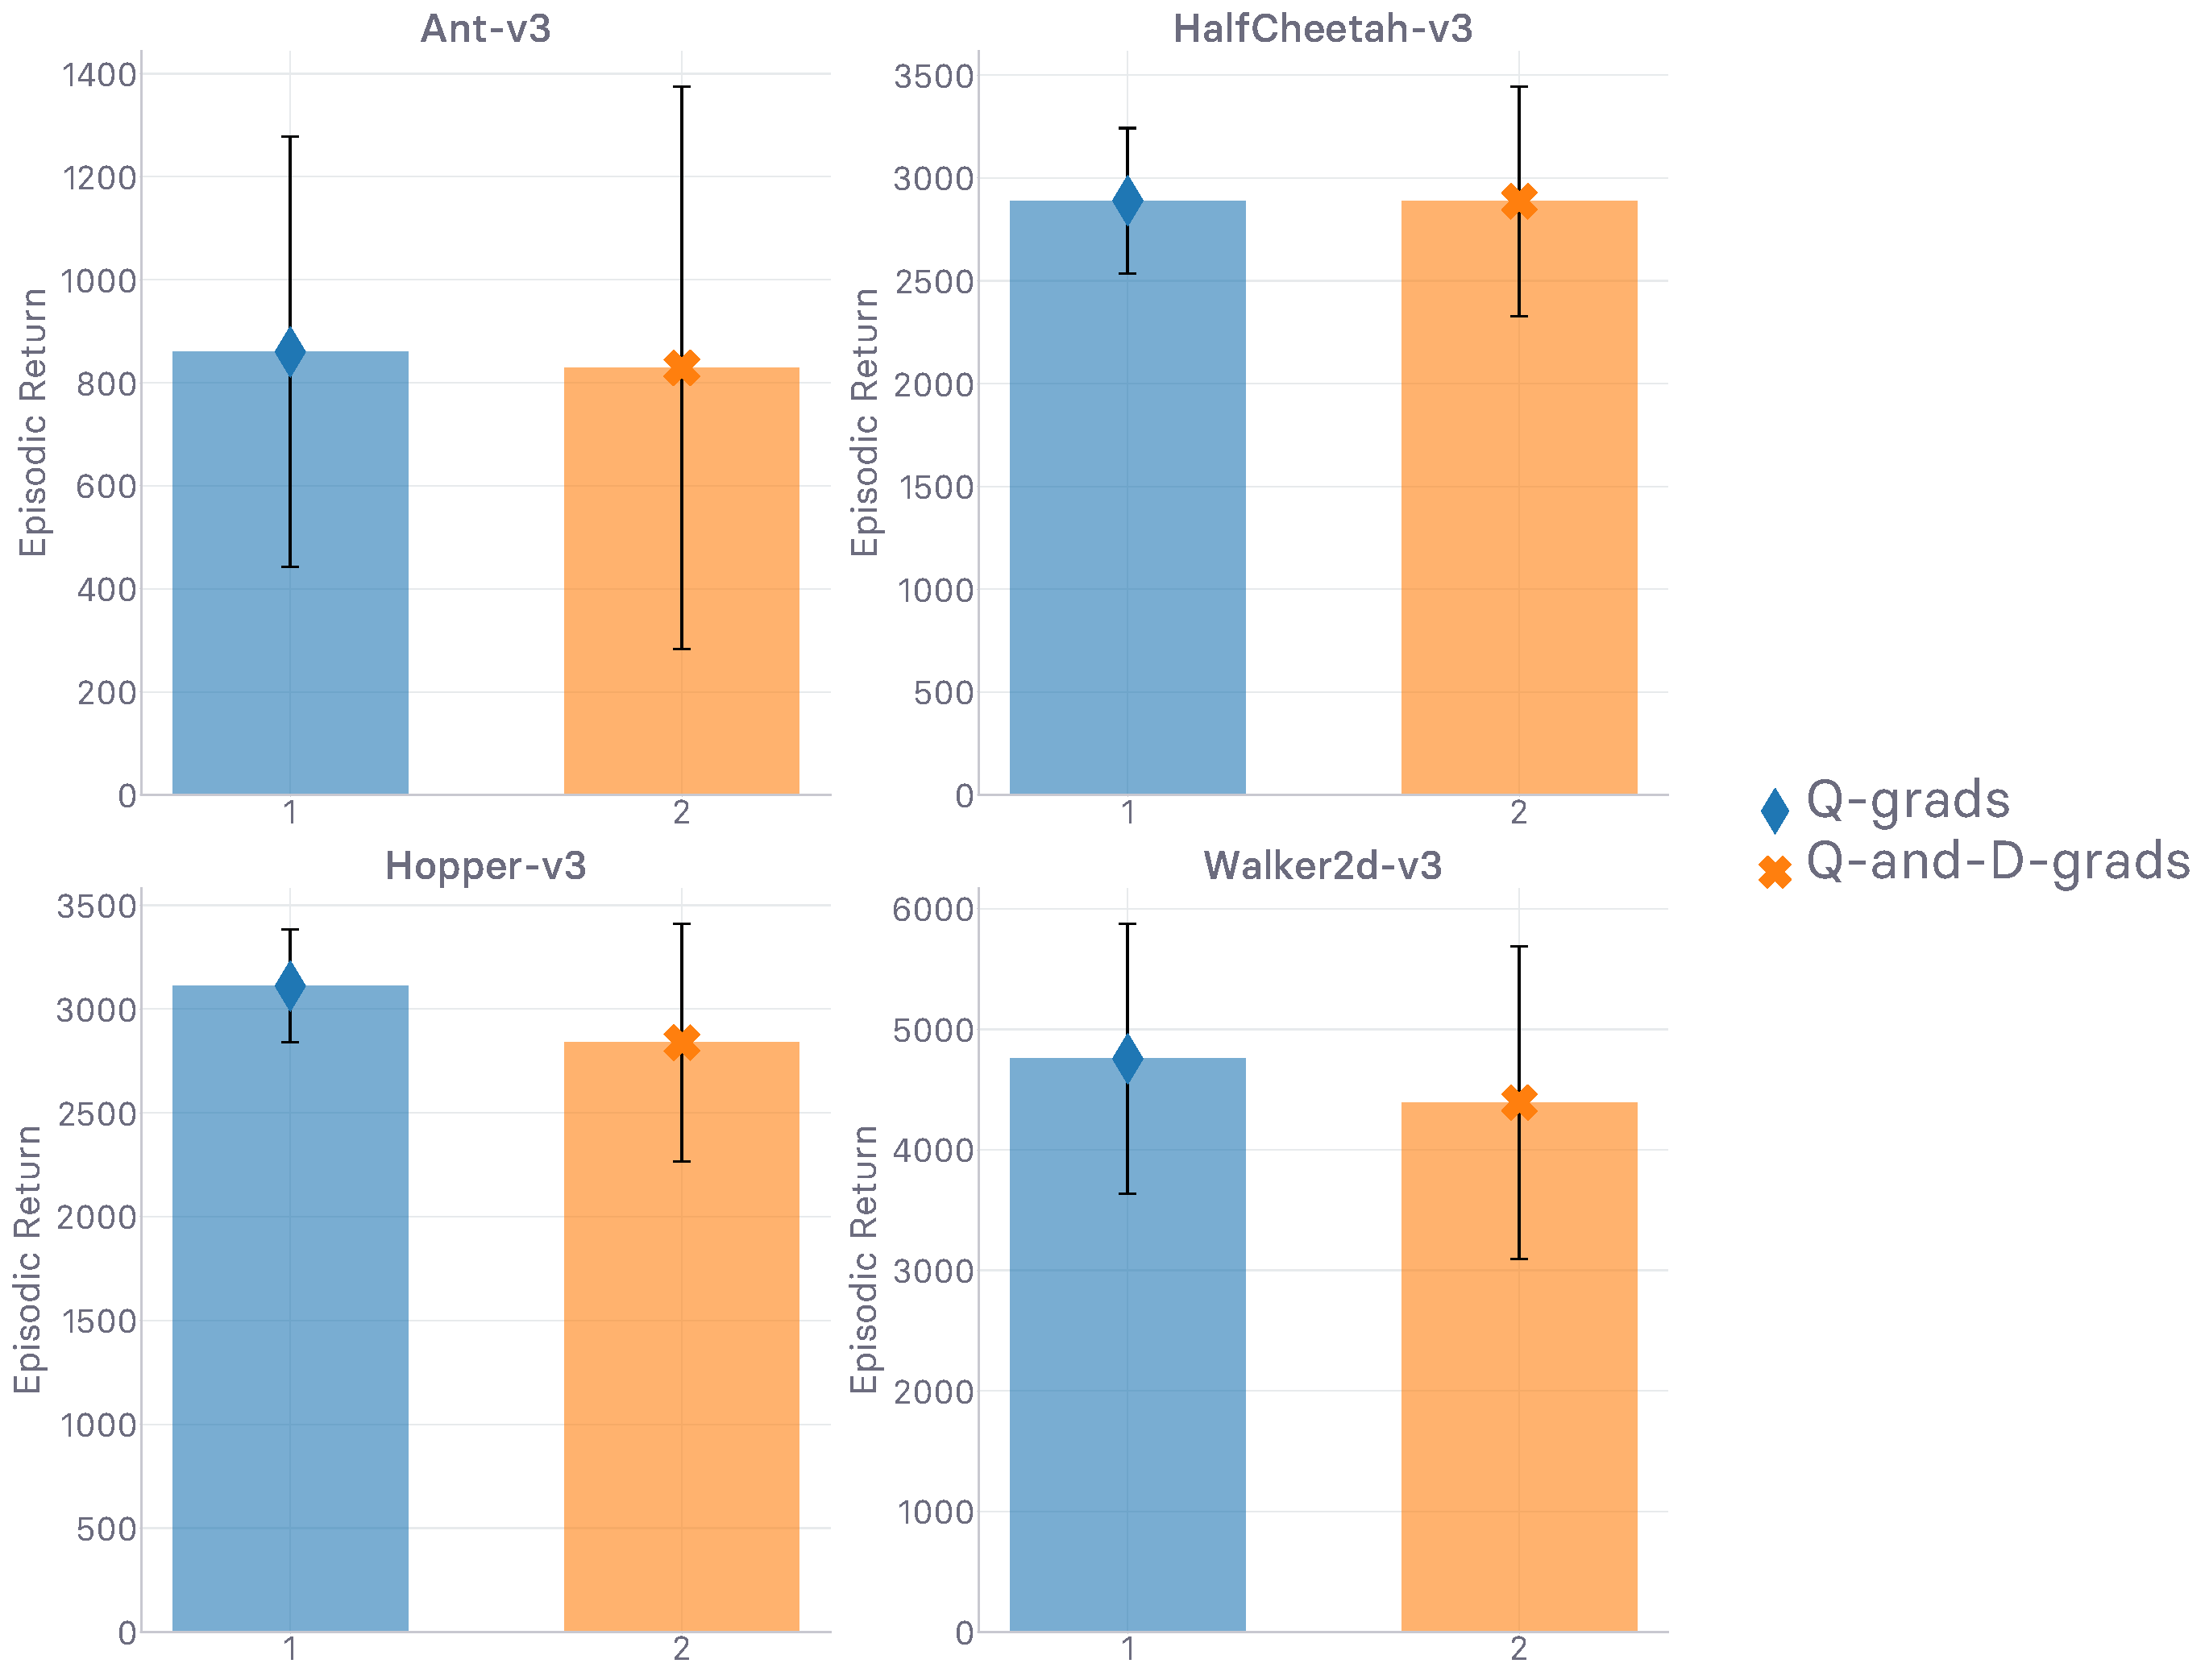
\includegraphics{Plots/fig12_ada_4envs/plots_eval_env_ret_barplot.pdf}}
    \caption{Final return values at timeout \textit{(higher is better)}}
  \end{subfigure}
  \caption{
  Comparison of the gradient used to update the policy in this work,
  involving the gradient of the state-action value,
  against an adaptive hybrid method involving \emph{also}
  the gradient of the discriminator, and combining both gradients
  based on their cosine similarity.
  Runtime is 12 hours.}
  \label{cosimplots}
\end{figure}

\section{Clipped Double-Q Learning and Target Policy Smoothing}
\label{ablationtd3}

\begin{figure}[H]
  \center
  \begin{subfigure}[t]{0.99\textwidth}
    \center\scalebox{0.18}[0.18]{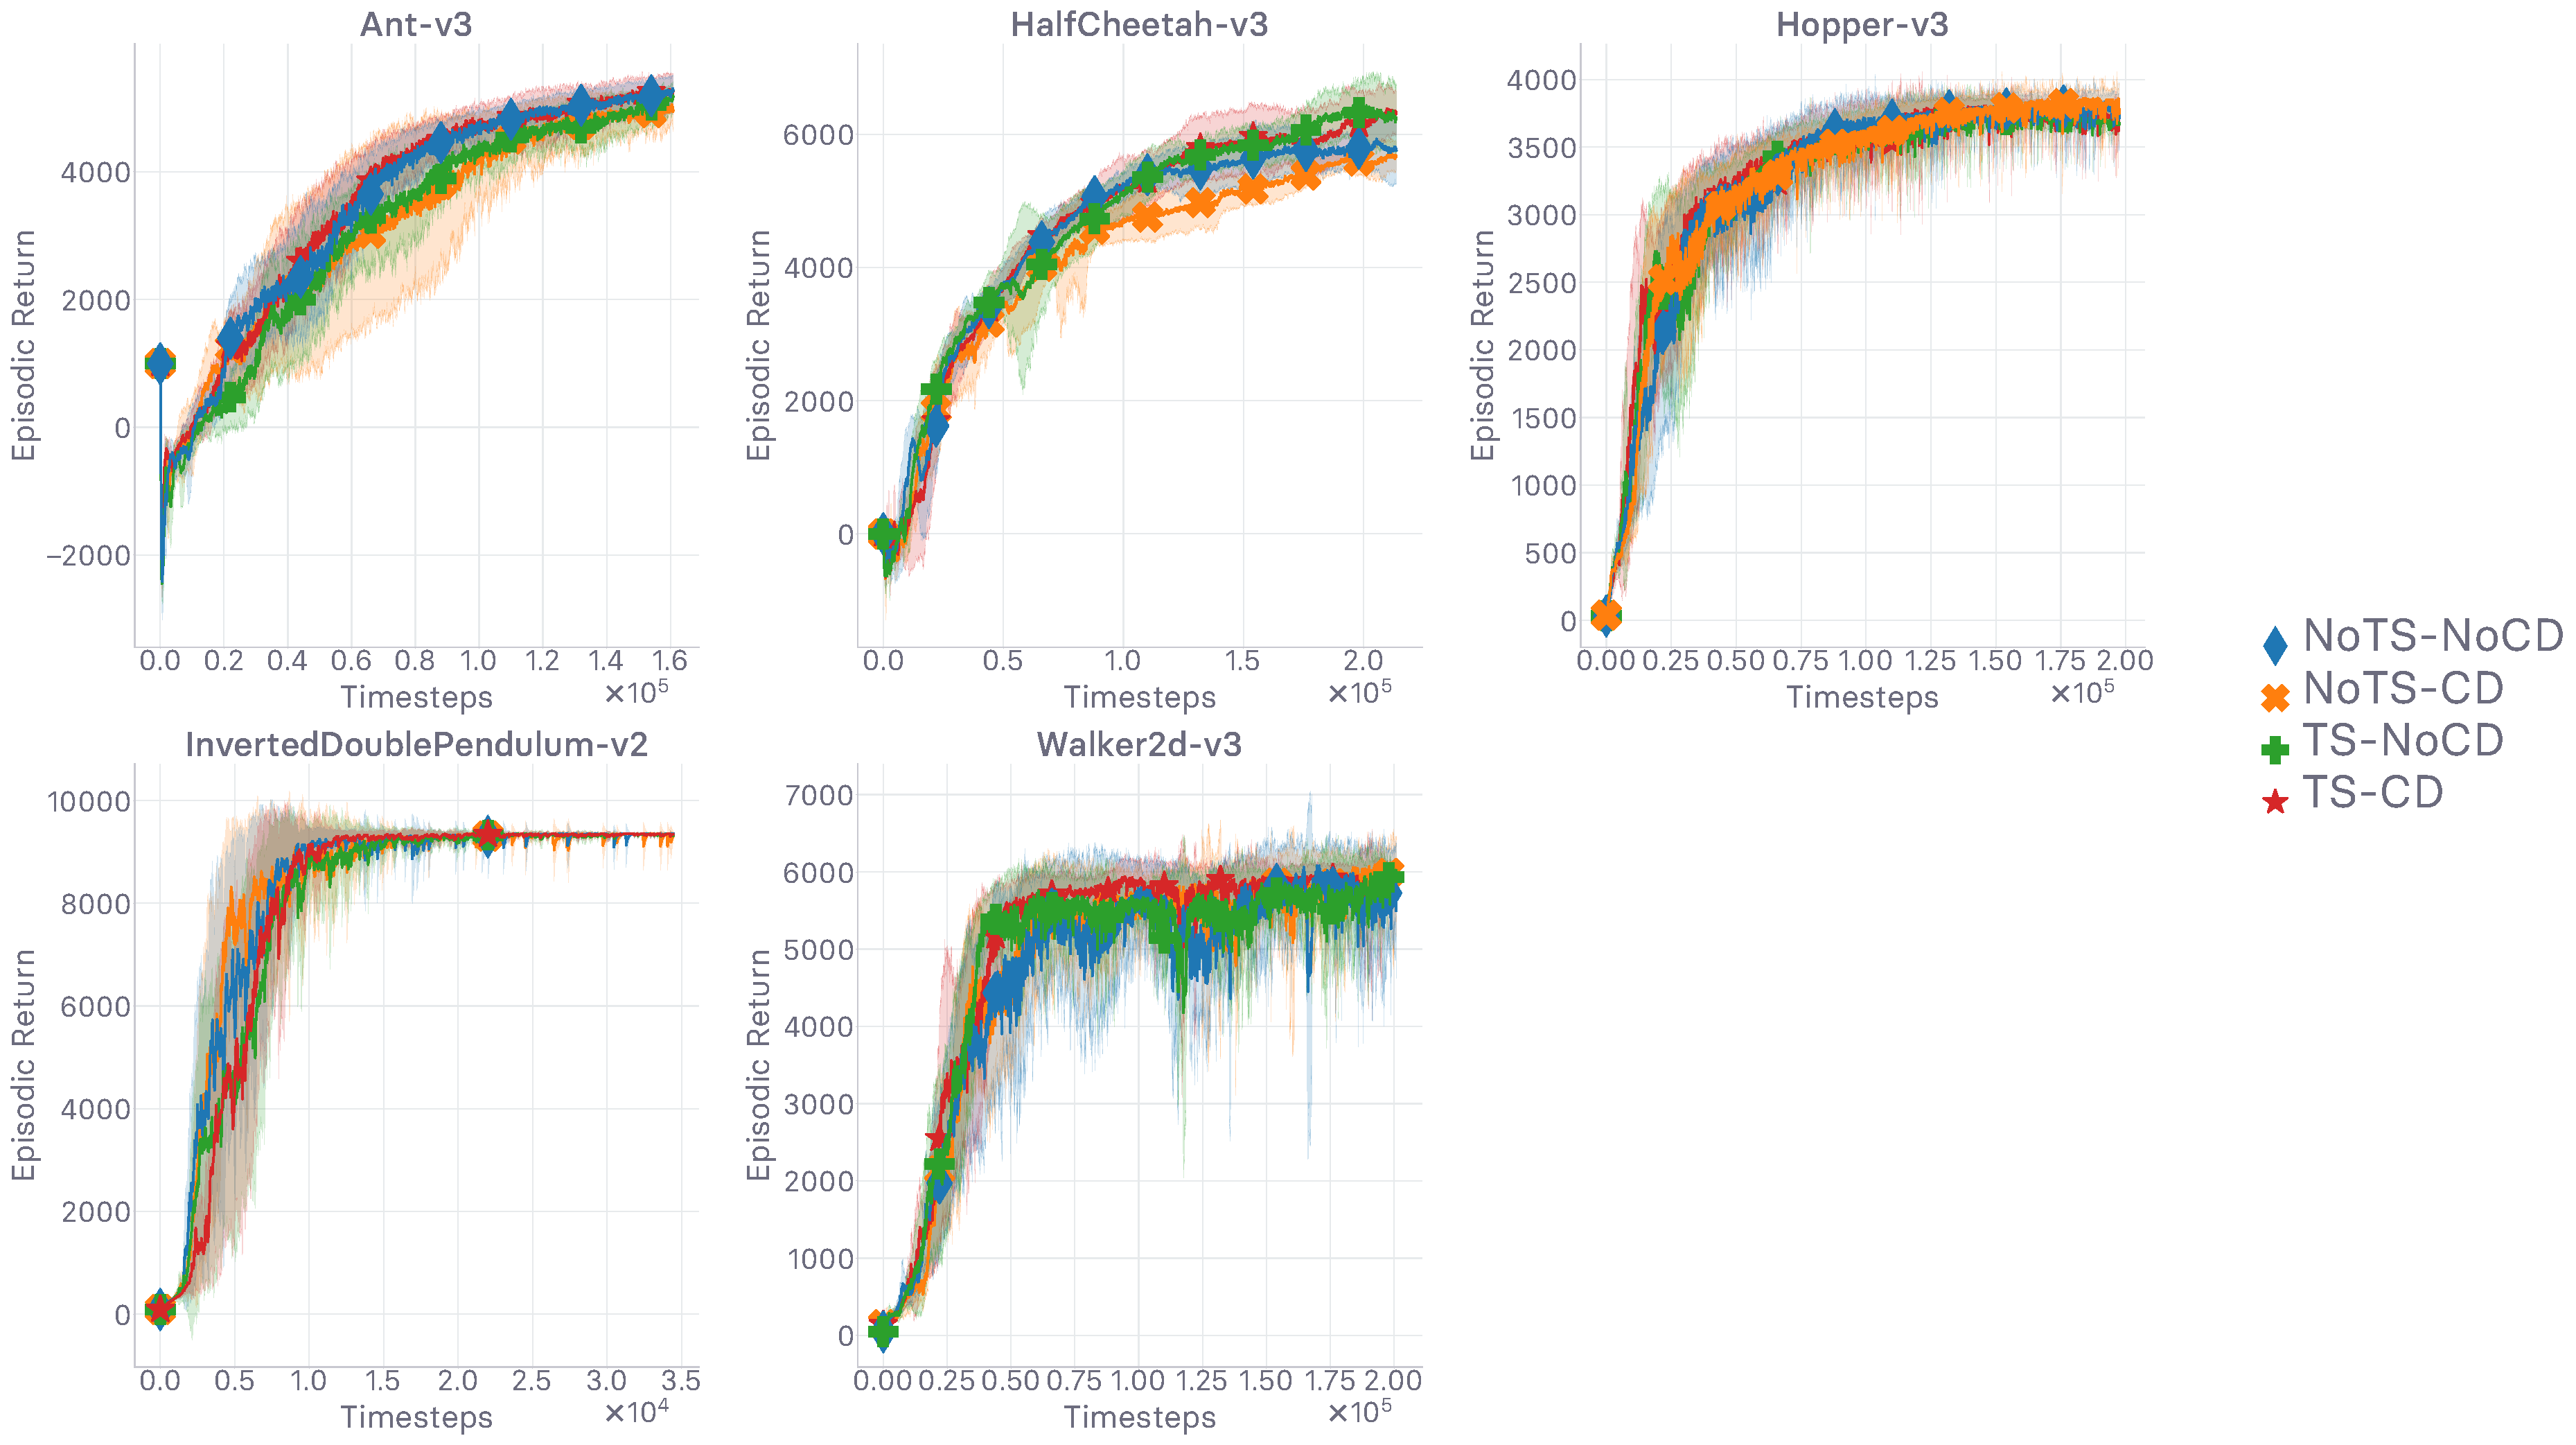
\includegraphics{Plots/fig13_td3_tricks_5envs/plots_eval_env_ret_plot.pdf}}
    \caption{Evolution of return values \textit{(higher is better)}}
  \end{subfigure}
  \begin{subfigure}[t]{0.99\textwidth}
    \center\scalebox{0.18}[0.18]{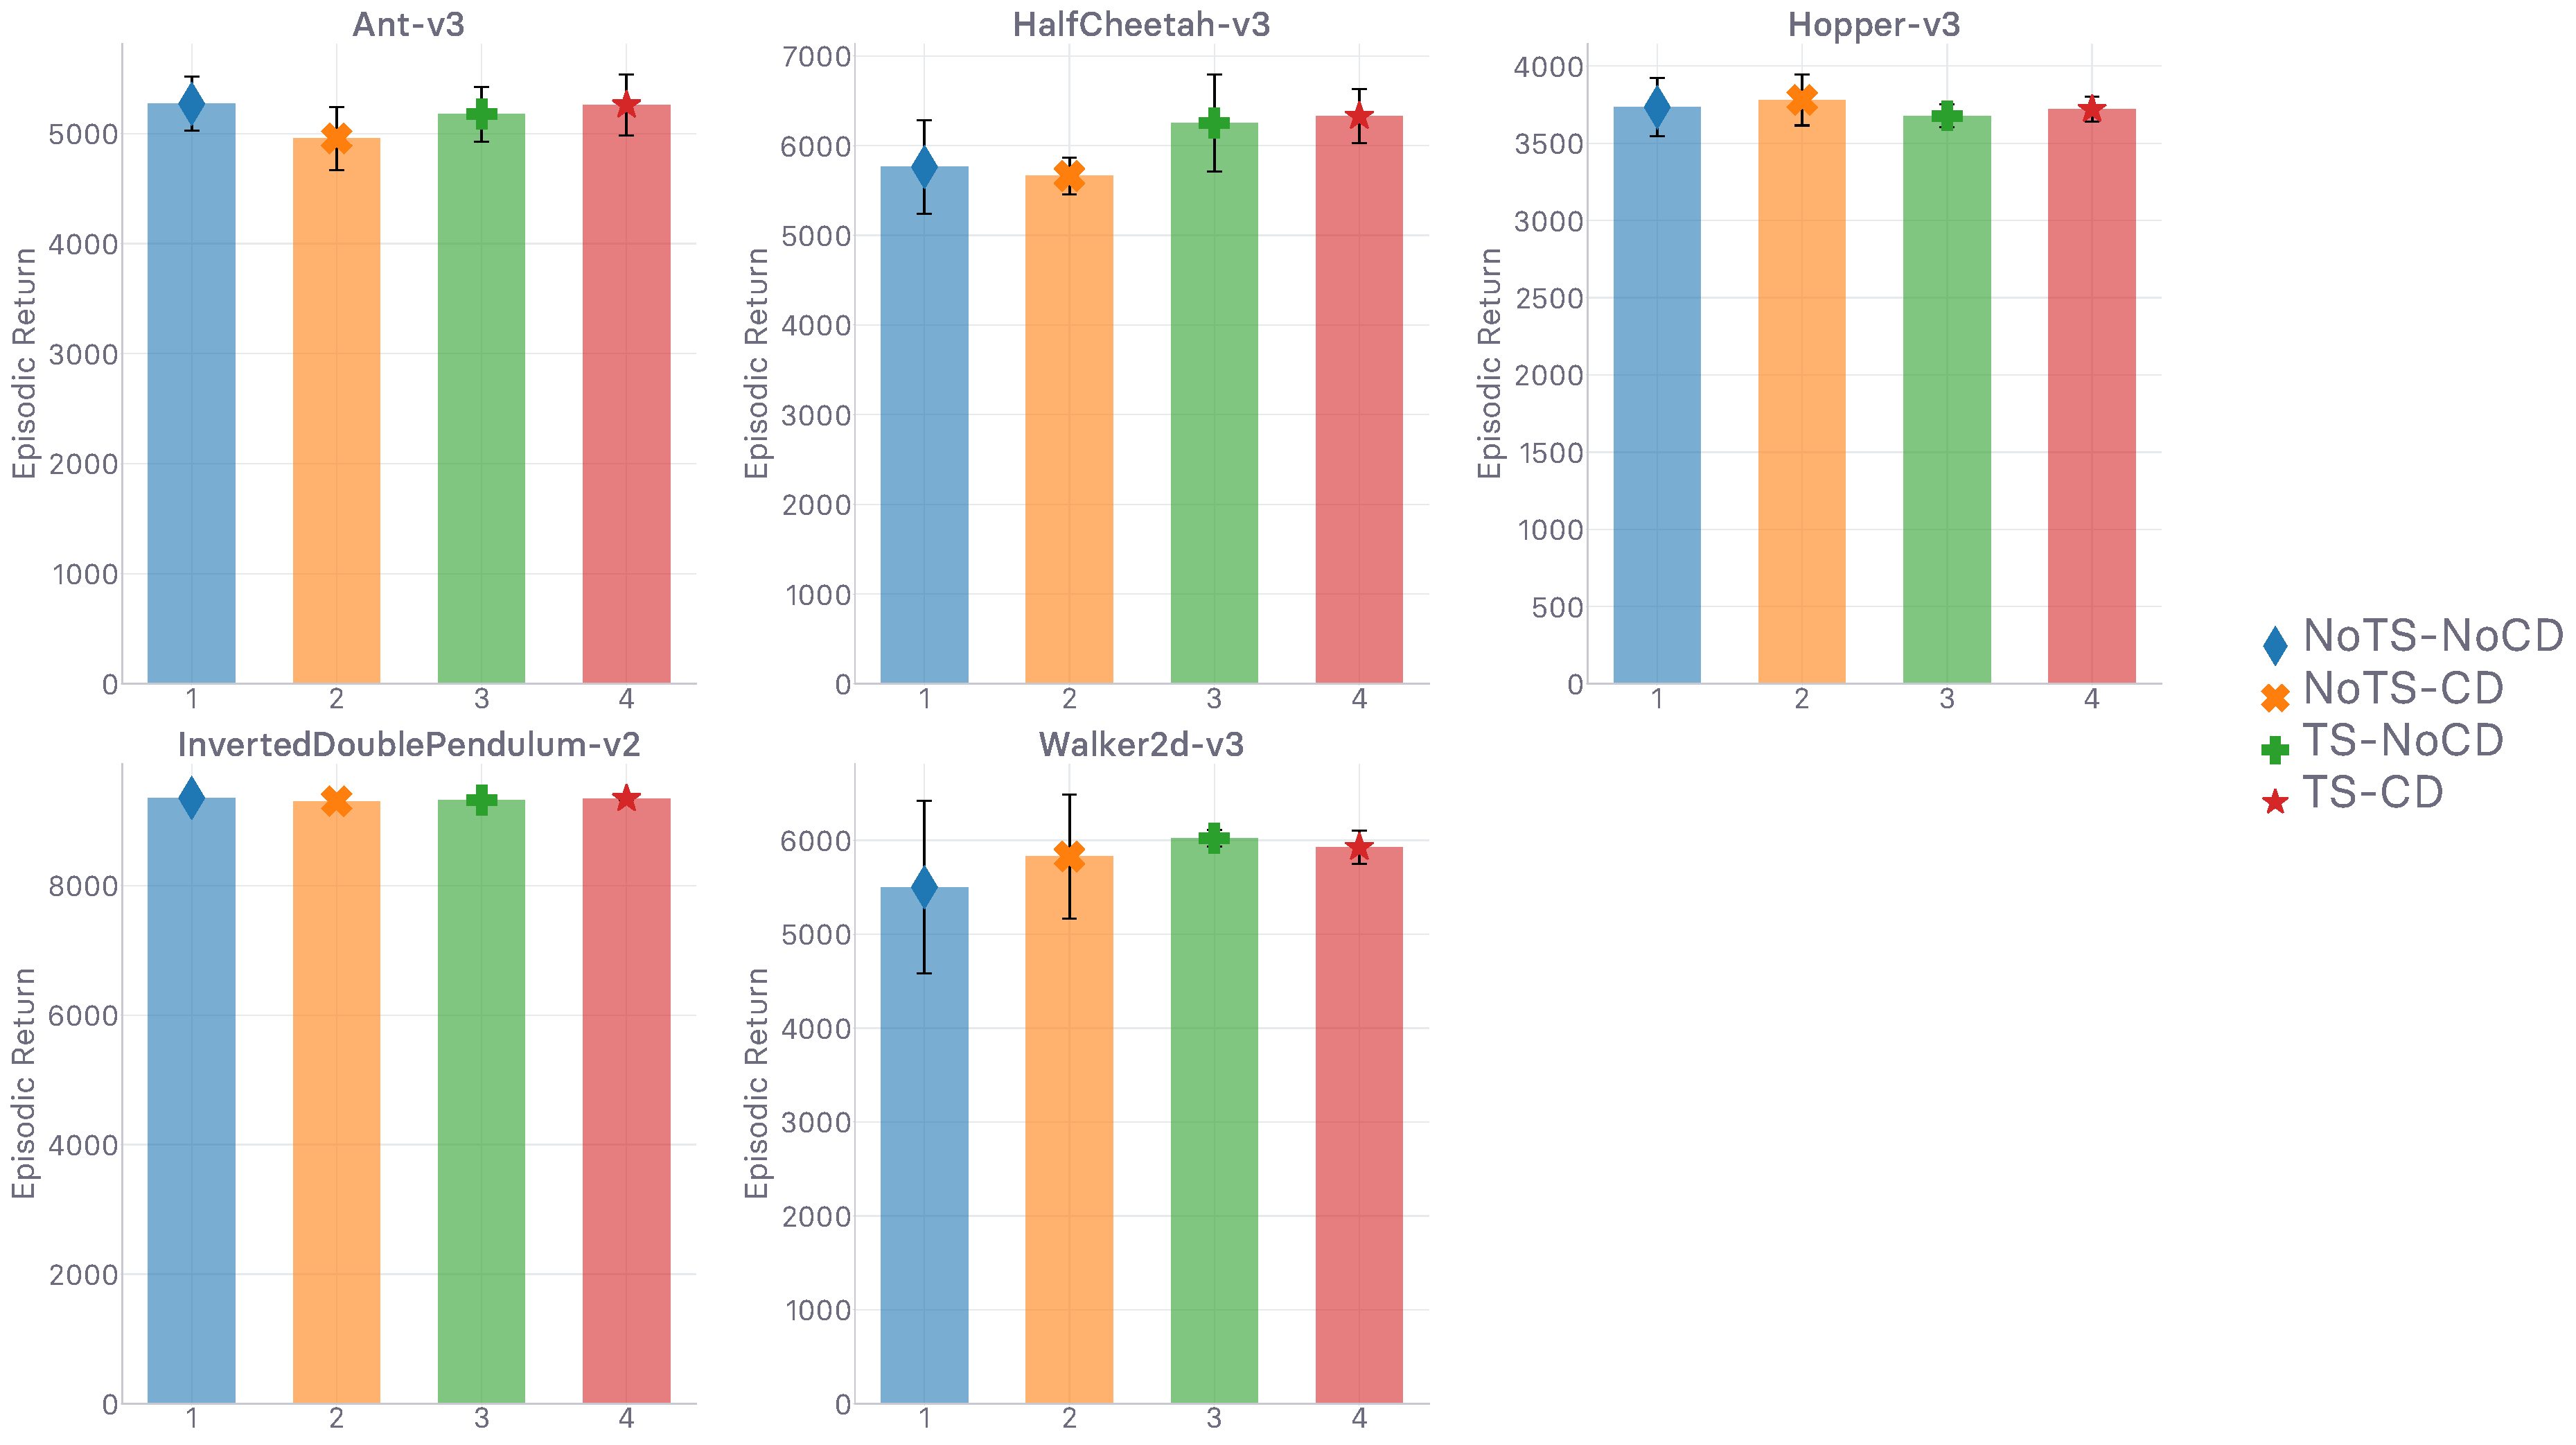
\includegraphics{Plots/fig13_td3_tricks_5envs/plots_eval_env_ret_barplot.pdf}}
    \caption{Final return values at timeout \textit{(higher is better)}}
  \end{subfigure}
  \caption{
  Ablation study on the use of the clipped double Q-Learning (CD)
  and target smoothing (TS) techniques,
  both from \cite{Fujimoto2018-pe},
  \emph{with} gradient penalty regularization \cite{Gulrajani2017-mr}.
  Runtime is 48 hours}
\end{figure}

\section{Gradient Penalty}

\subsection{One-sided Gradient Penalty}
\label{ablationonesided}

\begin{figure}[H]
  \center
  \begin{subfigure}[t]{0.99\textwidth}
    \center\scalebox{0.18}[0.18]{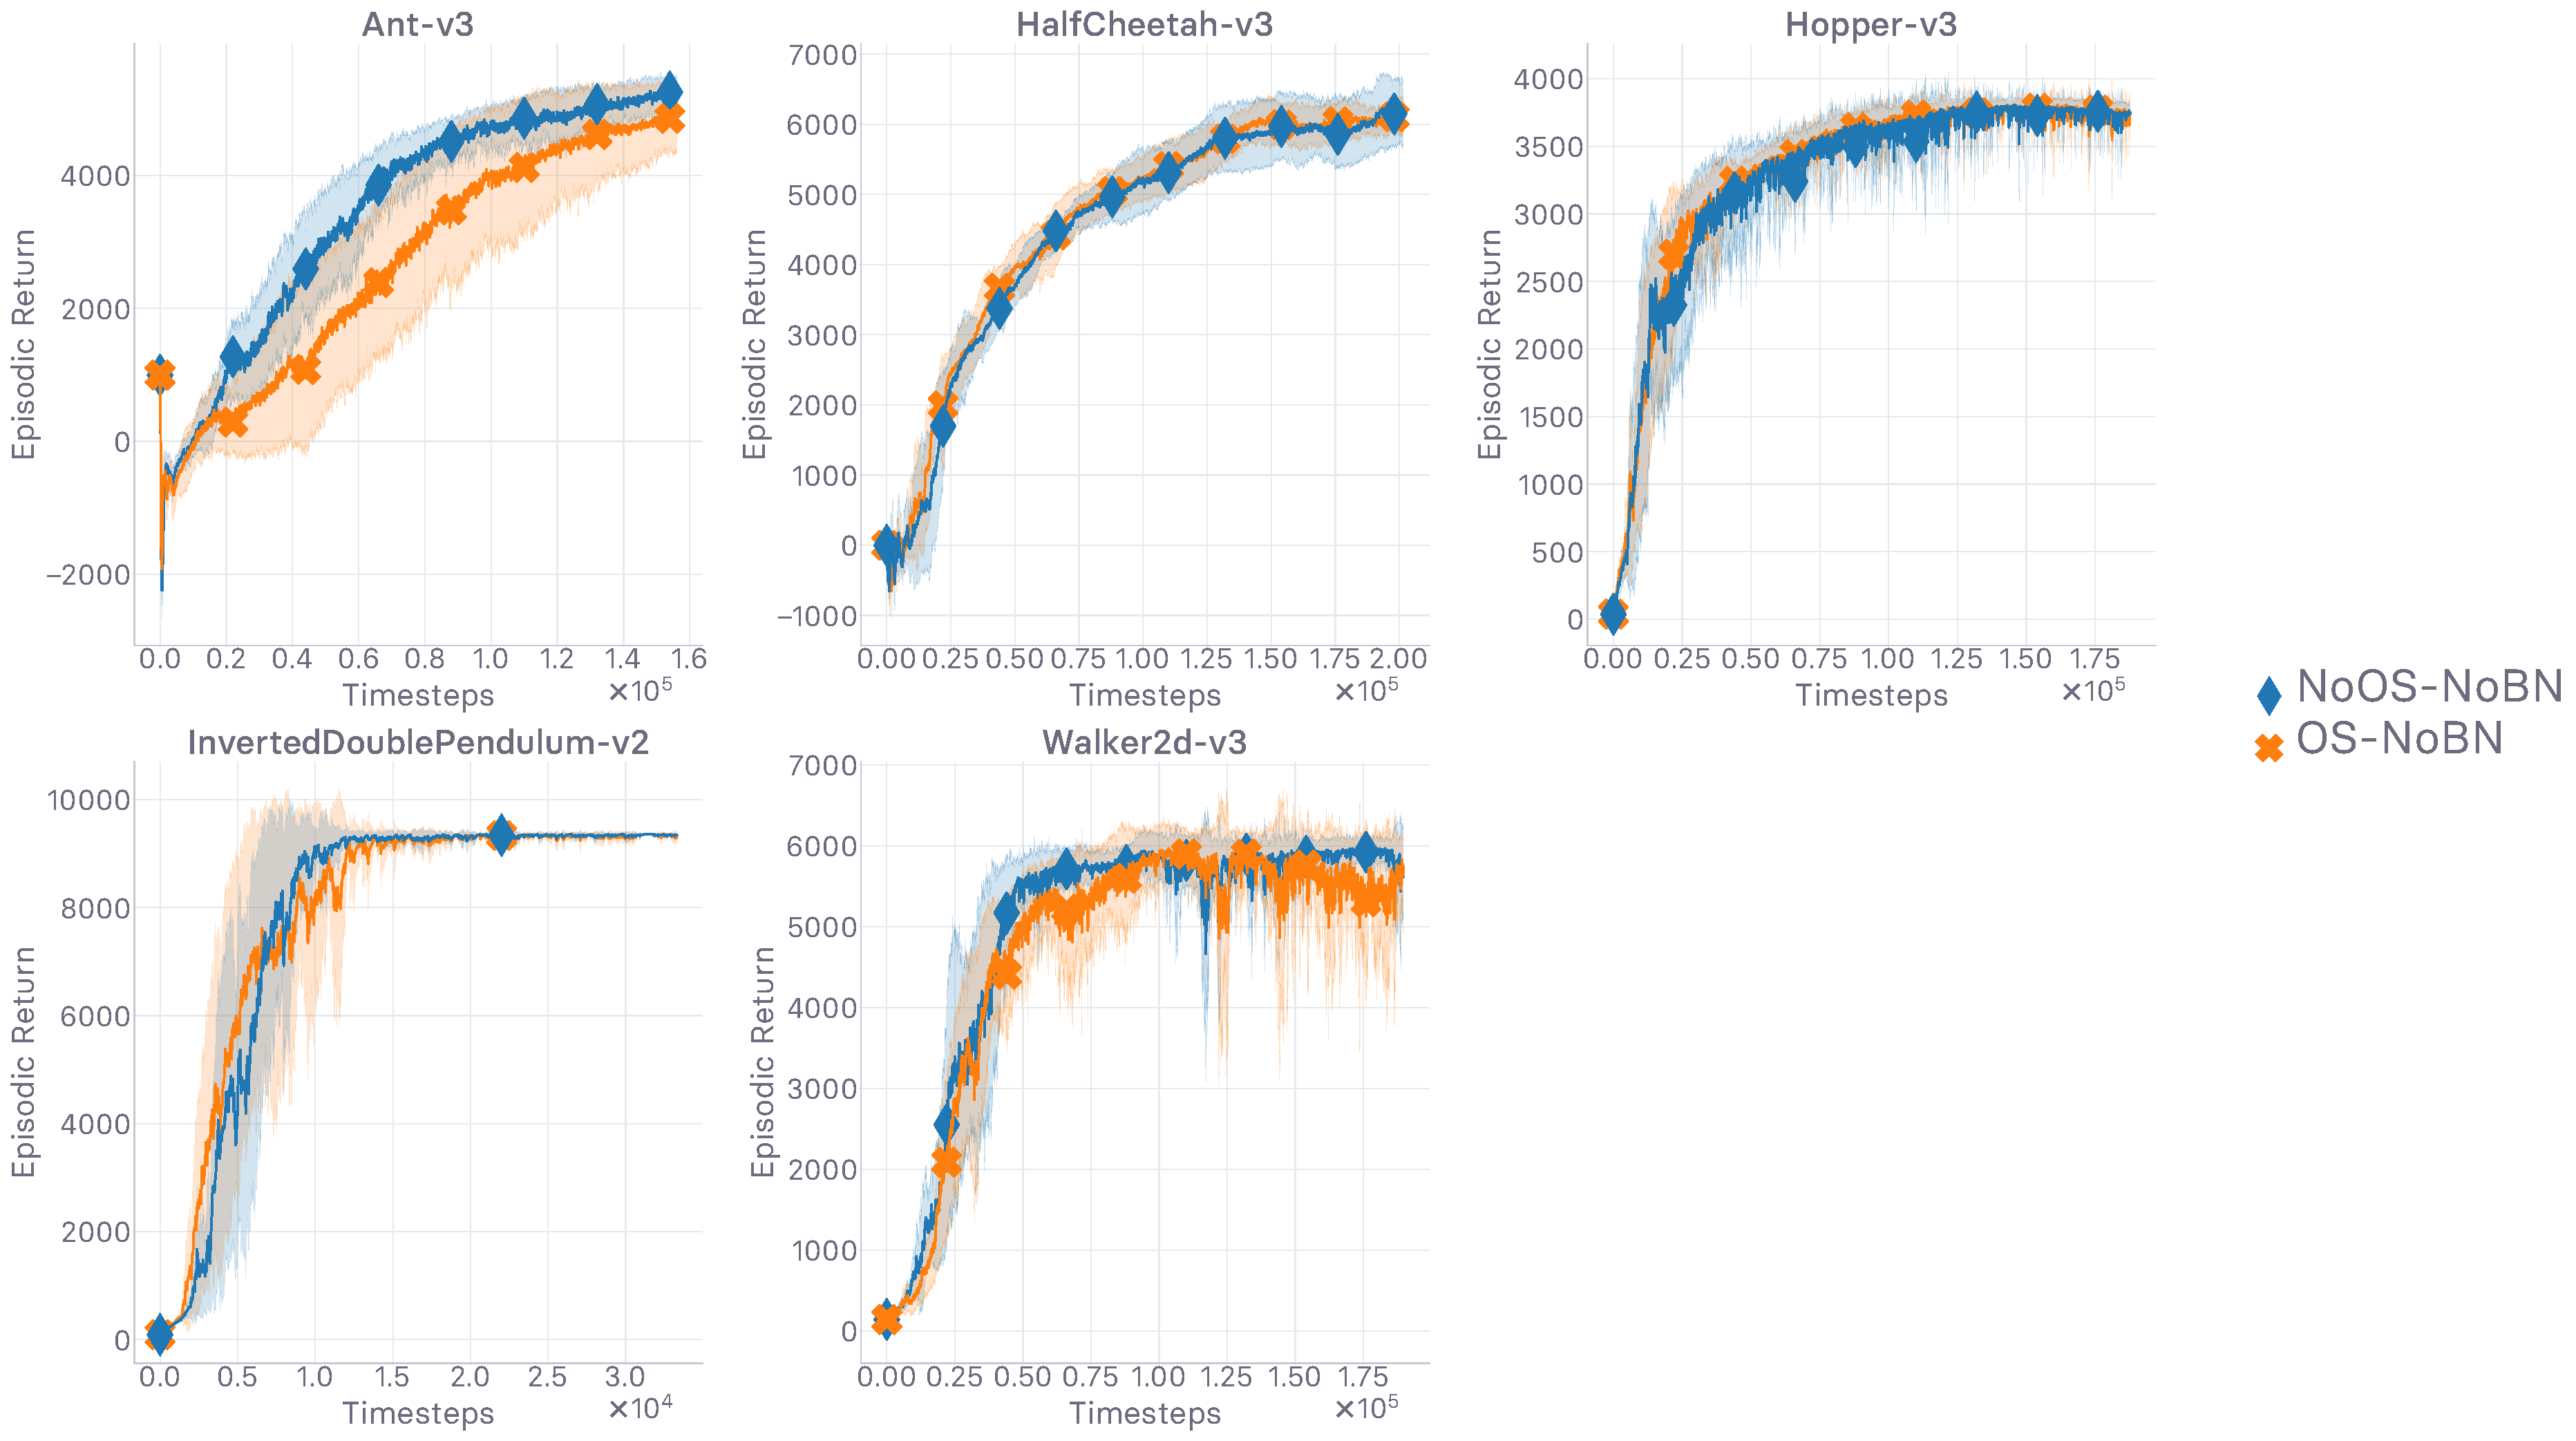
\includegraphics{Plots/fig14_os_ablation_5envs/plots_eval_env_ret_plot.pdf}}
    \caption{Evolution of return values \textit{(higher is better)}}
  \end{subfigure}
  \begin{subfigure}[t]{0.99\textwidth}
    \center\scalebox{0.18}[0.18]{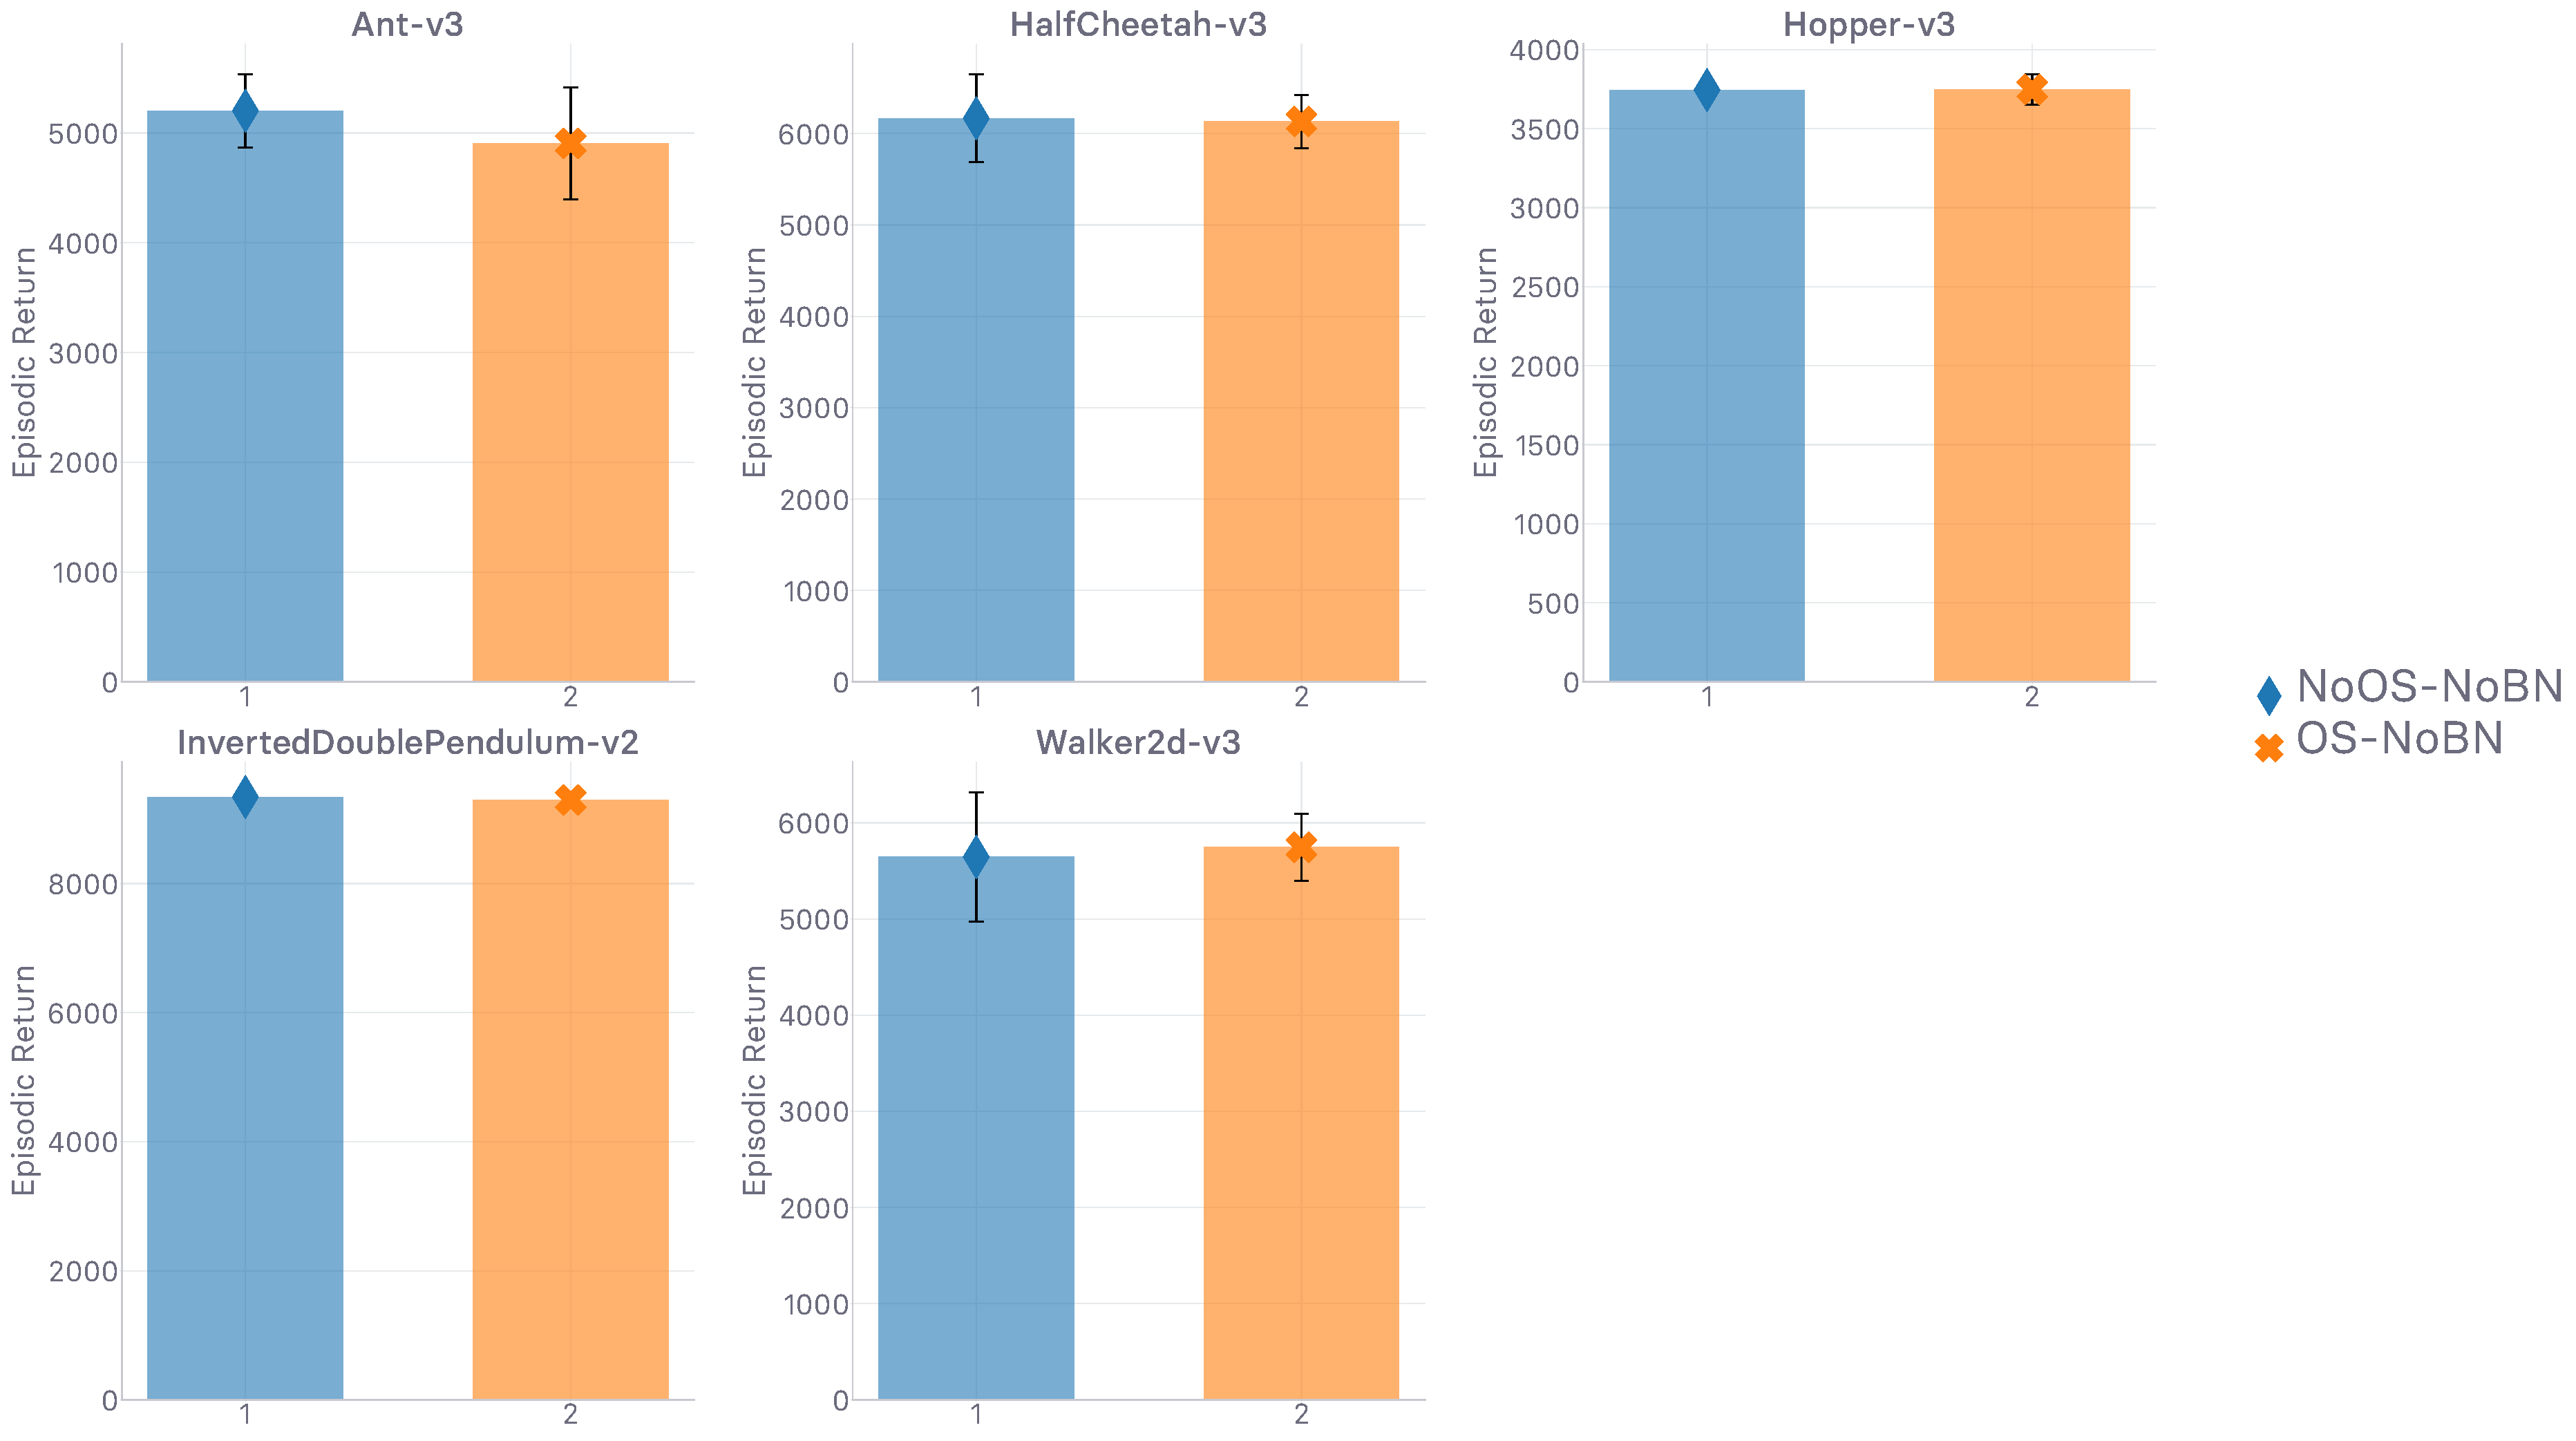
\includegraphics{Plots/fig14_os_ablation_5envs/plots_eval_env_ret_barplot.pdf}}
    \caption{Final return values at timeout \textit{(higher is better)}}
  \end{subfigure}
  \caption{
  Ablation study on the use of the one-sided (OS) penalty variant \cite{Gulrajani2017-mr}.
  Runtime is 48 hours}
\end{figure}

\subsection{Online Batch Normalization in Discriminator}
\label{ablationbn}

\begin{figure}[H]
  \center
  \begin{subfigure}[t]{0.99\textwidth}
    \center\scalebox{0.18}[0.18]{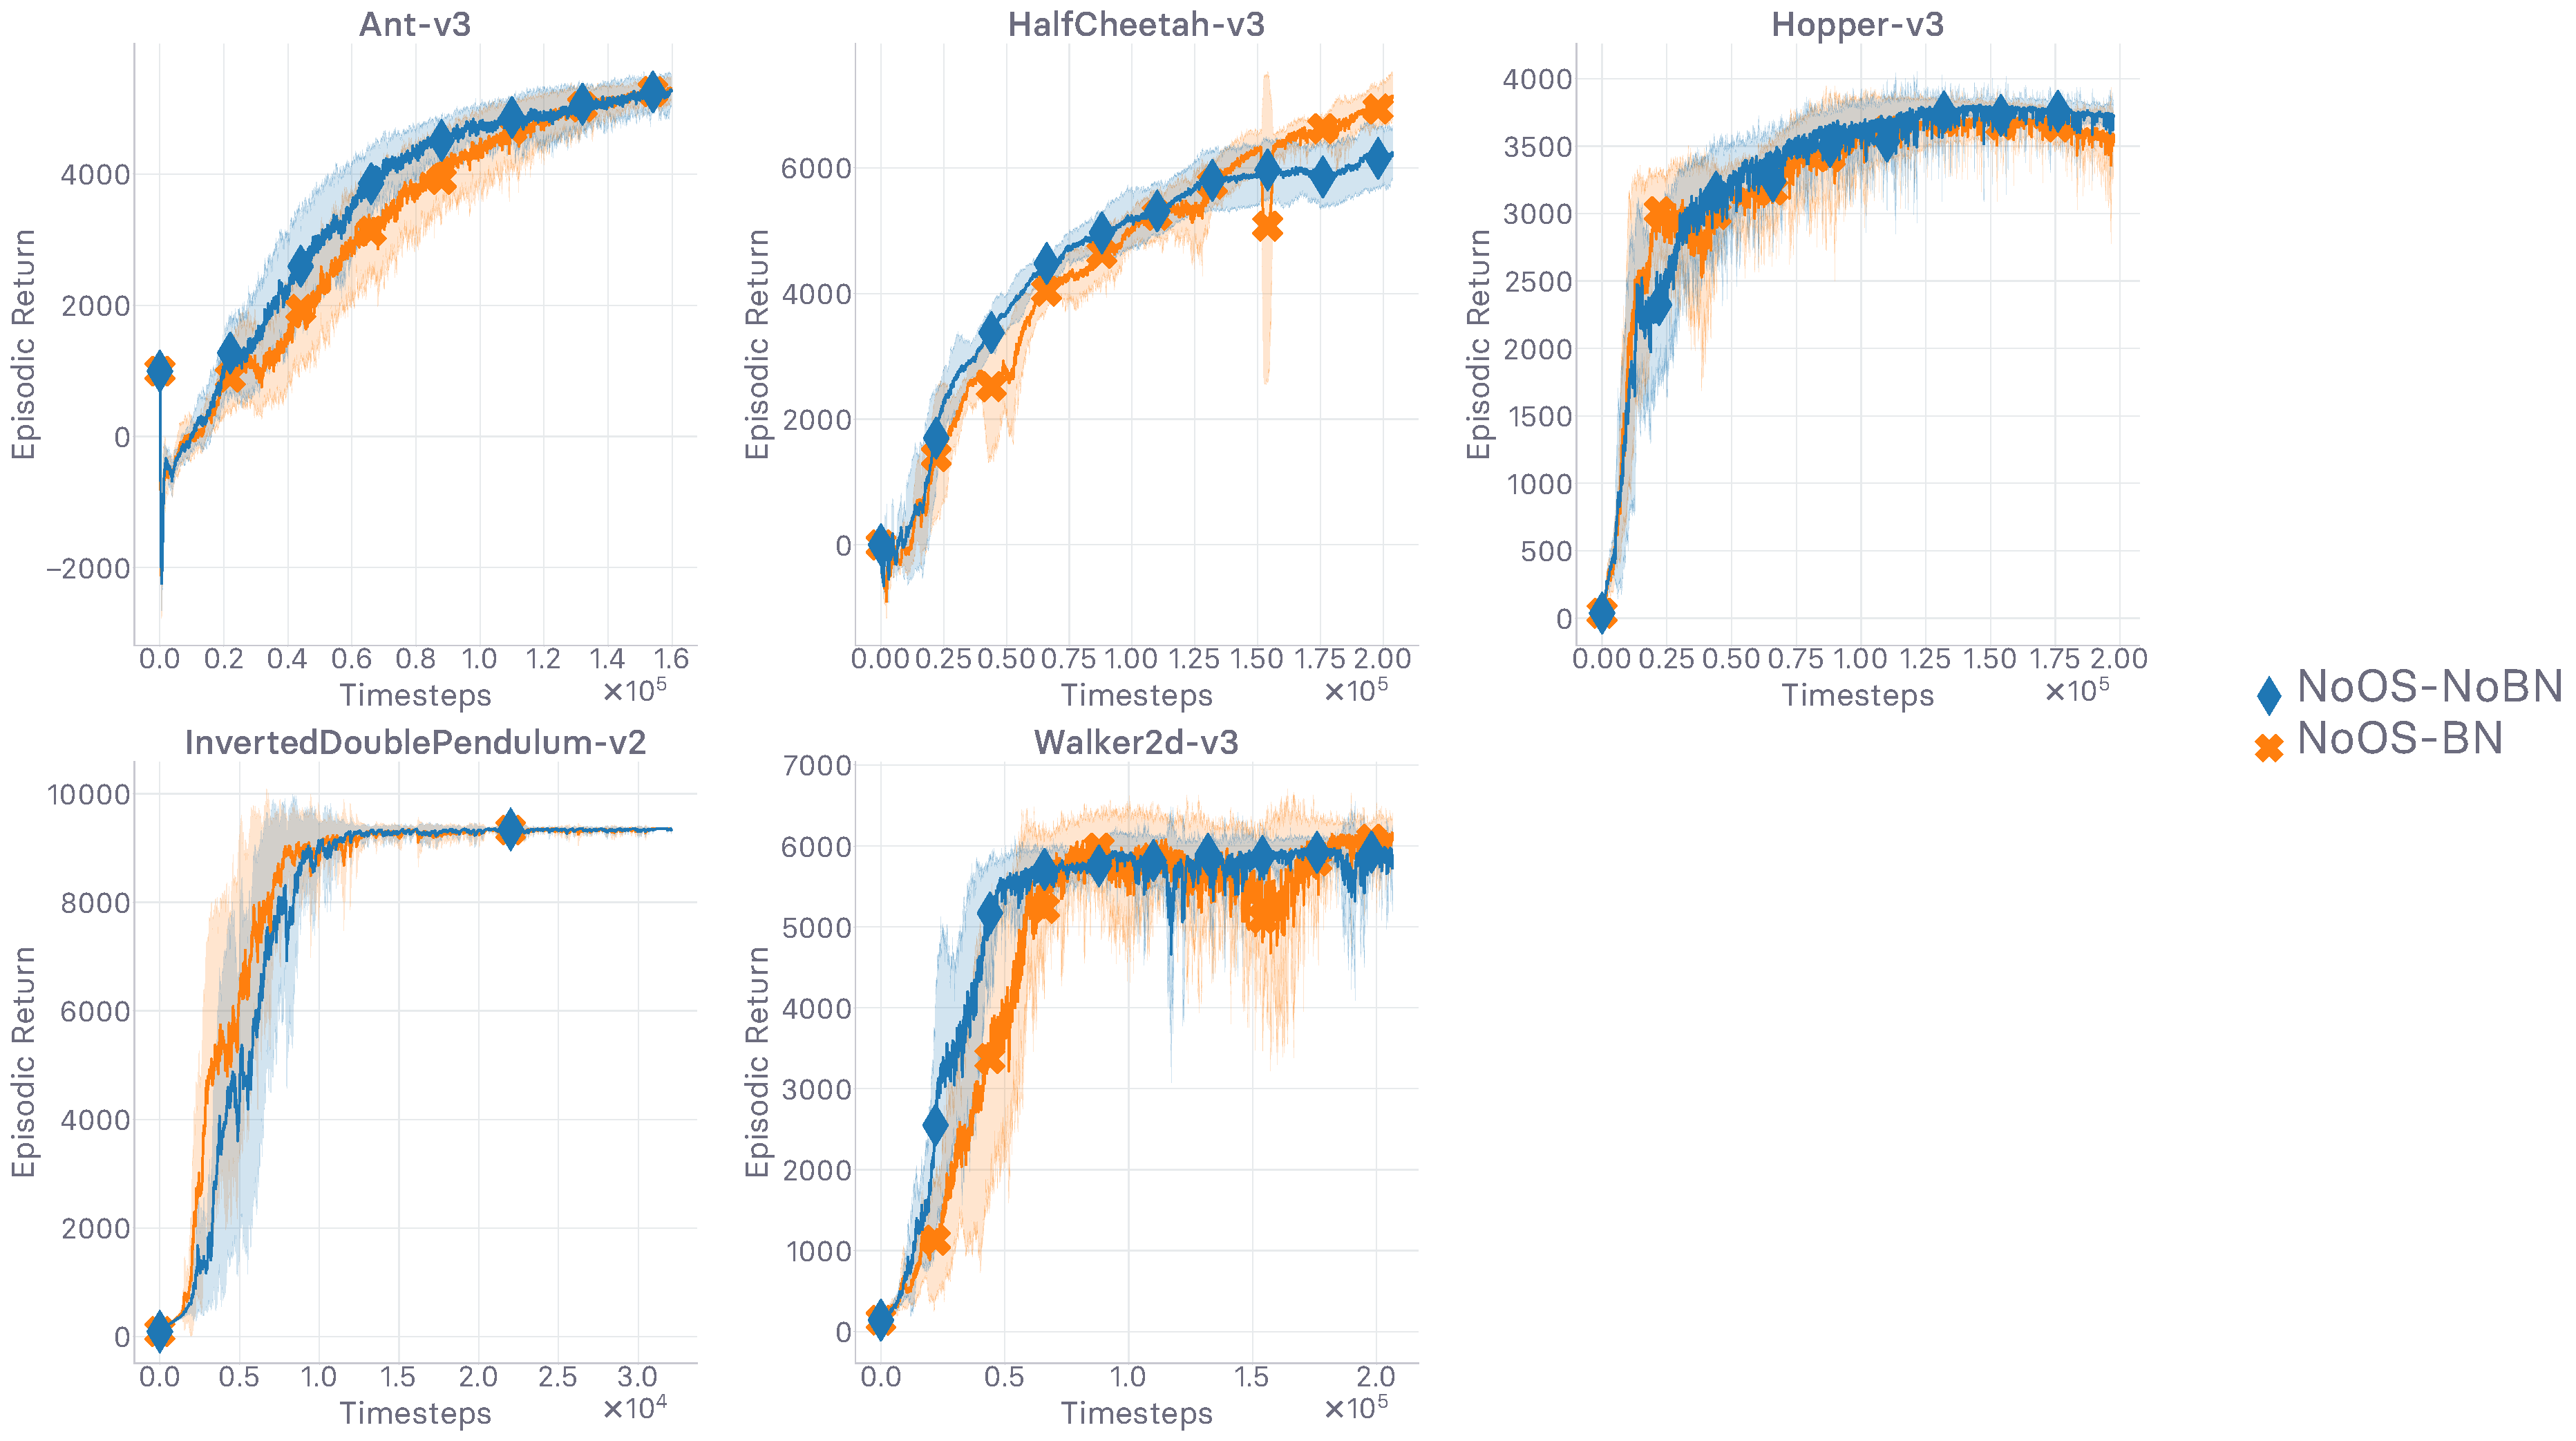
\includegraphics{Plots/fig15_bs_ablation_5envs/plots_eval_env_ret_plot.pdf}}
    \caption{Evolution of return values \textit{(higher is better)}}
  \end{subfigure}
  \begin{subfigure}[t]{0.99\textwidth}
    \center\scalebox{0.18}[0.18]{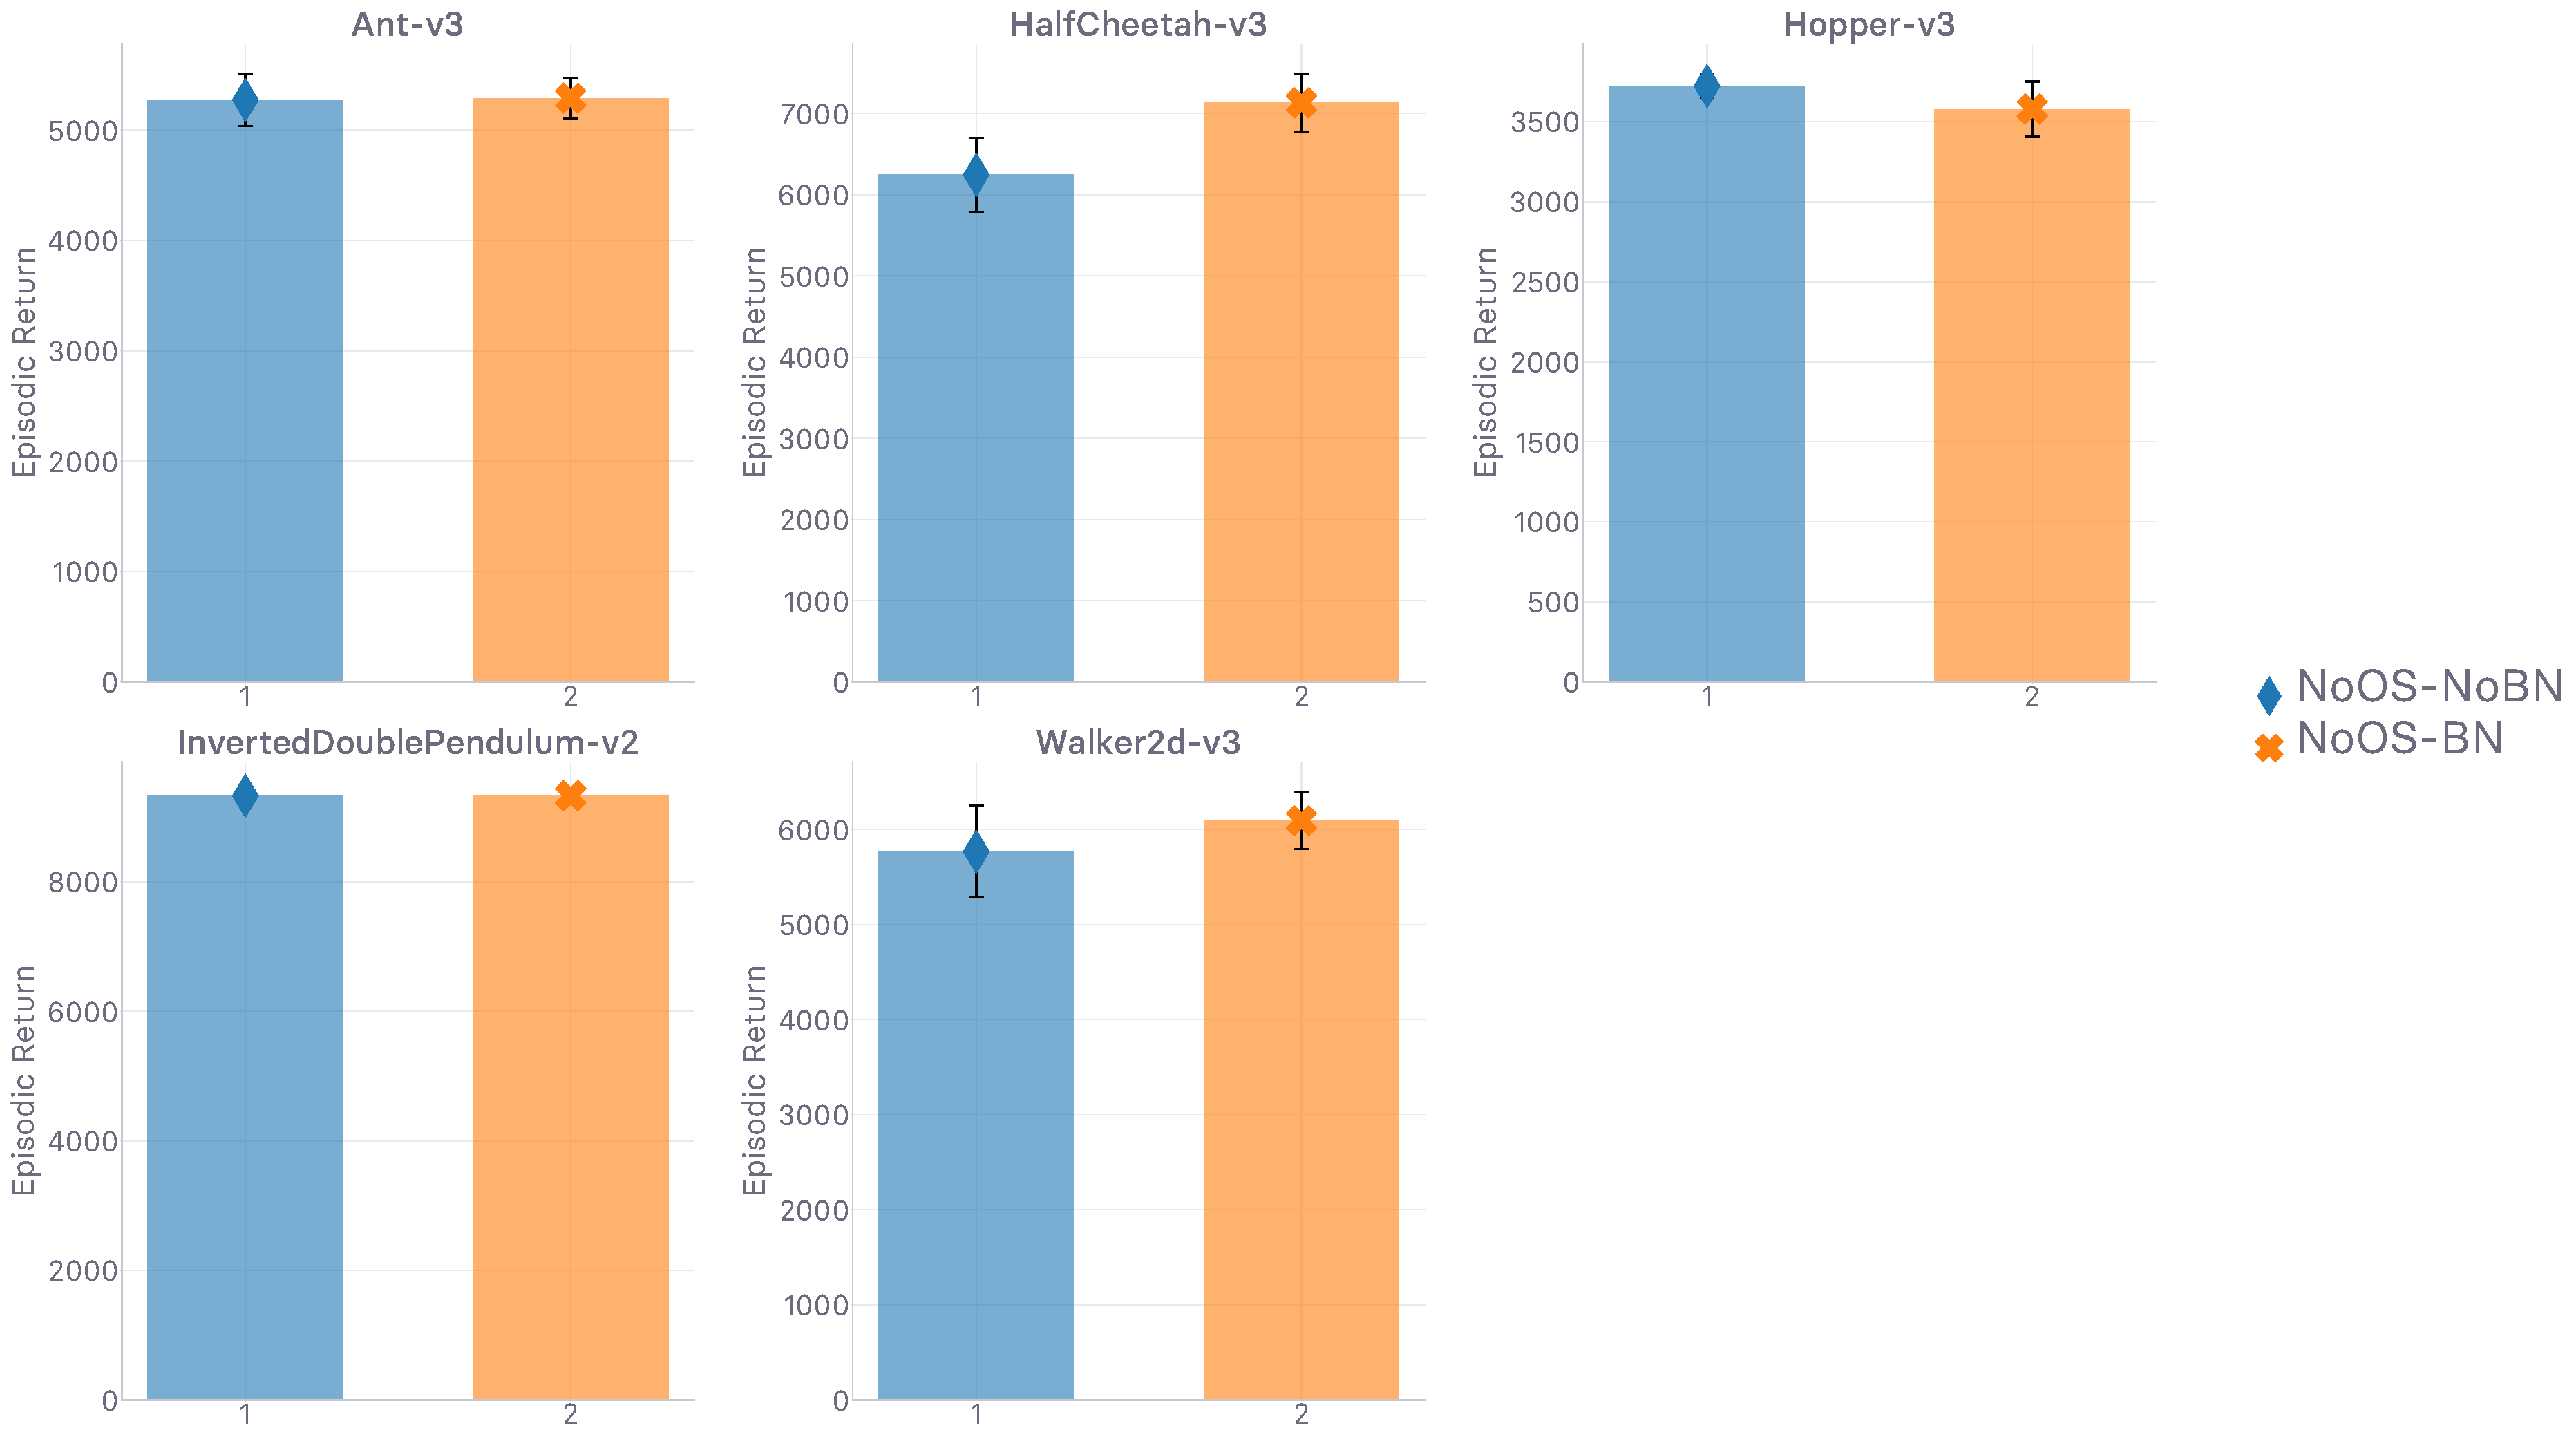
\includegraphics{Plots/fig15_bs_ablation_5envs/plots_eval_env_ret_barplot.pdf}}
    \caption{Final return values at timeout \textit{(higher is better)}}
  \end{subfigure}
  \caption{
  Ablation study on the use of online batch normalization (BN) in the
  discriminator for its impact on the gradient penalization \cite{Gulrajani2017-mr}.
  Runtime is 48 hours}
\end{figure}

\subsection{Target $k$ and Coefficient $\lambda$ Grid Search}
\label{gridklam}

\begin{figure}[H]
  \center
  \begin{subfigure}[t]{0.49\textwidth}
    \center\scalebox{0.15}[0.15]{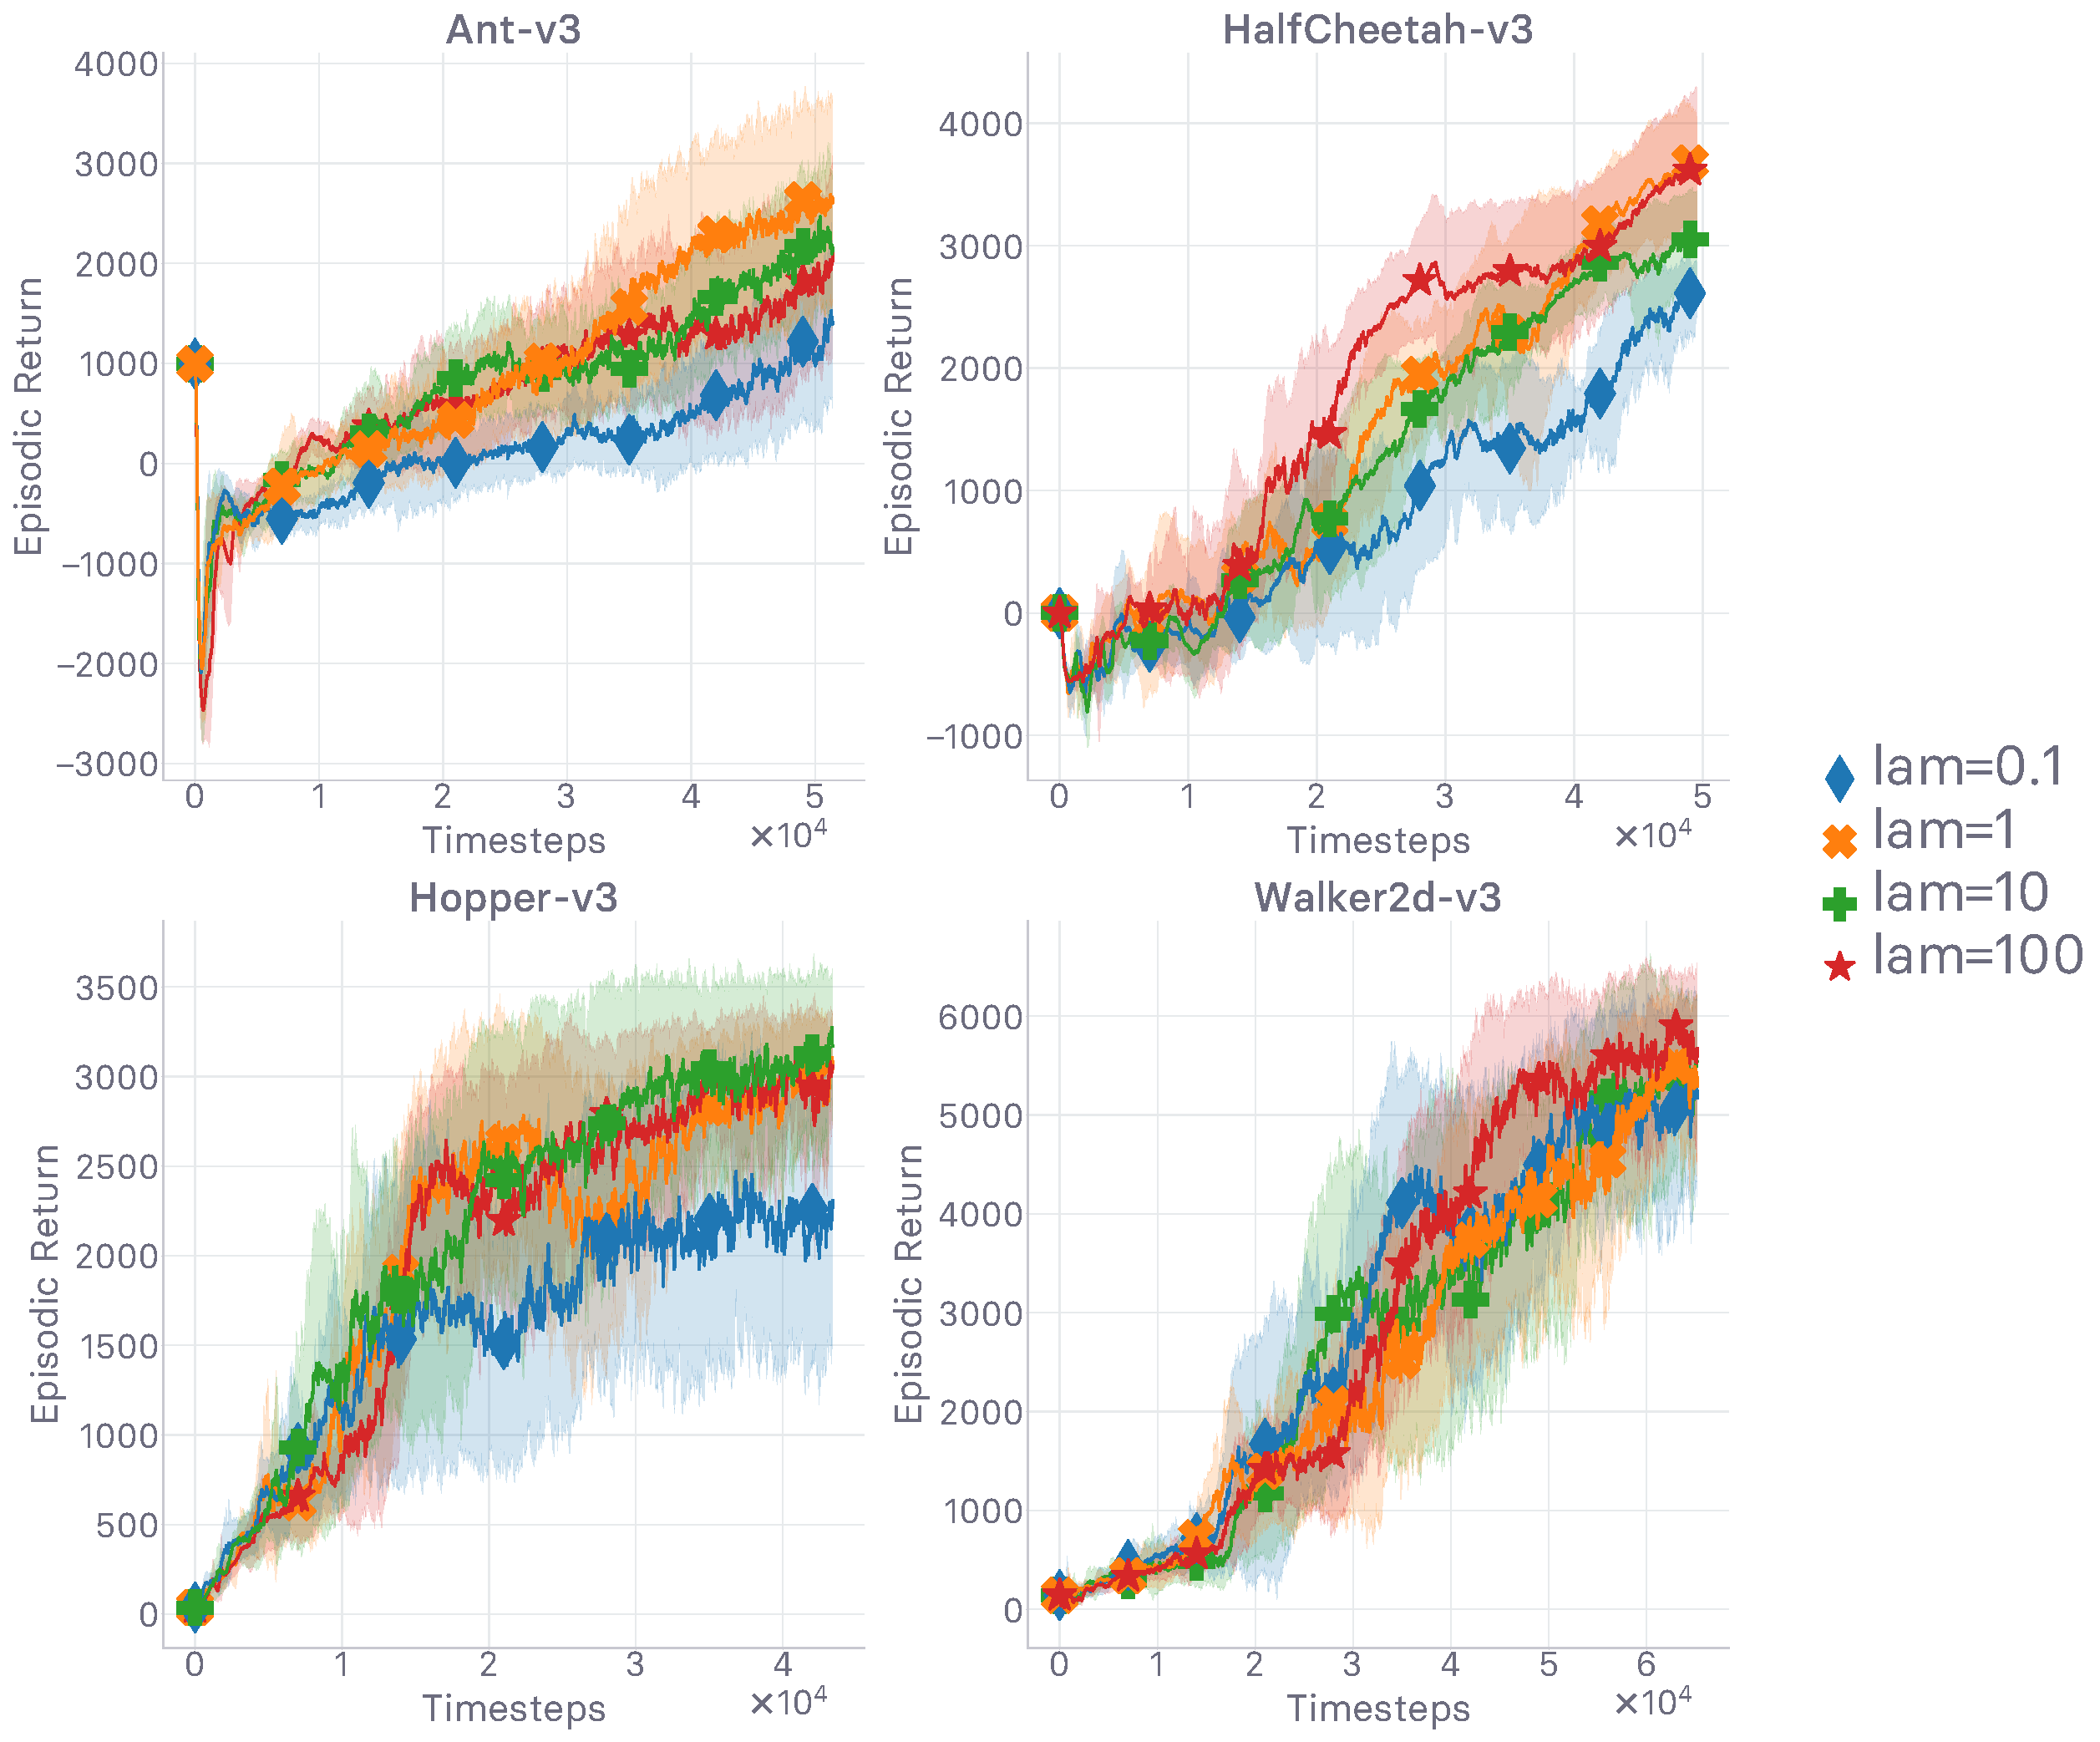
\includegraphics{Plots/fig16_k1_lam_gs_4envs/plots_eval_env_ret_plot.pdf}}
    \caption{Evolution of return values \textit{(higher is better)}}
  \end{subfigure}
  \begin{subfigure}[t]{0.49\textwidth}
    \center\scalebox{0.15}[0.15]{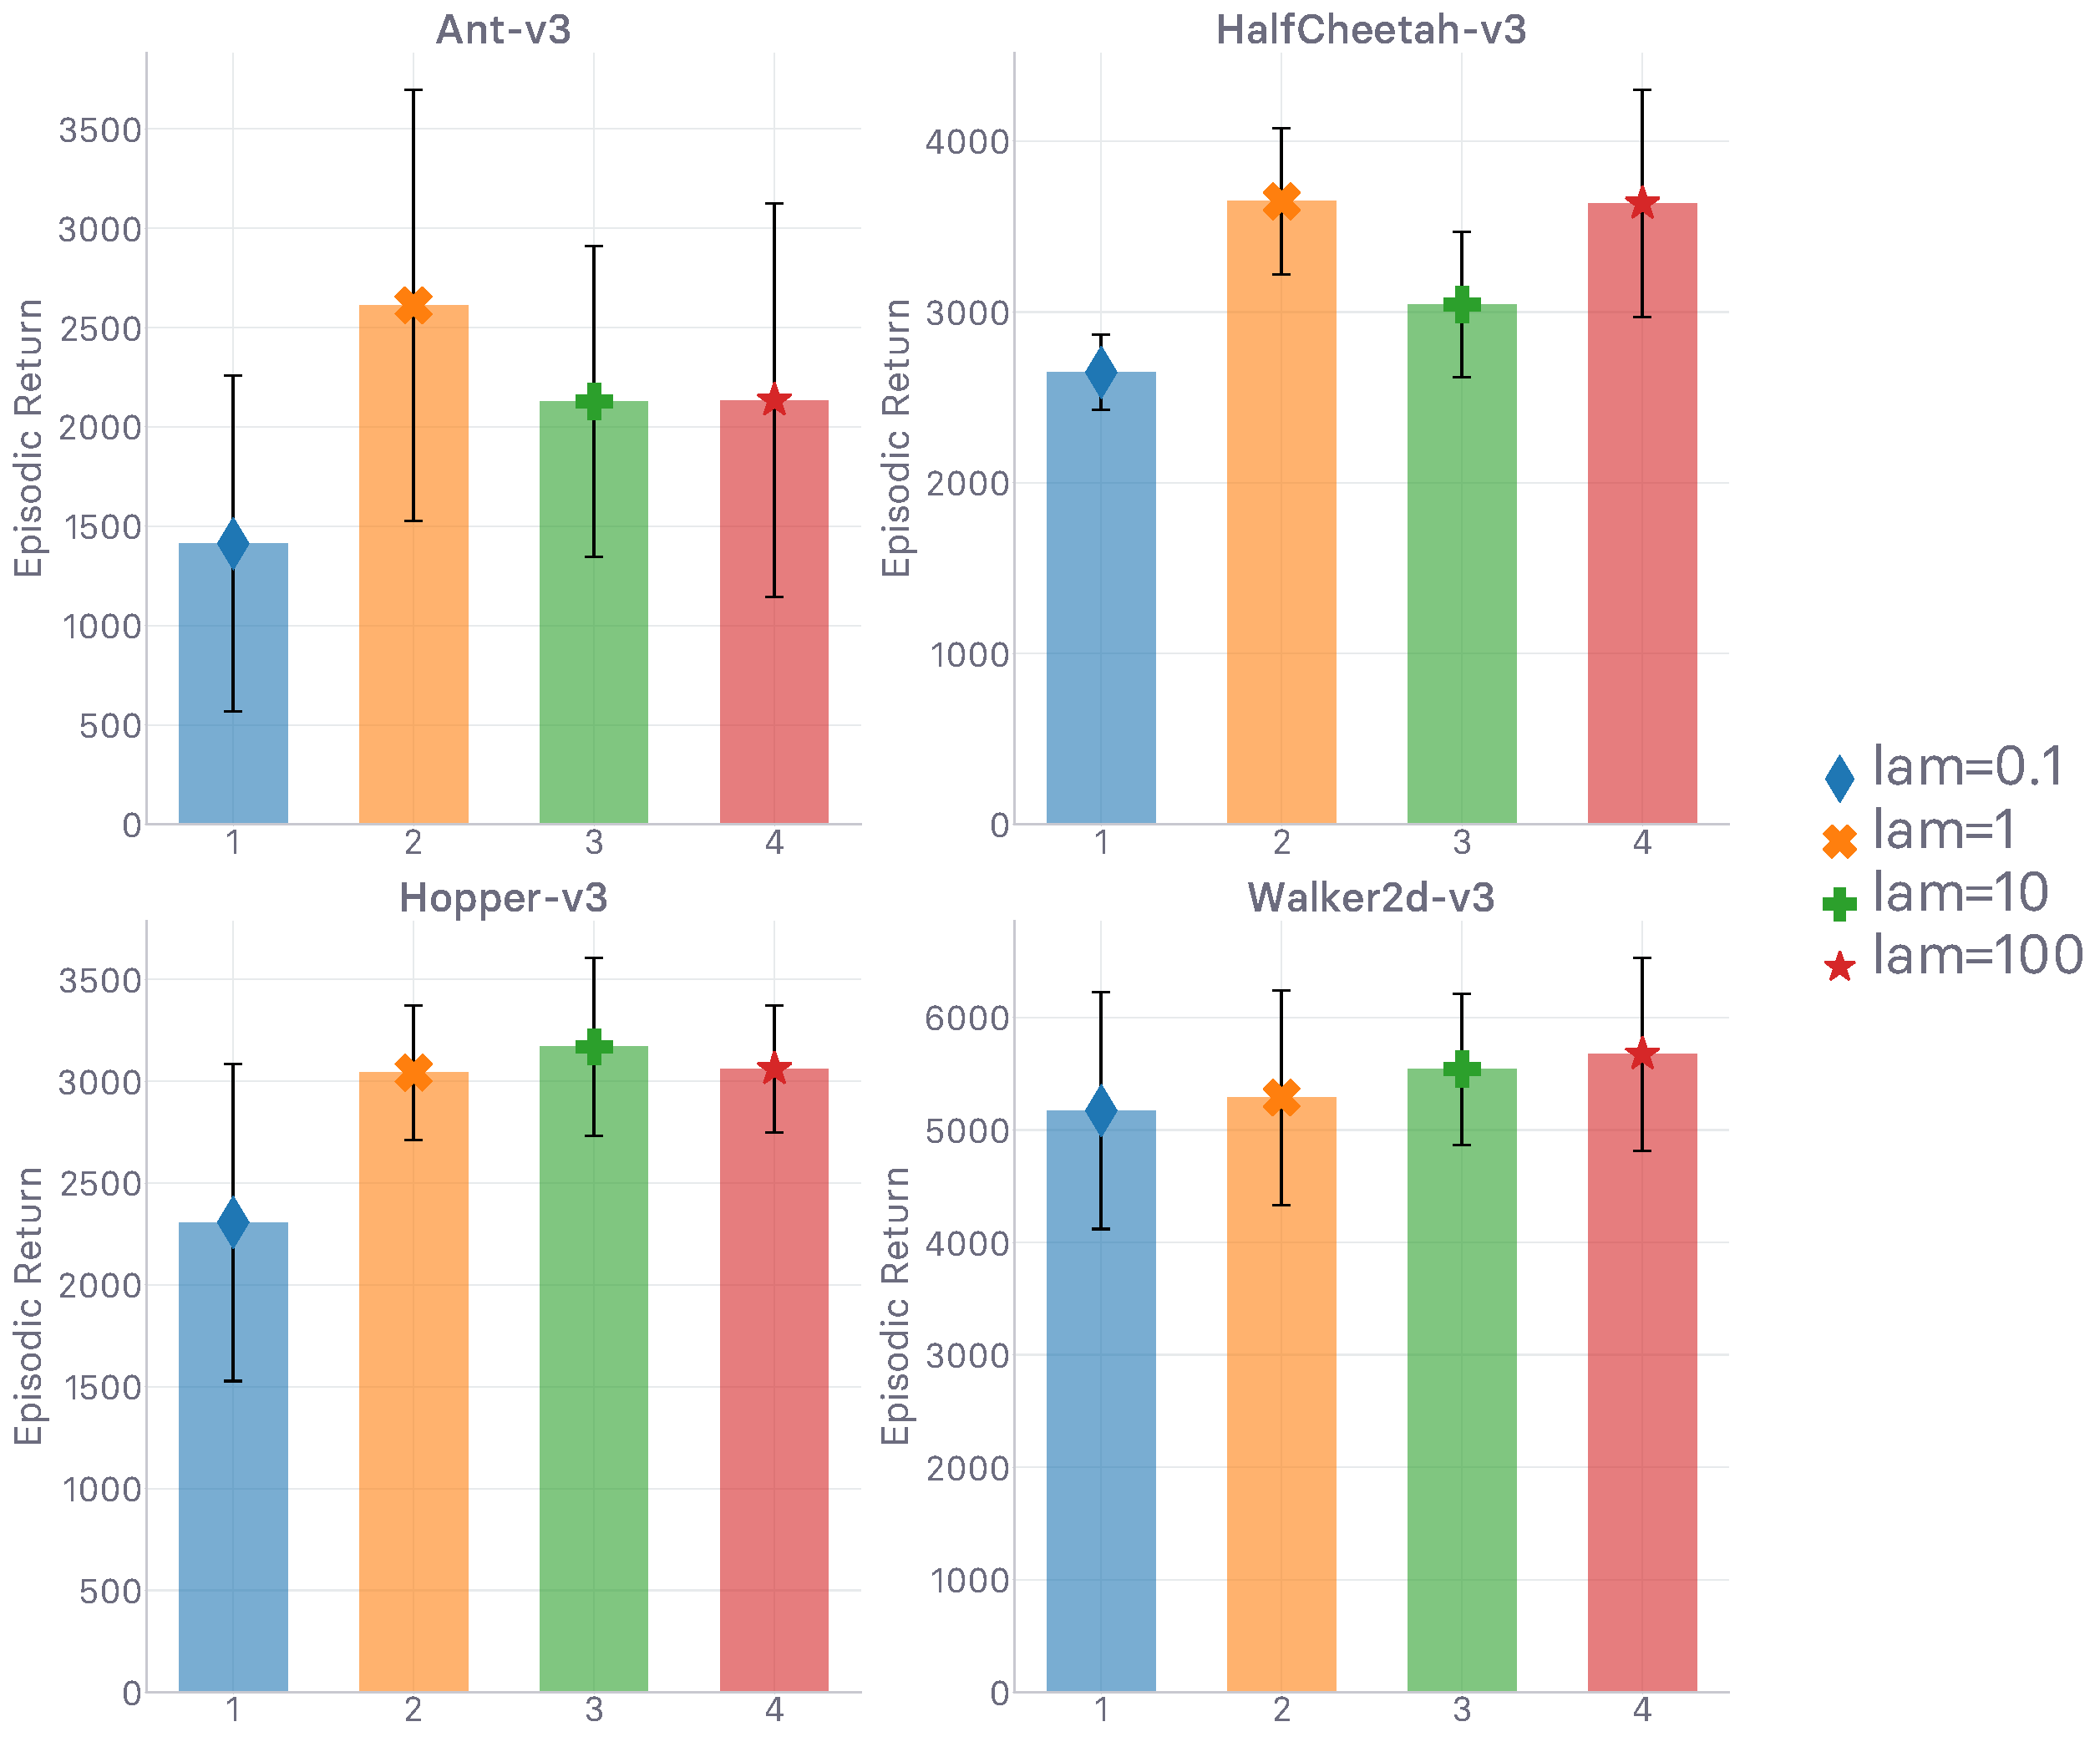
\includegraphics{Plots/fig16_k1_lam_gs_4envs/plots_eval_env_ret_barplot.pdf}}
    \caption{Final return values at timeout \textit{(higher is better)}}
  \end{subfigure}
  \caption{
  Grid search over the hyper-parameter $\lambda$ when $k=1$.
  Runtime is 12 hours.}
  \label{gridk1}
\end{figure}

\begin{figure}[H]
  \center
  \begin{subfigure}[t]{0.49\textwidth}
    \center\scalebox{0.16}[0.16]{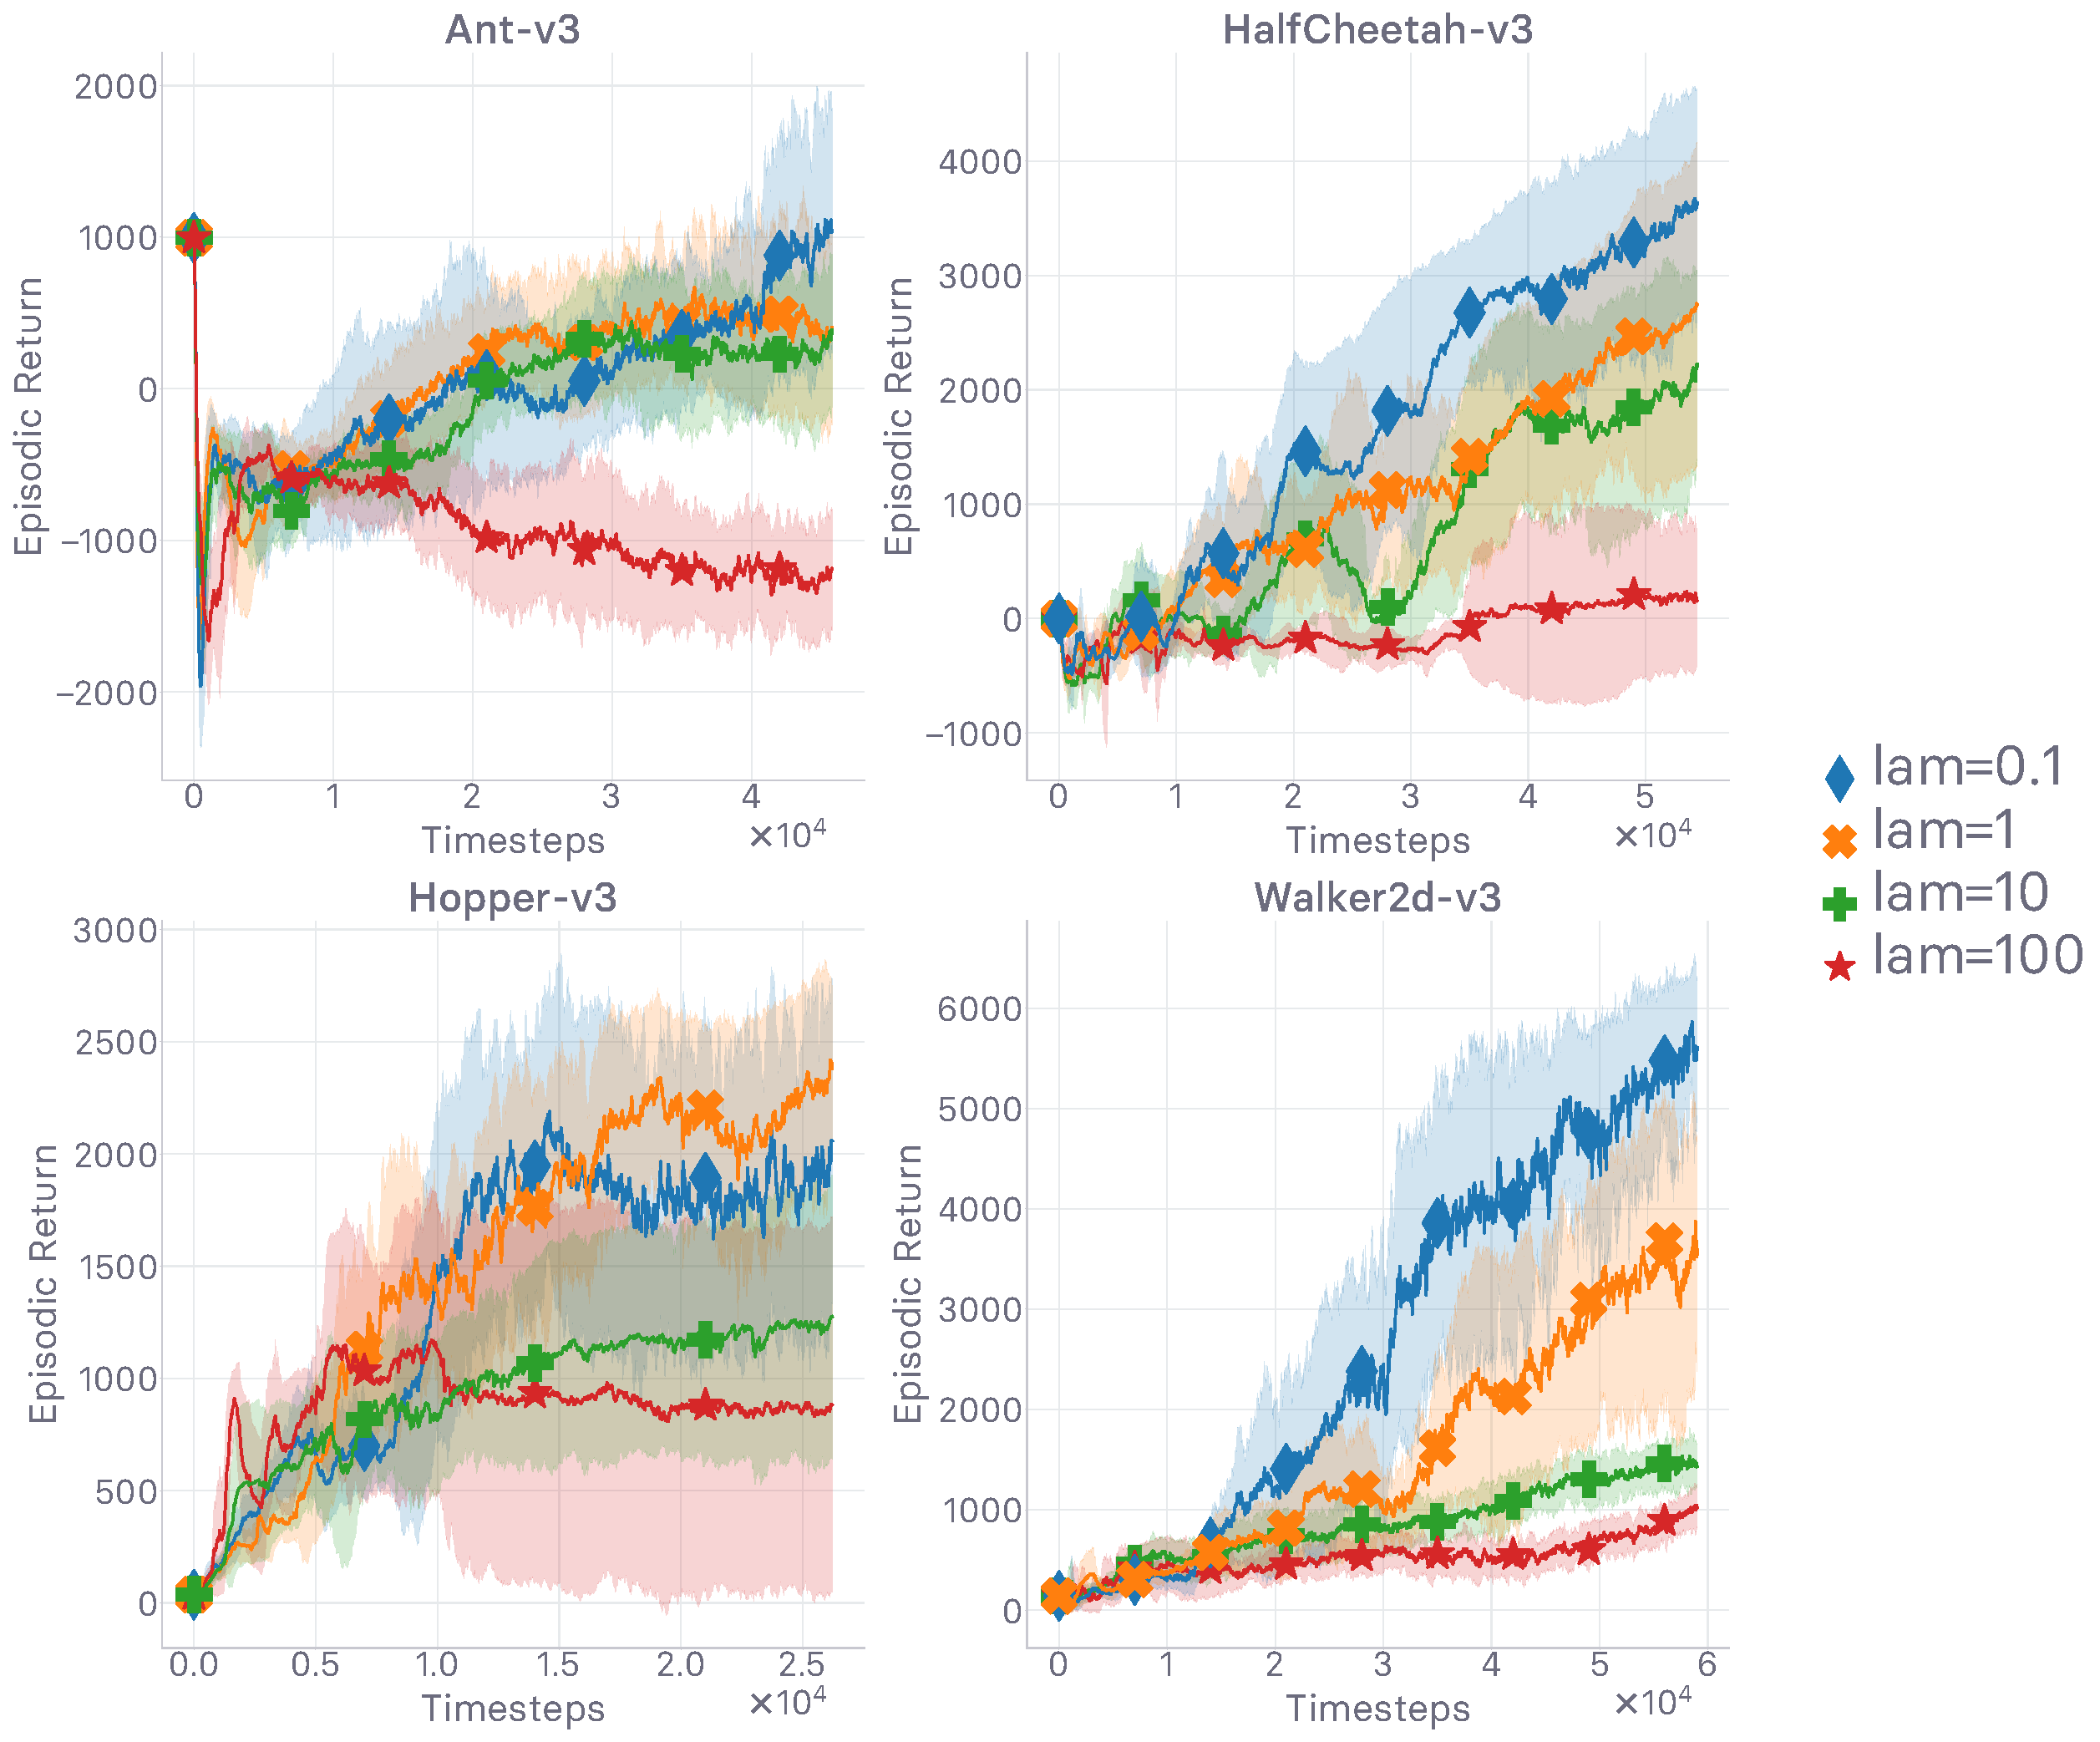
\includegraphics{Plots/fig17_k0_lam_gs_4envs/plots_eval_env_ret_plot.pdf}}
    \caption{Evolution of return values \textit{(higher is better)}}
  \end{subfigure}
  \begin{subfigure}[t]{0.49\textwidth}
    \center\scalebox{0.16}[0.16]{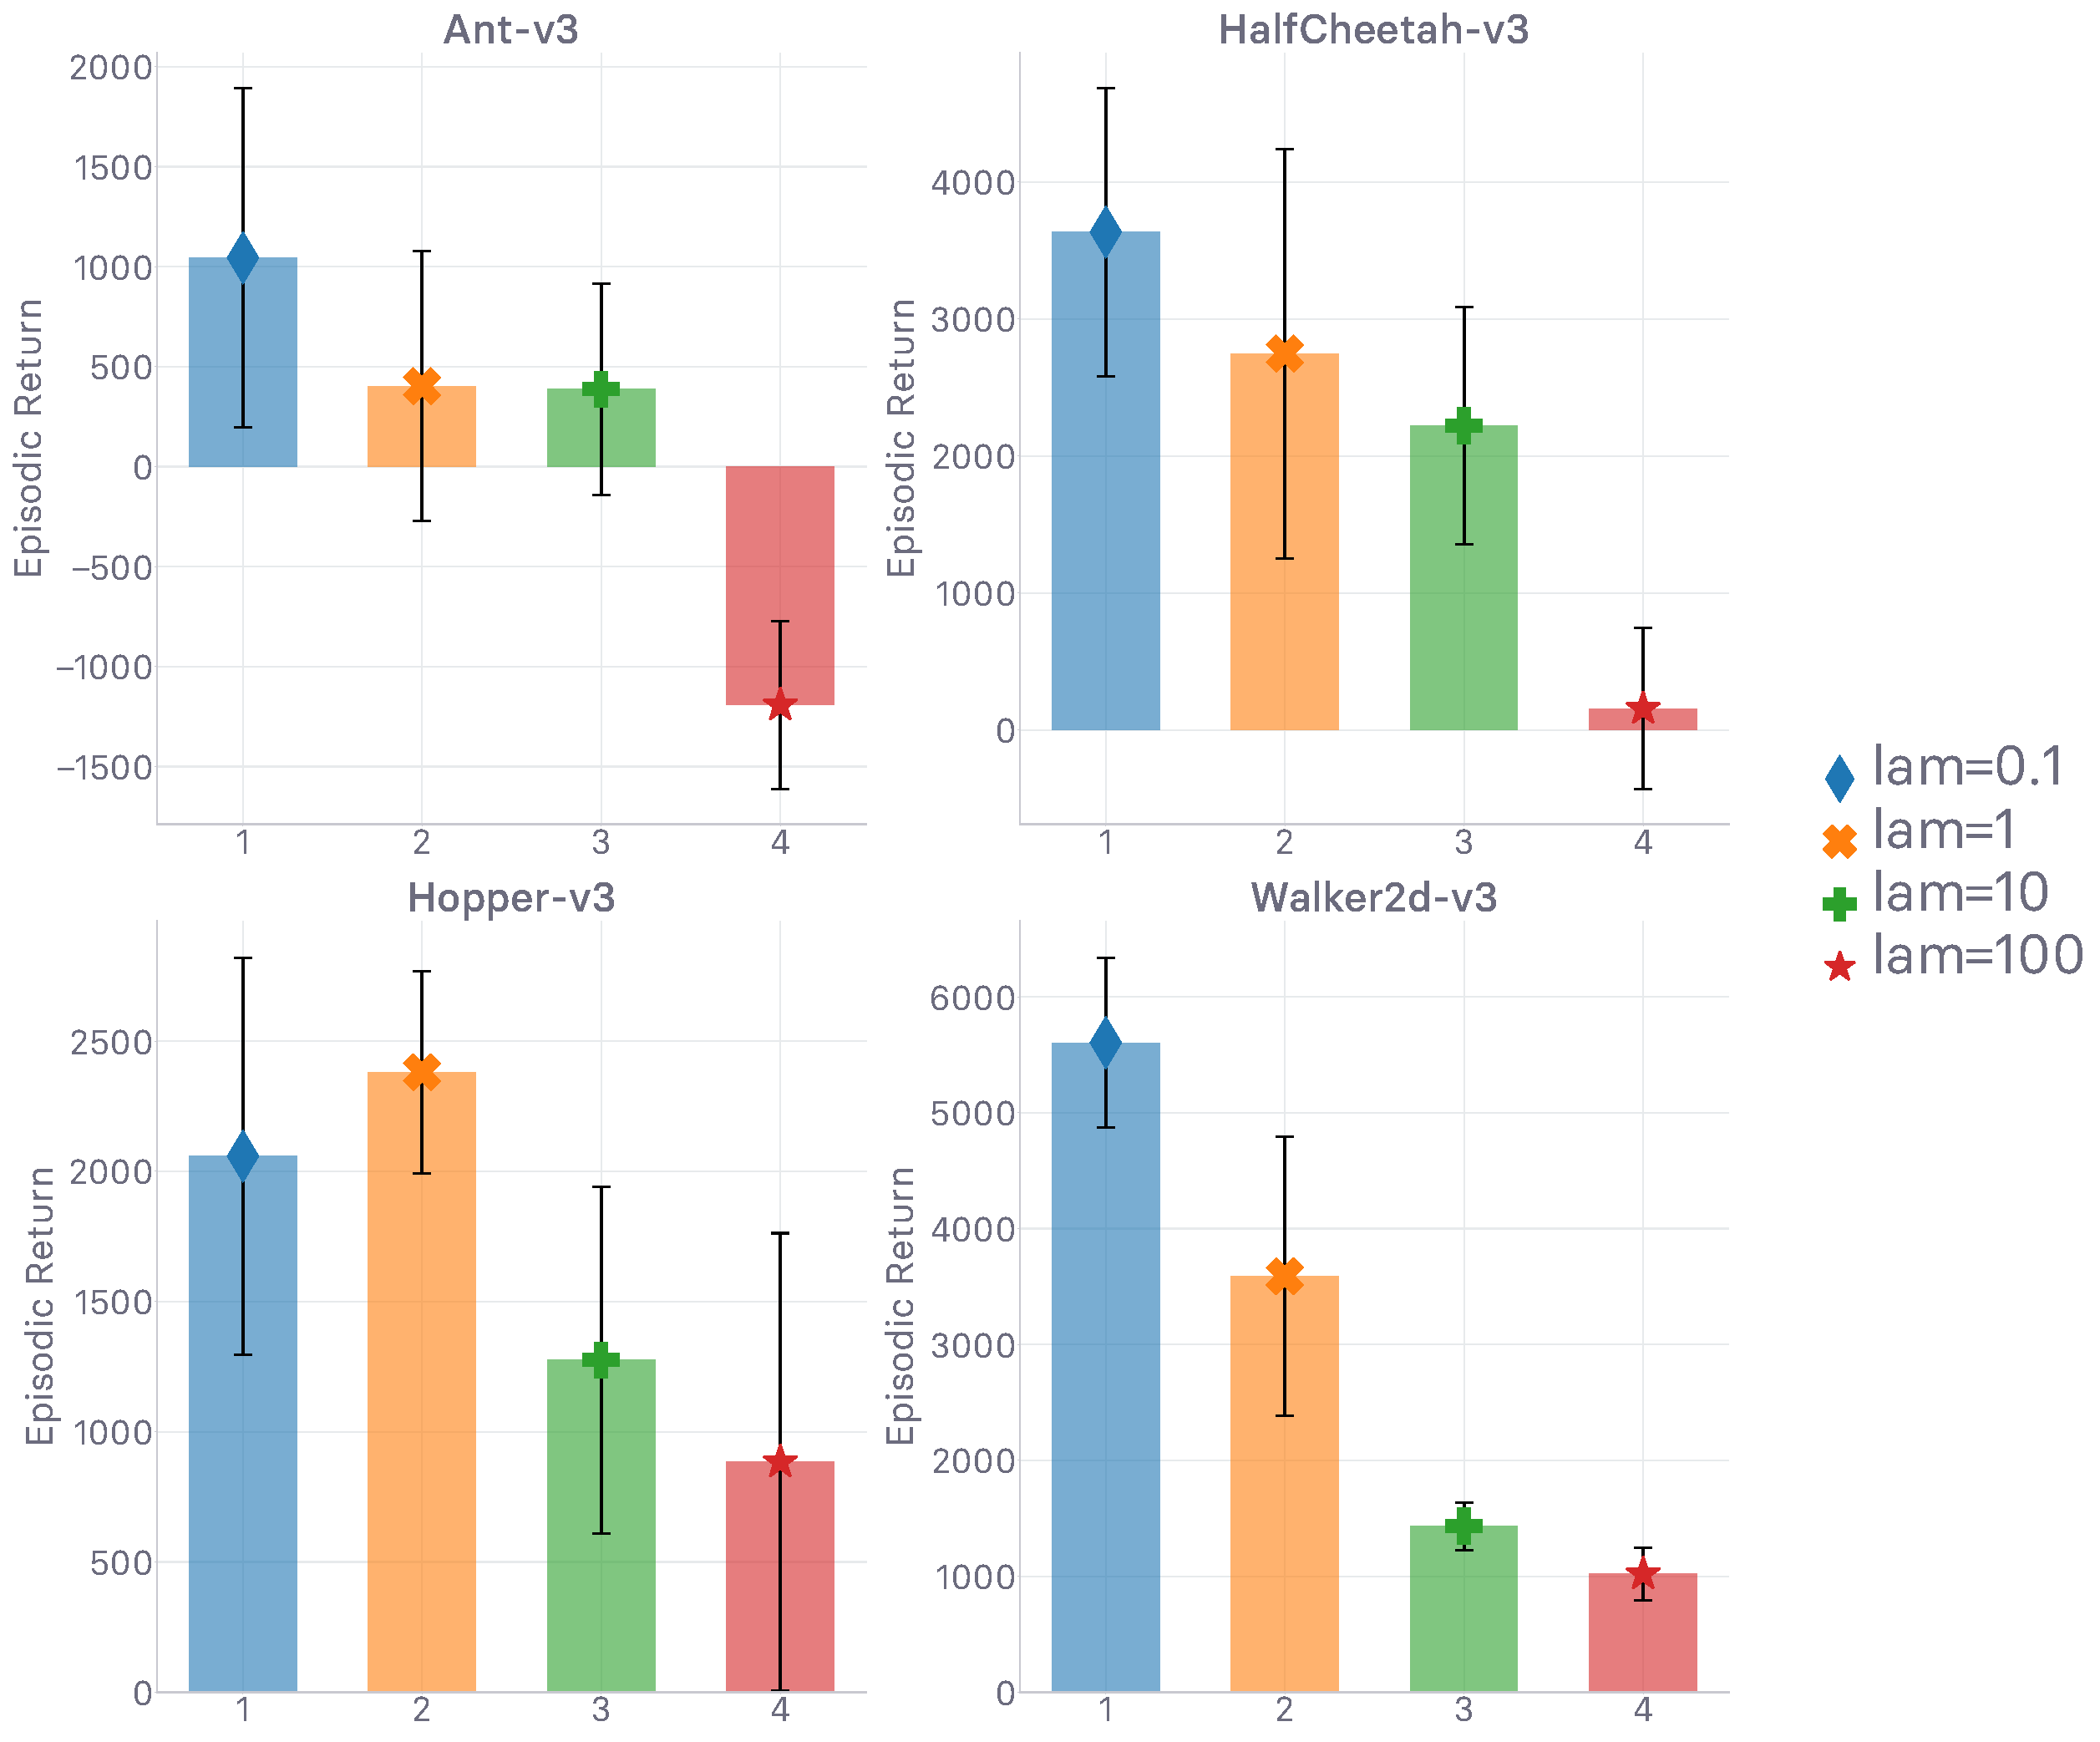
\includegraphics{Plots/fig17_k0_lam_gs_4envs/plots_eval_env_ret_barplot.pdf}}
    \caption{Final return values at timeout \textit{(higher is better)}}
  \end{subfigure}
  \caption{
  Grid search over the hyper-parameter $\lambda$ when $k=0$.
  Runtime is 12 hours.}
\end{figure}

\section{Reward Formulation}
\label{ablationreward}

\begin{figure}[H]
  \center
  \begin{subfigure}[t]{0.49\textwidth}
    \center\scalebox{0.15}[0.15]{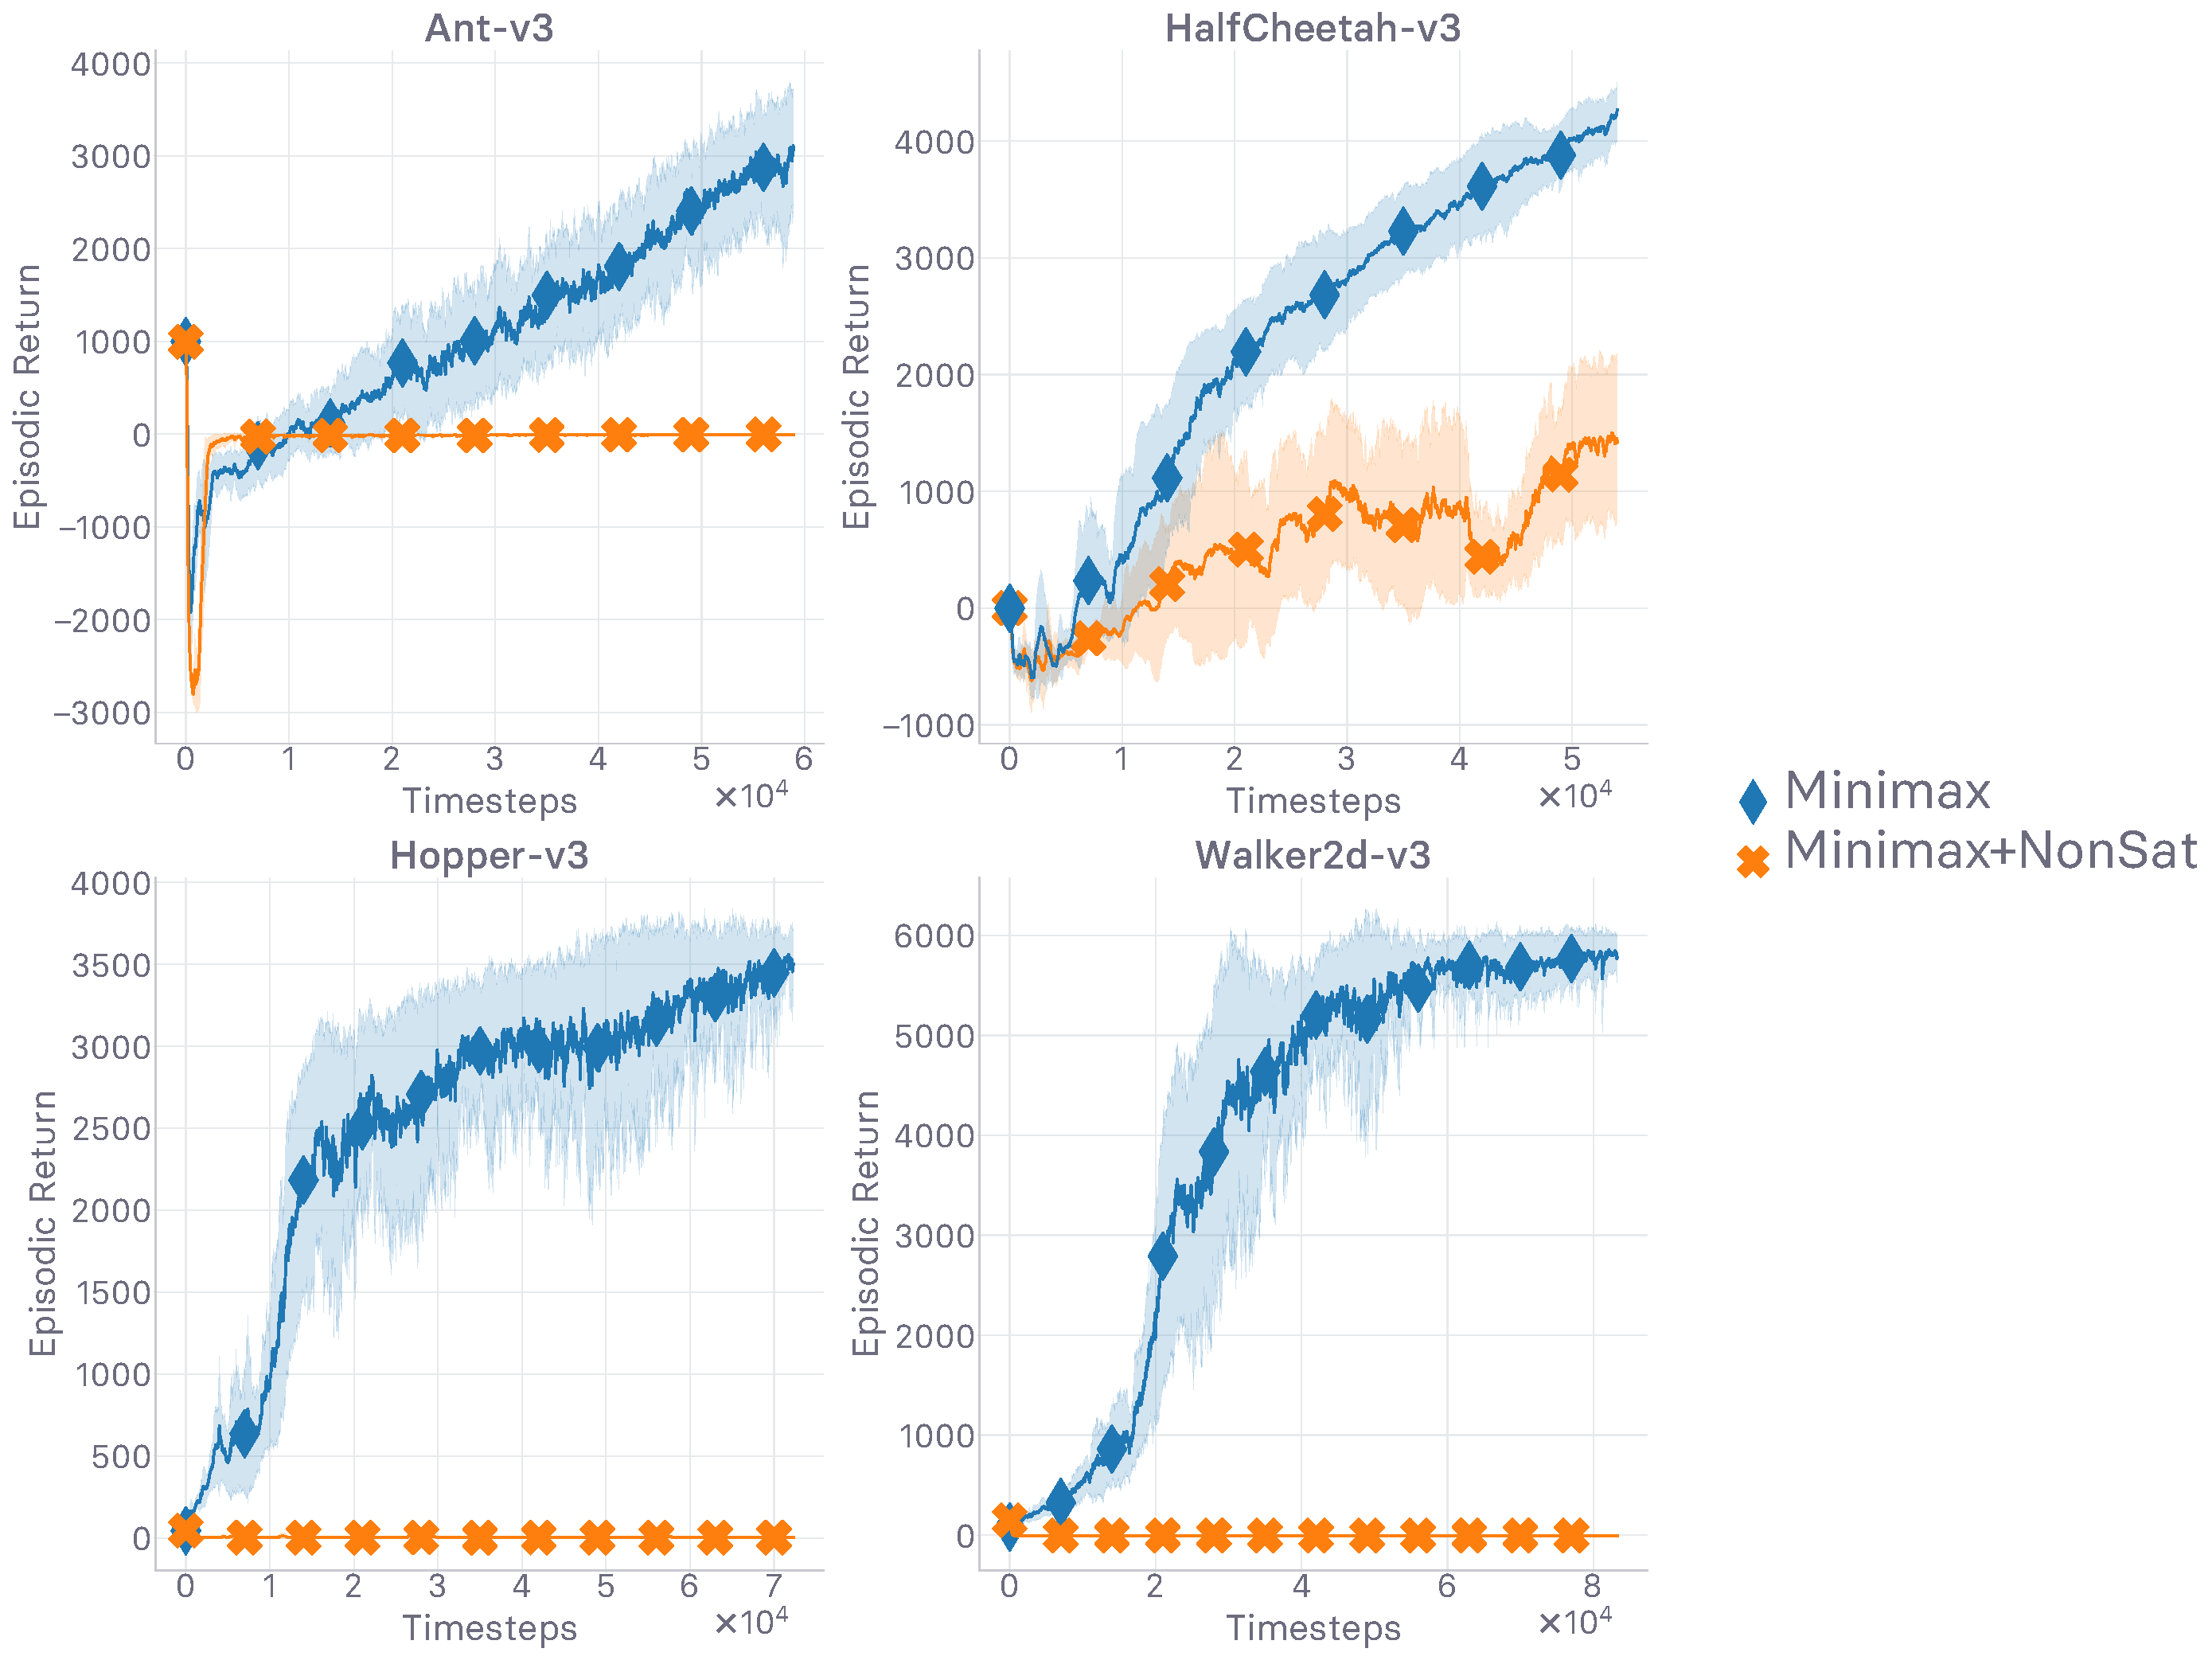
\includegraphics{Plots/fig18_minimax_4envs/plots_eval_env_ret_plot.pdf}}
    \caption{Evolution of return values \textit{(higher is better)}}
  \end{subfigure}
  \begin{subfigure}[t]{0.49\textwidth}
    \center\scalebox{0.15}[0.15]{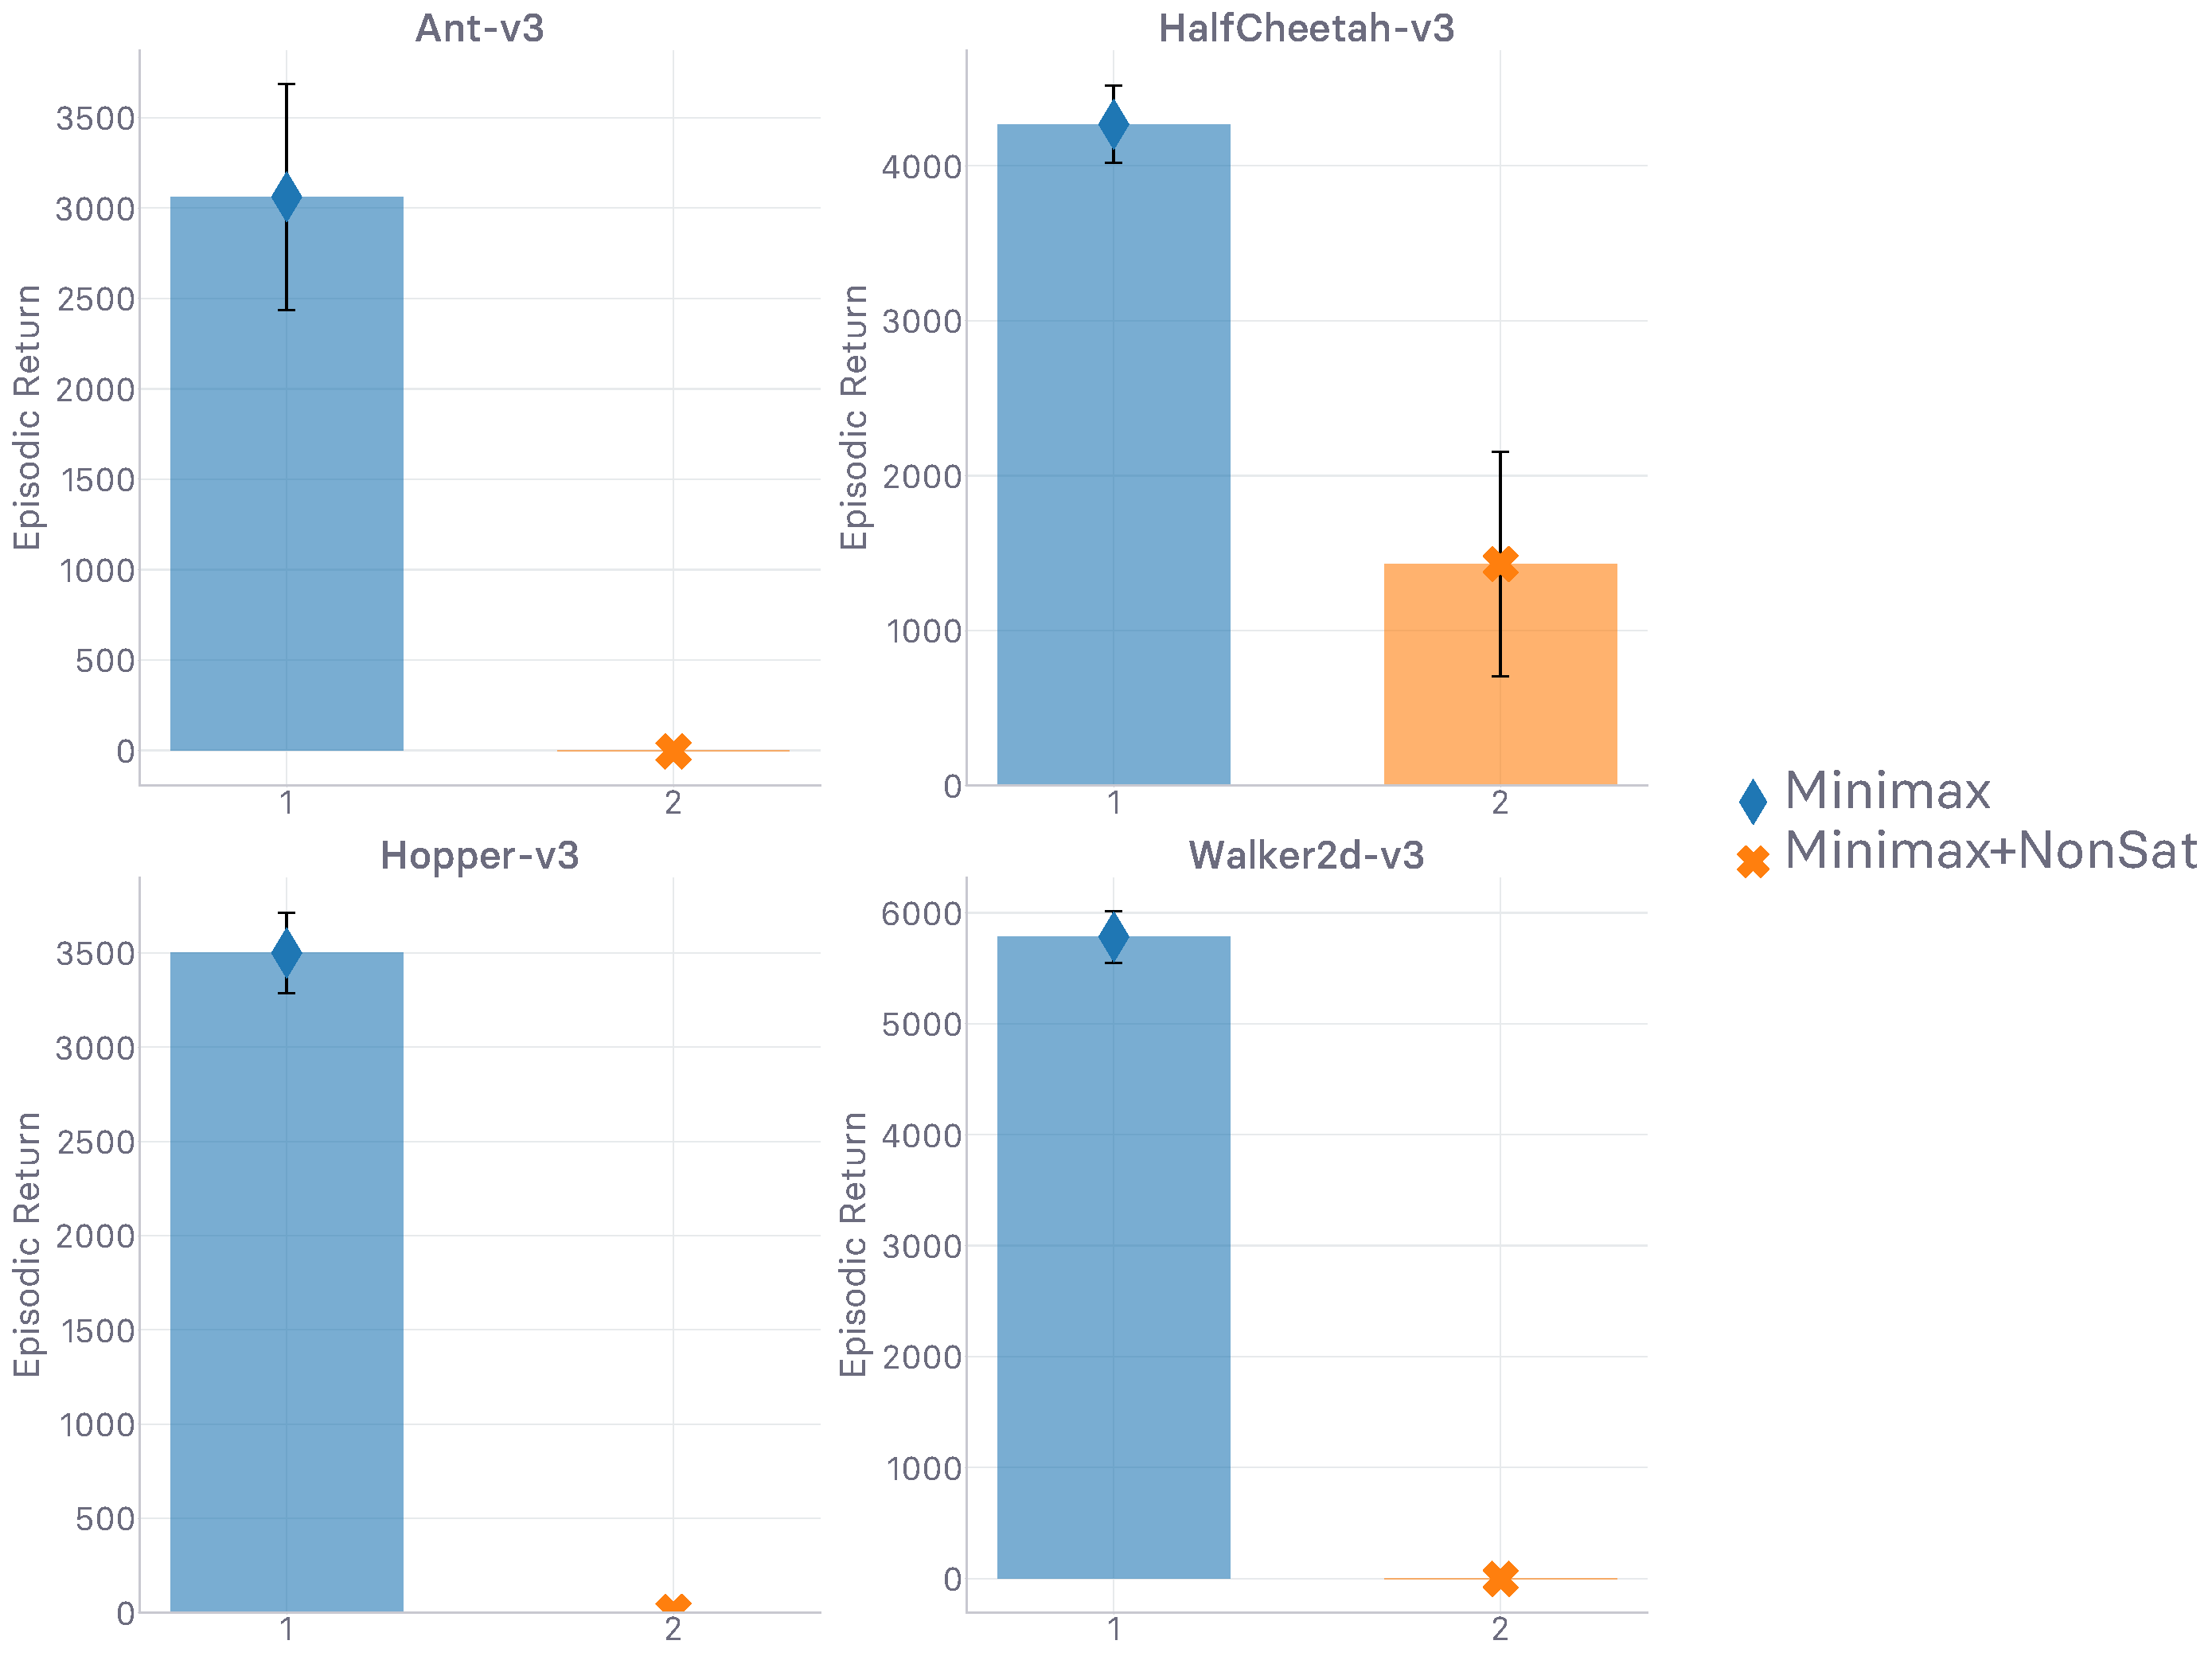
\includegraphics{Plots/fig18_minimax_4envs/plots_eval_env_ret_barplot.pdf}}
    \caption{Final return values at timeout \textit{(higher is better)}}
  \end{subfigure}
  \caption{
  Comparison of two ways to define the surrogate imitation reward $r_\varphi$
  from the discriminator $D_\varphi$.
  \textit{``Minimax''} corresponds to
  $r_\varphi^\textsc{mm} \coloneqq -\log(1-D_\varphi)$,
  while \textit{``Minimax + Non-Saturating''} denotes the use of
  $r_\varphi^\textsc{ns} \coloneqq -\log(1-D_\varphi) + \log(D_\varphi)$,
  as described in \textsc{Section}~\ref{bridge}.
  Runtime is 12 hours.}
\end{figure}

\section{Discount Factor}
\label{ablationdiscount}

\begin{figure}[H]
  \center
  \begin{subfigure}[t]{0.49\textwidth}
    \center\scalebox{0.15}[0.15]{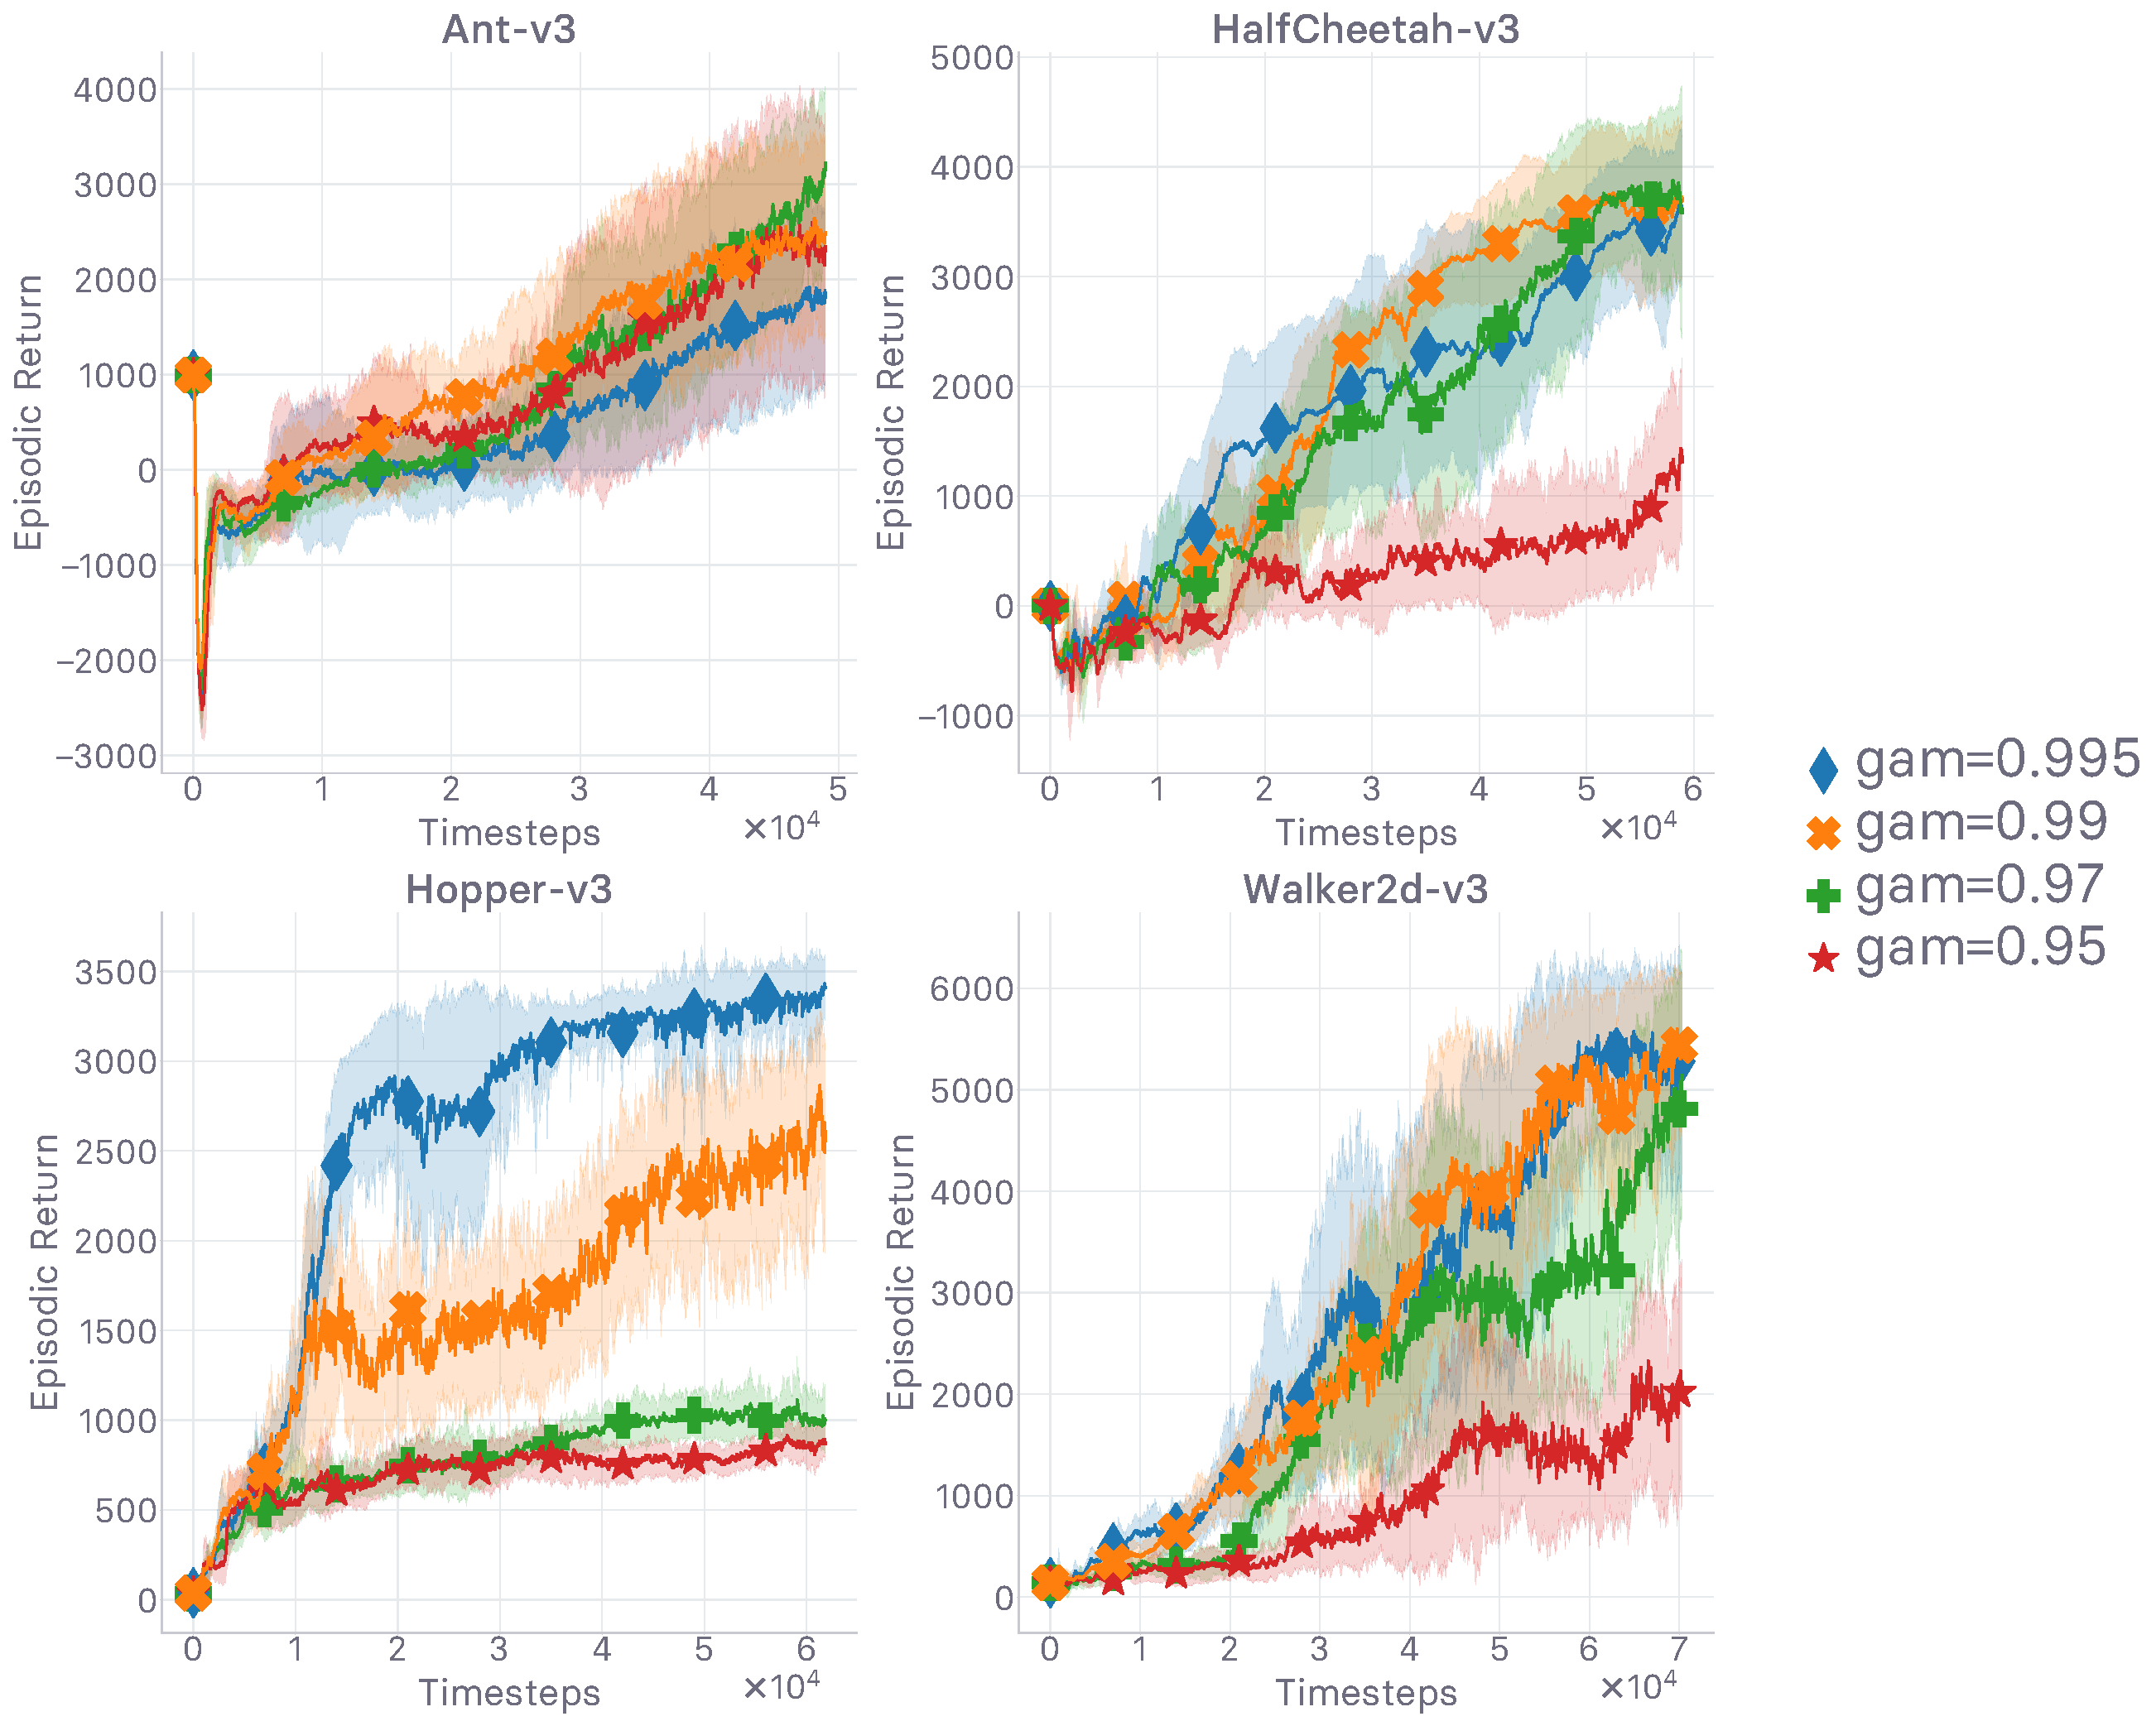
\includegraphics{Plots/fig19_discount_gs_4envs/plots_eval_env_ret_plot.pdf}}
    \caption{Evolution of return values \textit{(higher is better)}}
  \end{subfigure}
  \begin{subfigure}[t]{0.49\textwidth}
    \center\scalebox{0.15}[0.15]{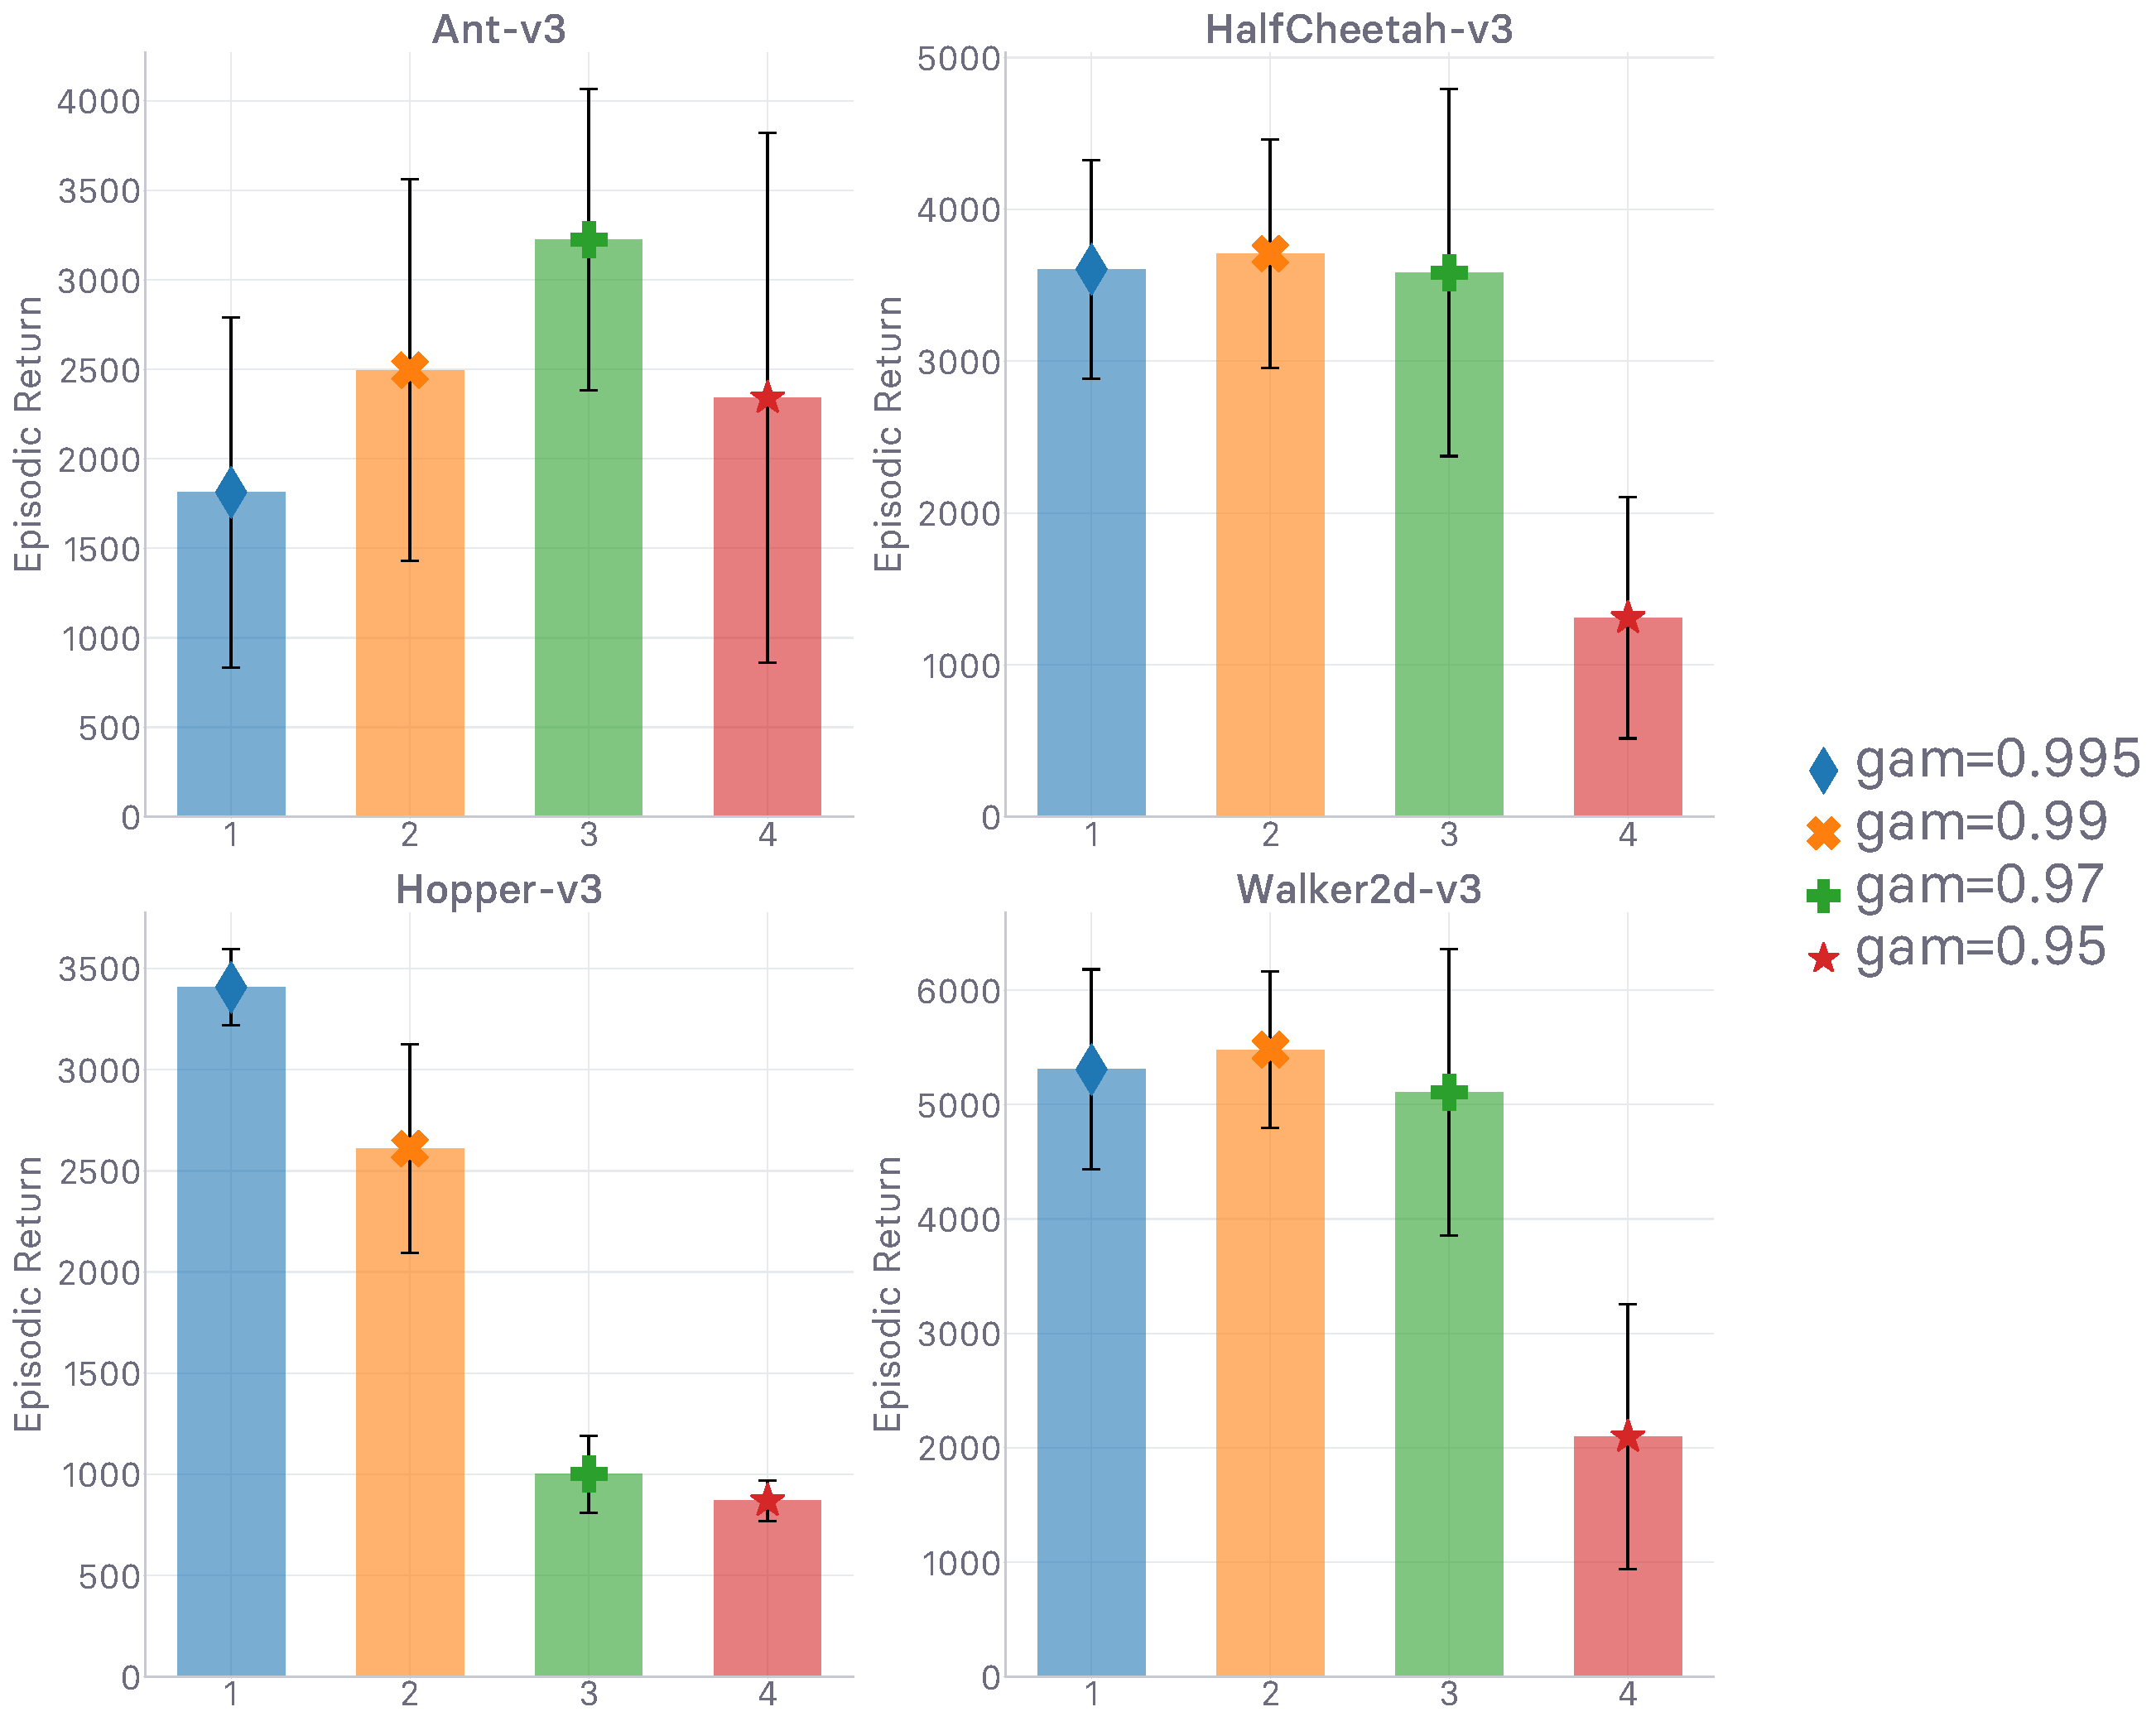
\includegraphics{Plots/fig19_discount_gs_4envs/plots_eval_env_ret_barplot.pdf}}
    \caption{Final return values at timeout \textit{(higher is better)}}
  \end{subfigure}
  \caption{
  Grid search over the discount factor $\gamma$.
  Runtime is 12 hours.}
\end{figure}

\section{Return Normalization}
\label{ablationretnorm}

\begin{figure}[H]
  \center
  \begin{subfigure}[t]{0.49\textwidth}
    \center\scalebox{0.15}[0.15]{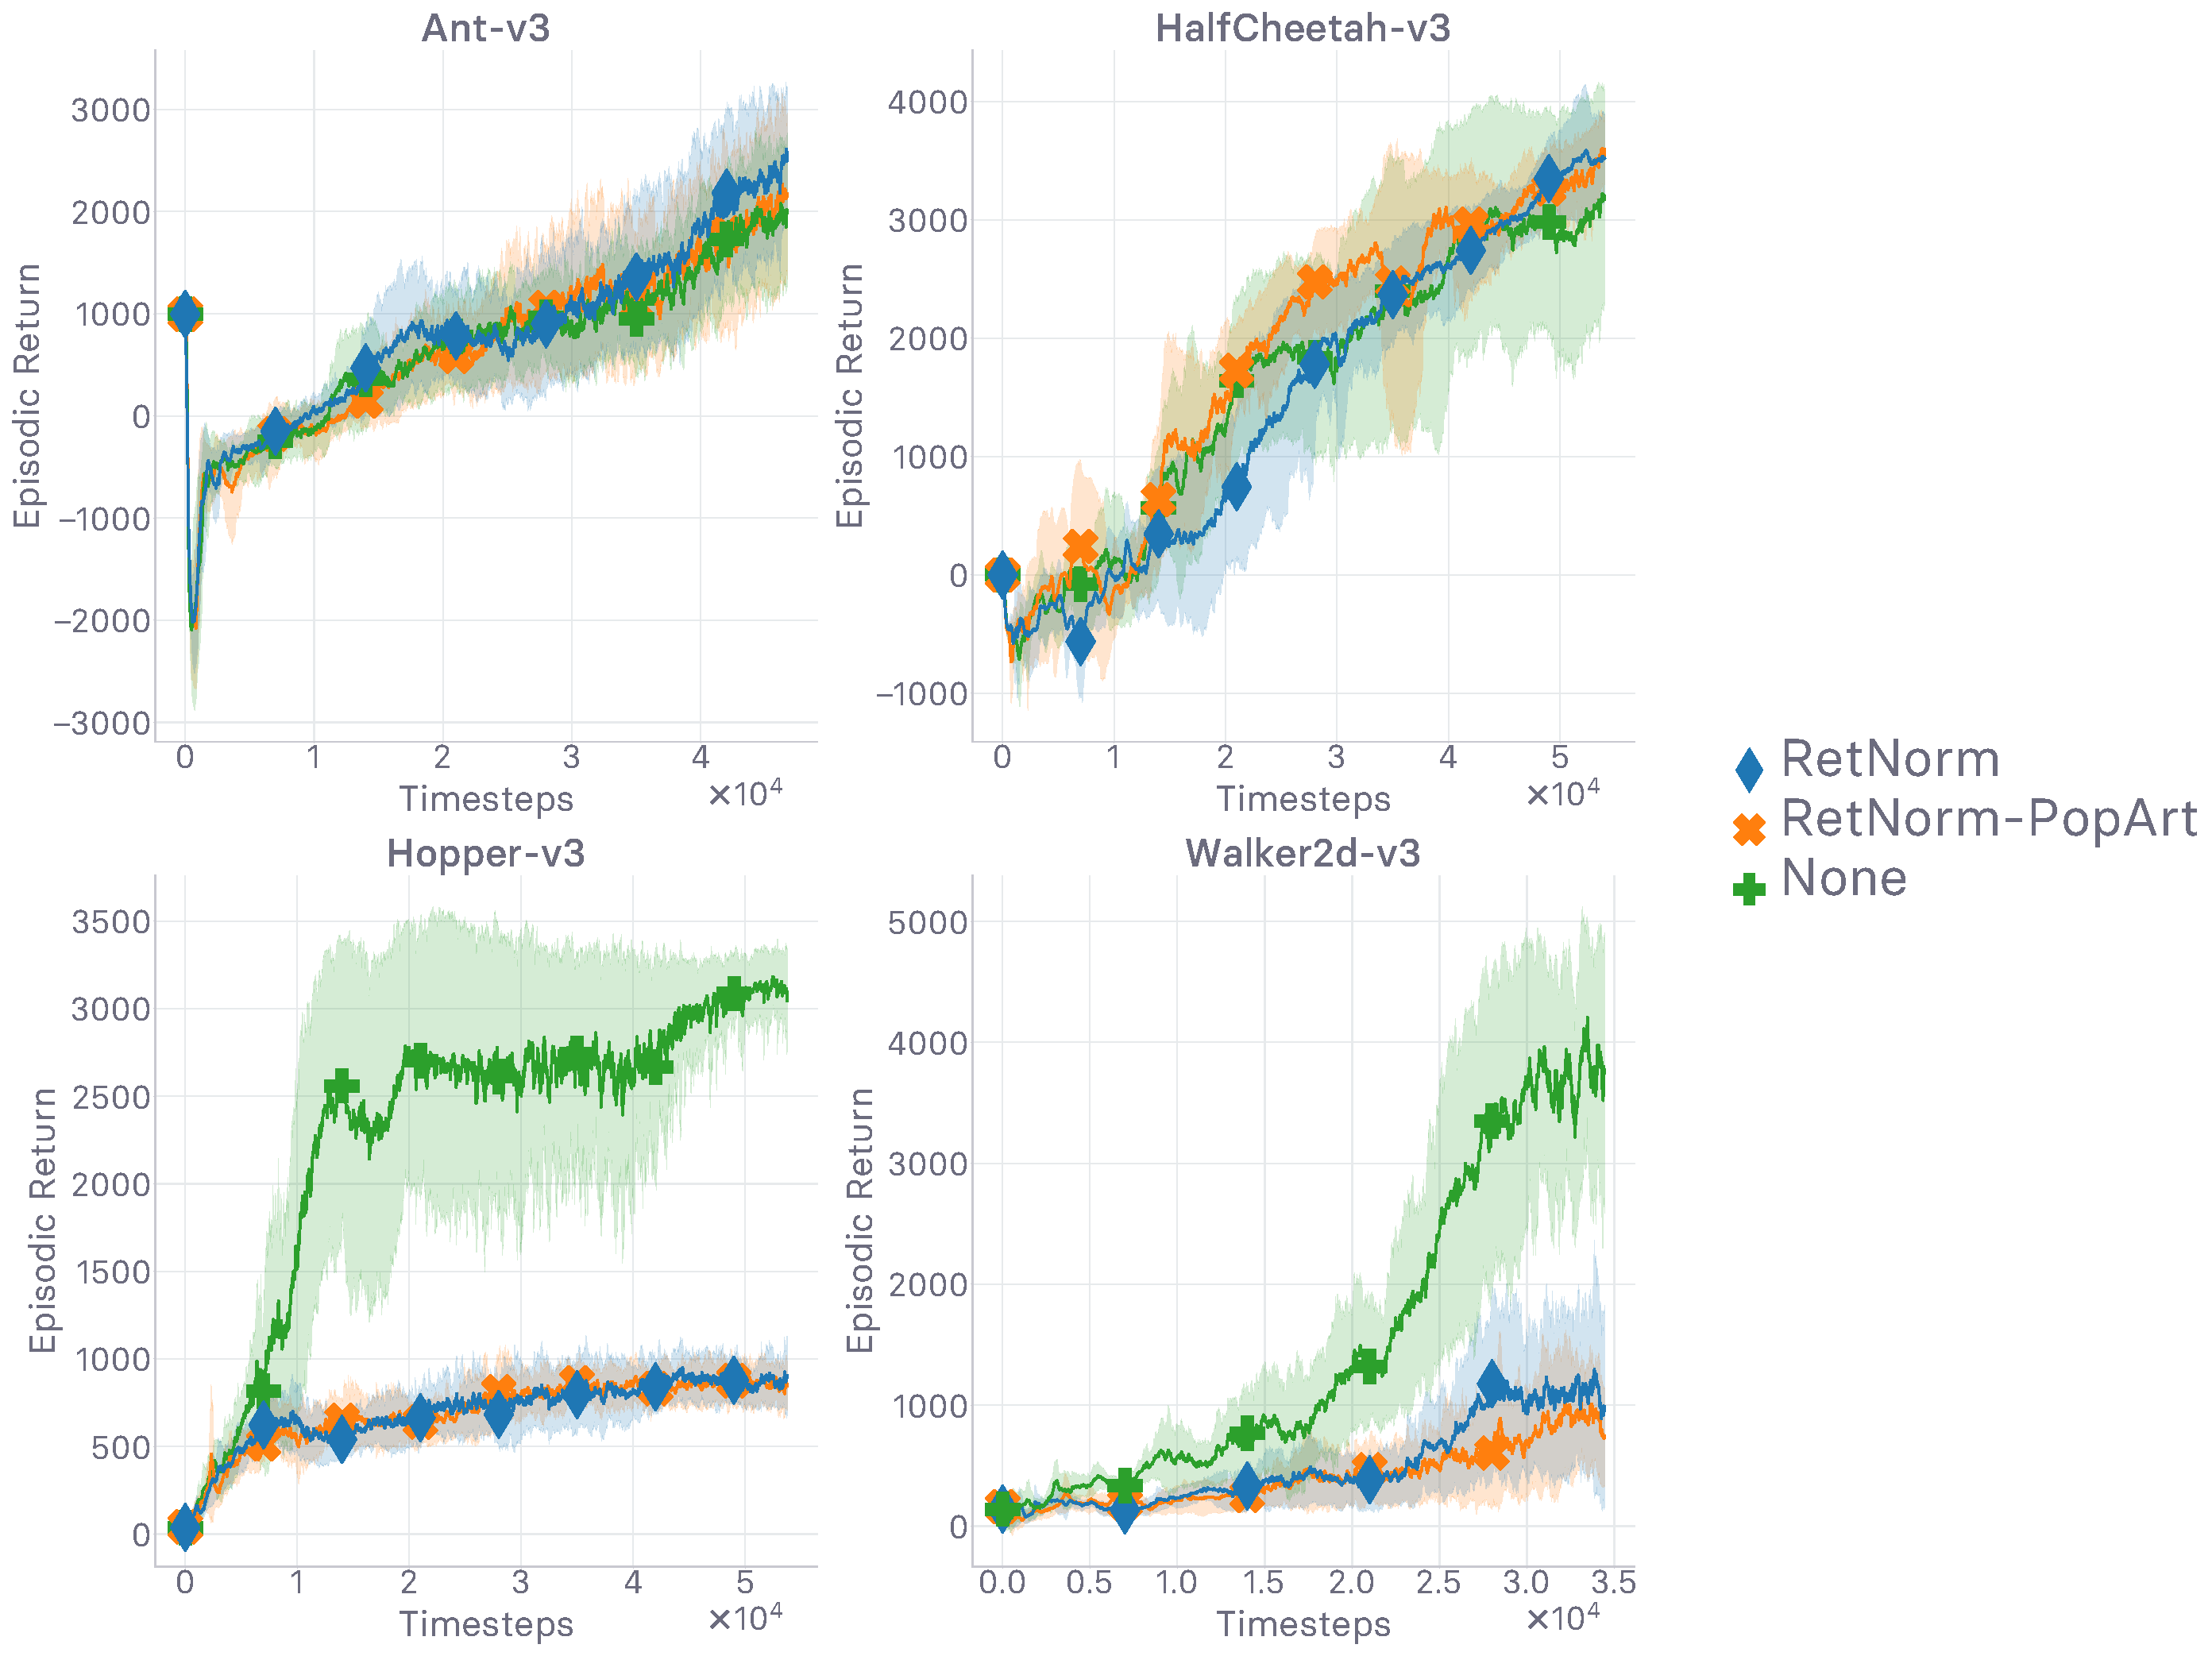
\includegraphics{Plots/fig20_retnorm_ablation_4envs/plots_eval_env_ret_plot.pdf}}
    \caption{Evolution of return values \textit{(higher is better)}}
  \end{subfigure}
  \begin{subfigure}[t]{0.49\textwidth}
    \center\scalebox{0.15}[0.15]{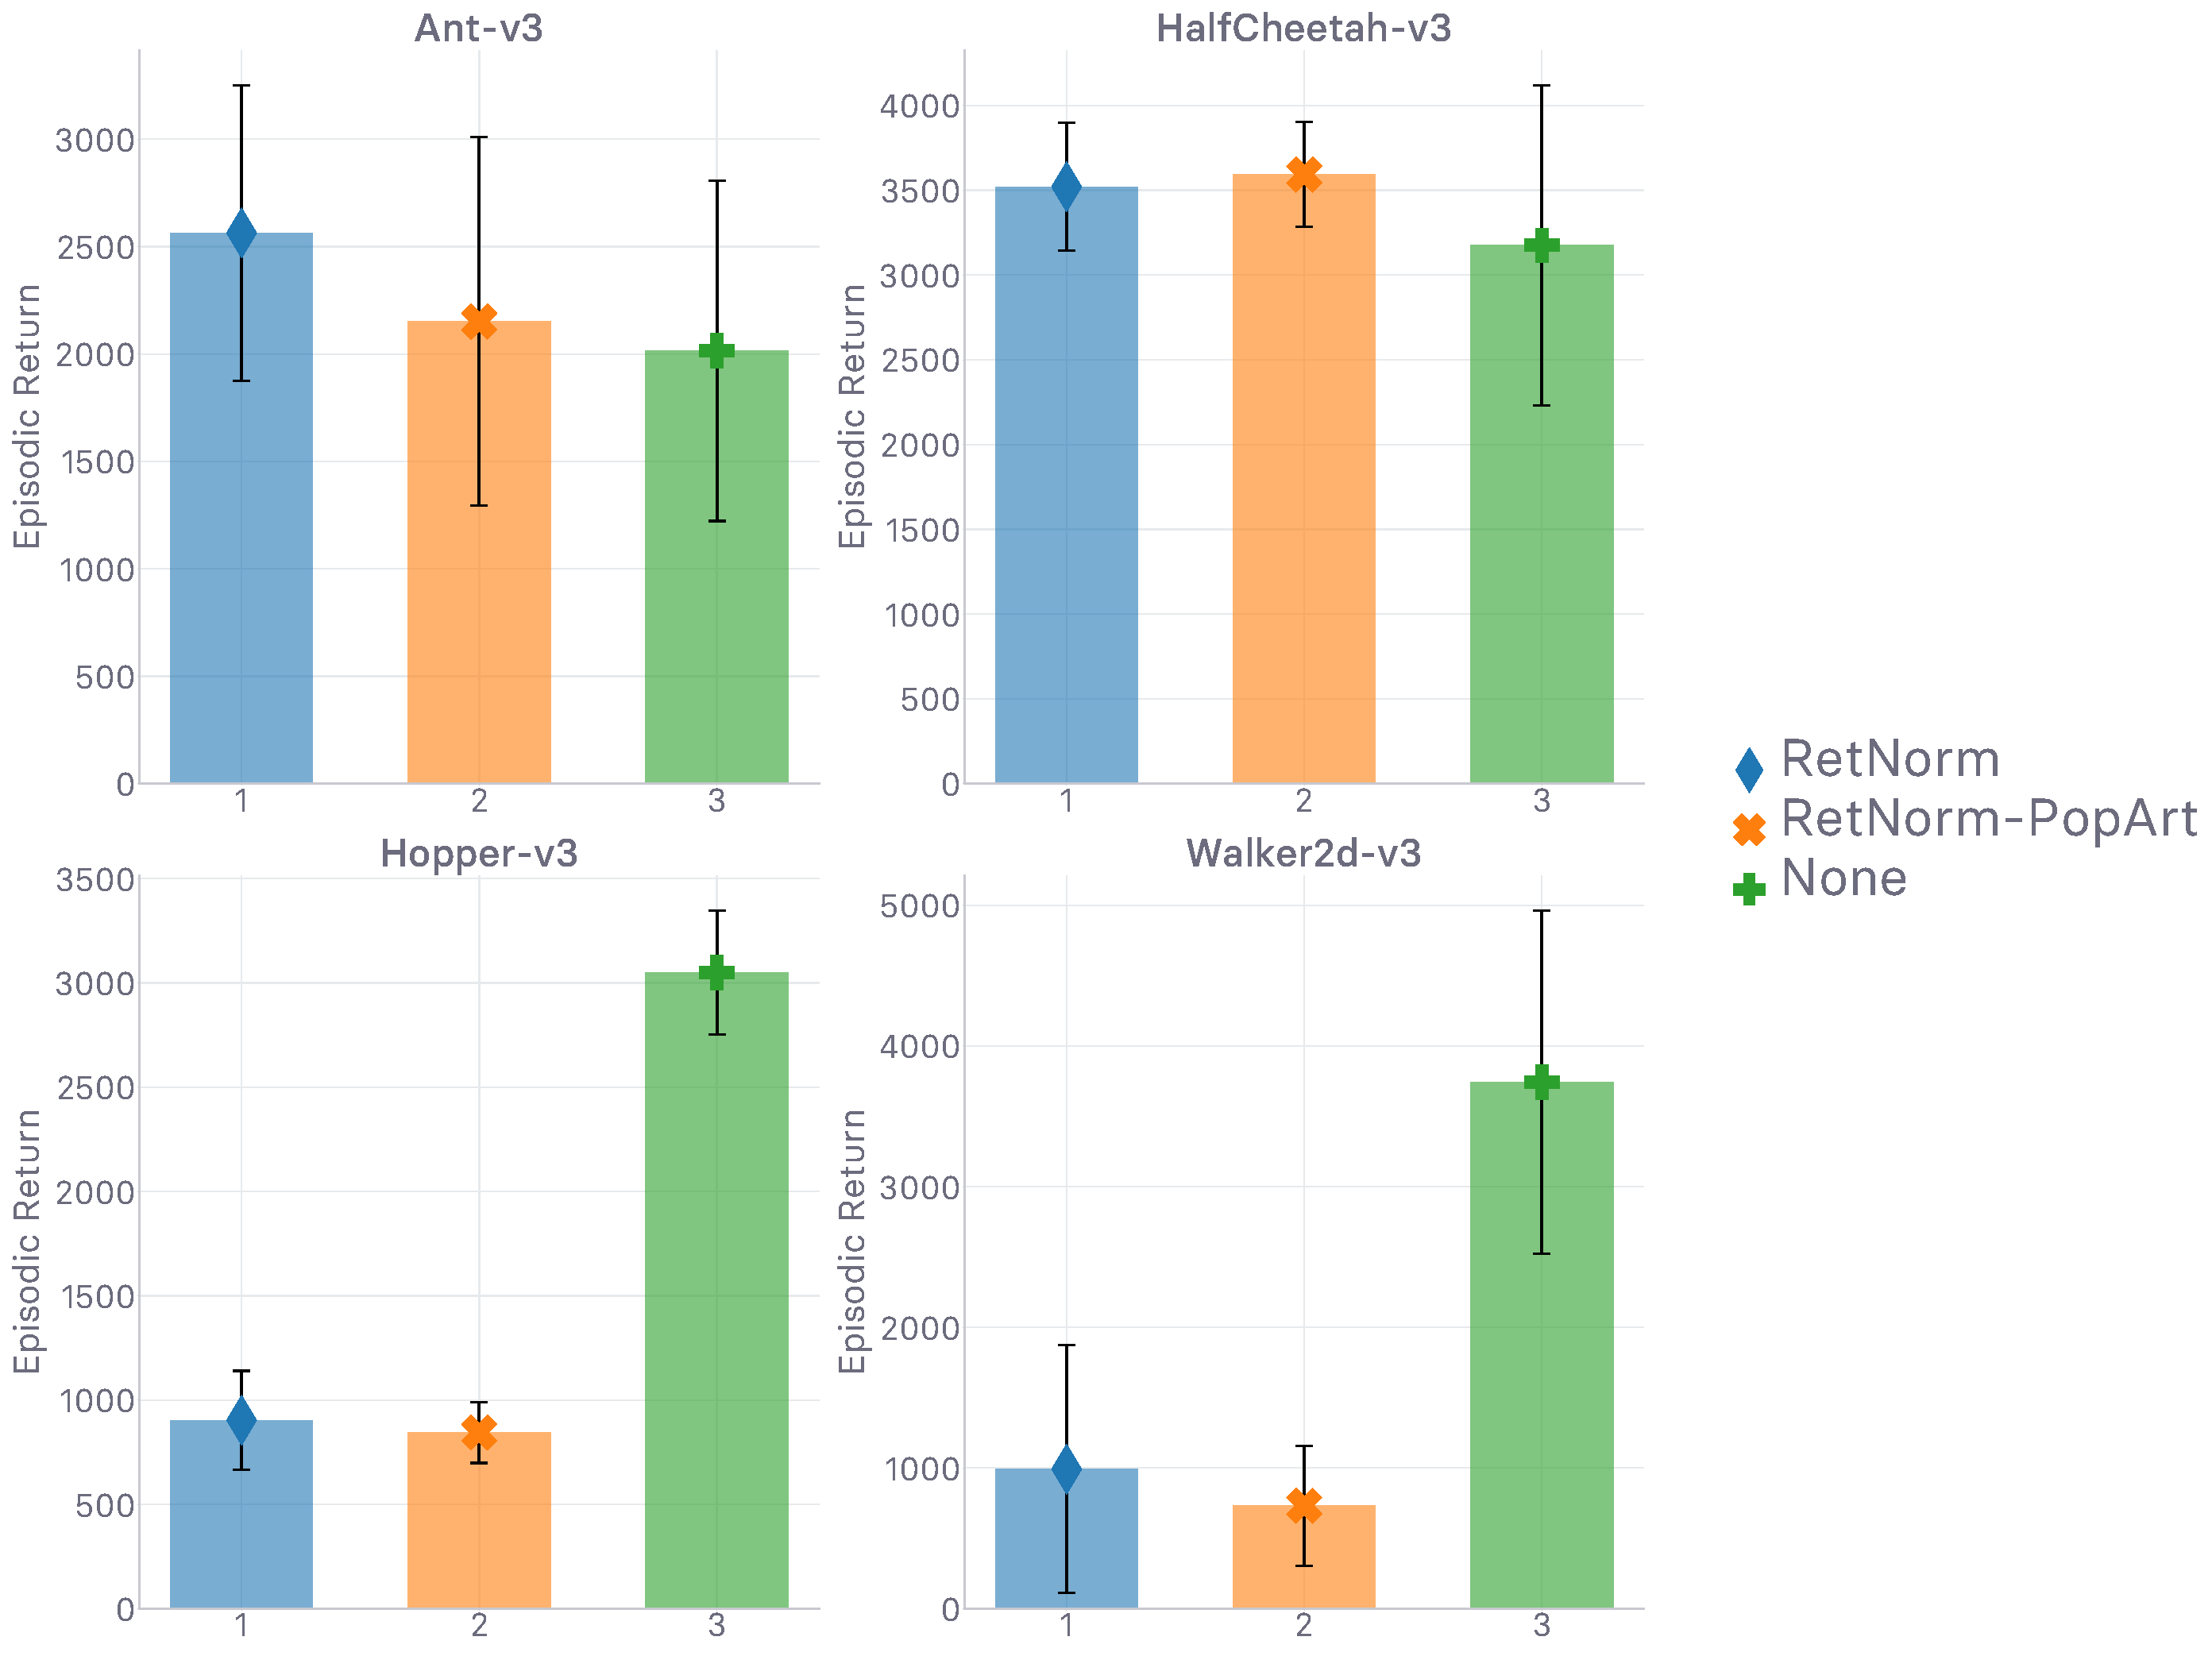
\includegraphics{Plots/fig20_retnorm_ablation_4envs/plots_eval_env_ret_barplot.pdf}}
    \caption{Final return values at timeout \textit{(higher is better)}}
  \end{subfigure}
  \caption{
  Ablation study on return normalization and \textsc{Pop-Art} \cite{Van_Hasselt2016-bh}.
  Runtime is 12 hours.}
\end{figure}

\section{Exploration}
\label{ablationexplo}

\begin{figure}[H]
  \center
  \begin{subfigure}[t]{0.49\textwidth}
    \center\scalebox{0.15}[0.15]{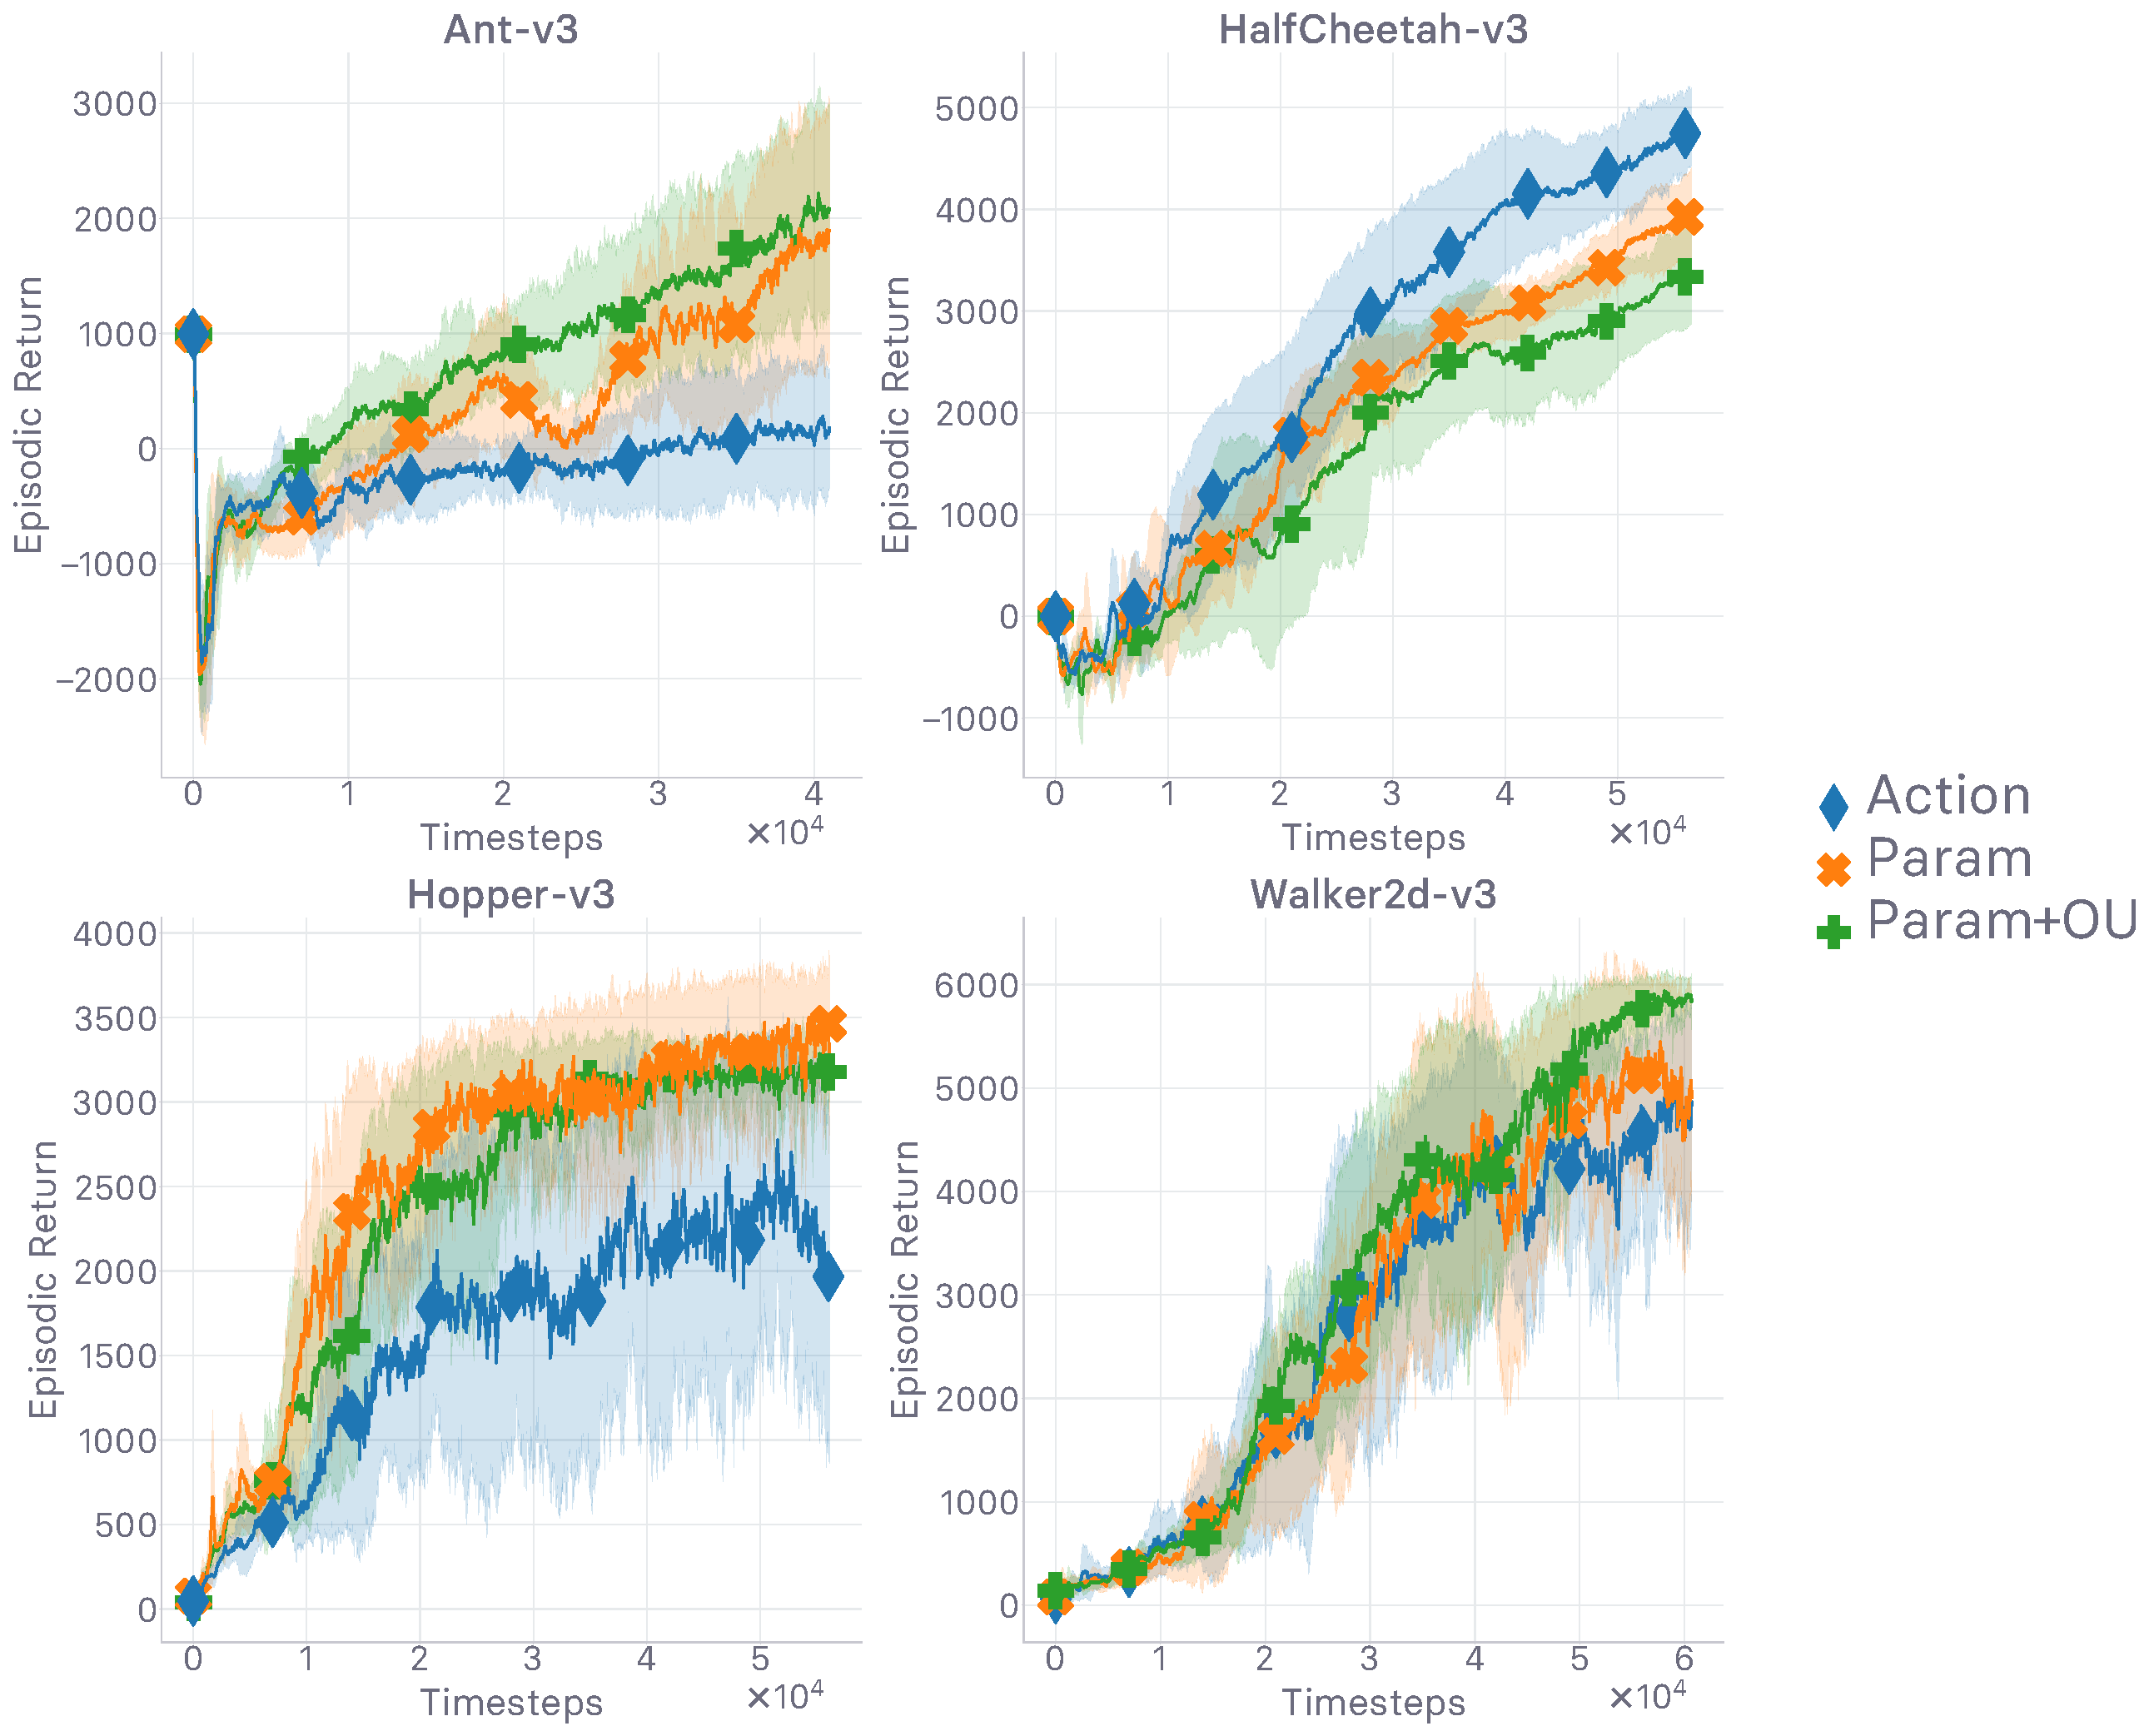
\includegraphics{Plots/fig21_explo_ablation_4envs/plots_eval_env_ret_plot.pdf}}
    \caption{Evolution of return values \textit{(higher is better)}}
  \end{subfigure}
  \begin{subfigure}[t]{0.49\textwidth}
    \center\scalebox{0.15}[0.15]{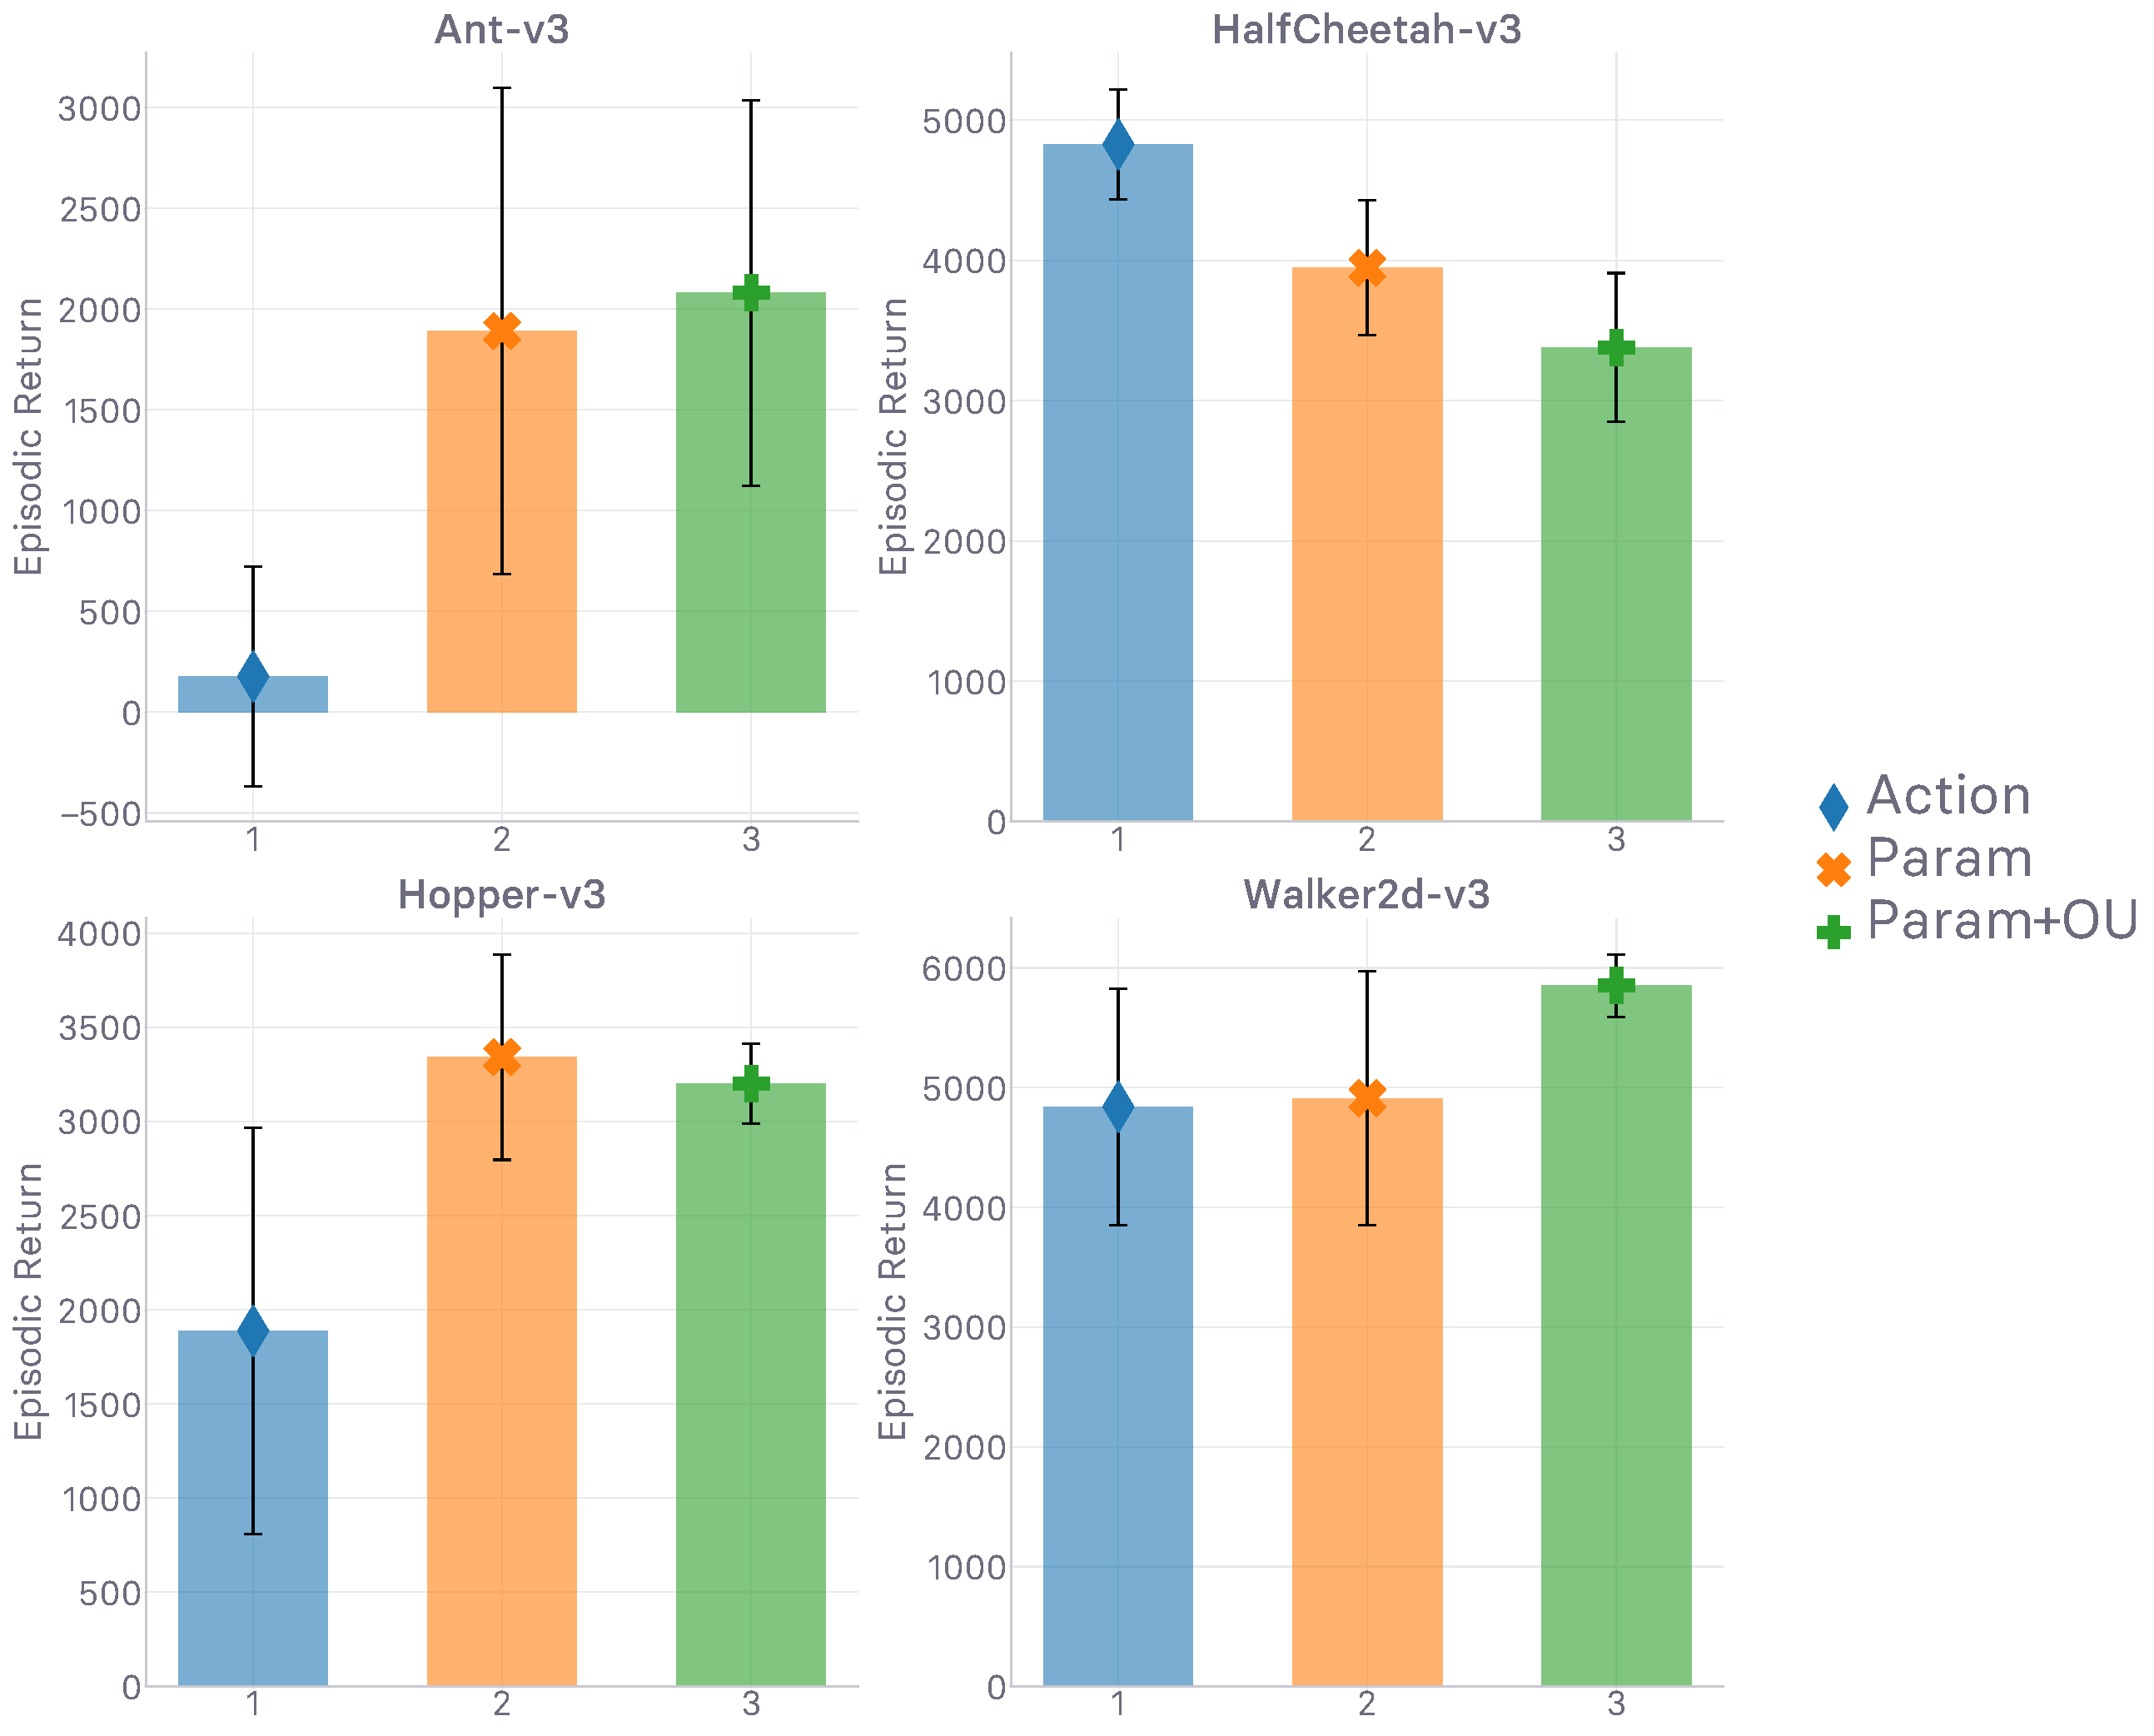
\includegraphics{Plots/fig21_explo_ablation_4envs/plots_eval_env_ret_barplot.pdf}}
    \caption{Final return values at timeout \textit{(higher is better)}}
  \end{subfigure}
  \caption{
  Evaluation of the considered method under several exploration strategies.
  \textit{``Action''} corresponds to defining $\pi_\theta$
  by directly applying additive Gaussian noise to the \emph{action} returned by $\mu_\theta$.
  As such,
  $\pi_\theta(\cdot, s_t) = \mu_\theta(s_t) + \epsilon$,
  where $\epsilon \sim \mathcal{N}(0,\sigma)$,
  with $\sigma=0.2$.
  \textit{``Param''} denotes the application of additive noise in the network \emph{parameters}
  directly, and
  \textit{``Param + OU''} corresponds to the additional application of temporally correlated
  noise, generated sequentially by a Ornstein-Uhlenbeck process, on the action
  (\textit{cf.} \textsc{Section}~\ref{bridge}
  for a description of these two last approaches,
  and \textsc{Table}~\ref{hptable} for the associated hyper-parameters).
  Despite the absence of a clear winner,
  we use the combination of parameter noise and temporally correlated action noise
  in every experiment reported in this work, as it seems to yield the best results.
  Runtime is 12 hours.}
\end{figure}
